%%%%%%%%%%%%%%%%%%%%%%%%%%%%%%%%%%%%%%%%%
%  My documentation report
%  Objetive: Explain what I did and how, so someone can continue with the investigation
%
% Important note:
% Chapter heading images should have a 2:1 width:height ratio,
% e.g. 920px width and 460px height.
%
%%%%%%%%%%%%%%%%%%%%%%%%%%%%%%%%%%%%%%%%%

%----------------------------------------------------------------------------------------
%	PACKAGES AND OTHER DOCUMENT CONFIGURATIONS
%----------------------------------------------------------------------------------------

\documentclass[12pt]{book} % Default font size

%\usepackage[top=3cm,bottom=3cm,left=3.2cm,right=3.2cm,headsep=10pt,letterpaper]{geometry} % Page margins original
\usepackage[top=3cm,bottom=3cm,left=3.2cm,right=3.2cm,headsep=10pt,a4paper]{geometry}

\usepackage{xcolor} % Required for specifying colors by name
\definecolor{ocre}{RGB}{52,177,201} % Define the orange color used for highlighting throughout the book

% Font Settings
\usepackage{avant} % Use the Avantgarde font for headings
%\usepackage{times} % Use the Times font for headings
%\usepackage{mathptmx} % Use the Adobe Times Roman as the default text font together with math symbols from the Sym­bol, Chancery and Com­puter Modern fonts

\usepackage{microtype} % Slightly tweak font spacing for aesthetics
\usepackage[utf8]{inputenc} % Required for including letters with accents
\usepackage[T1]{fontenc} % Use 8-bit encoding that has 256 glyphs
\usepackage{lmodern}
\usepackage{transparent}

% Bibliography
\usepackage[style=numeric-comp,sorting=none,natbib=true]{biblatex}
\addbibresource{thesis_bibliography.bib} % BibTeX bibliography file
\defbibheading{bibempty}{}

%\bibliographystyle{mnras}
%\usepackage{graphicx}    % Include figure files
%\usepackage{dcolumn}     % Align table columns on decimal point
%\usepackage{bm}          % bold math
%\usepackage{amssymb,amsmath}  
%\usepackage{color}
\usepackage{hyperref}
%\usepackage{lineno}
\usepackage{cleveref}
%\usepackage{natbib}
%\usepackage{amsbsy}
\usepackage{overpic}
\usepackage[titletoc]{appendix}
\usepackage{tikz}
\usepackage{rotating}

%----------------------------------------------------------------------------------------
%	VARIOUS REQUIRED PACKAGES
%----------------------------------------------------------------------------------------

\usepackage{titlesec} % Allows customization of titles

\usepackage{graphicx} % Required for including pictures
\graphicspath{{Pictures/}} % Specifies the directory where pictures are stored

\usepackage{lipsum} % Inserts dummy text

\usepackage{tikz} % Required for drawing custom shapes

\usepackage[english]{babel} % English language/hyphenation

\usepackage{enumitem} % Customize lists
\setlist{nolistsep} % Reduce spacing between bullet points and numbered lists

\usepackage{booktabs} % Required for nicer horizontal rules in tables

\usepackage{eso-pic} % Required for specifying an image background in the title page

%----------------------------------------------------------------------------------------
%	MAIN TABLE OF CONTENTS
%----------------------------------------------------------------------------------------

\usepackage{titletoc} % Required for manipulating the table of contents

\contentsmargin{0cm} % Removes the default margin
% Chapter text styling
\titlecontents{chapter}[1.25cm] % Indentation
{\addvspace{15pt}\large\sffamily\bfseries} % Spacing and font options for chapters
{\color{ocre!60}\contentslabel[\Large\thecontentslabel]{1.25cm}\color{ocre}} % Chapter number
{}  
{\color{ocre!60}\normalsize\sffamily\bfseries\;\titlerule*[.5pc]{.}\;\thecontentspage} % Page number
% Section text styling
\titlecontents{section}[1.25cm] % Indentation
{\addvspace{5pt}\sffamily\bfseries} % Spacing and font options for sections
{\contentslabel[\thecontentslabel]{1.25cm}} % Section number
{}
{\sffamily\hfill\color{black}\thecontentspage} % Page number
[]
% Subsection text styling
\titlecontents{subsection}[1.25cm] % Indentation
{\addvspace{1pt}\sffamily\small} % Spacing and font options for subsections
{\contentslabel[\thecontentslabel]{1.25cm}} % Subsection number
{}
{\sffamily\;\titlerule*[.5pc]{.}\;\thecontentspage} % Page number
[] 

%----------------------------------------------------------------------------------------
%	MINI TABLE OF CONTENTS IN CHAPTER HEADS
%----------------------------------------------------------------------------------------

% Section text styling
\titlecontents{lsection}[0em] % Indendating
{\footnotesize\sffamily} % Font settings
{}
{}
{}

% Subsection text styling
\titlecontents{lsubsection}[.5em] % Indentation
{\normalfont\footnotesize\sffamily} % Font settings
{}
{}
{}
 
%----------------------------------------------------------------------------------------
%	PAGE HEADERS
%----------------------------------------------------------------------------------------

\usepackage{fancyhdr} % Required for header and footer configuration

\pagestyle{fancy}
\renewcommand{\chaptermark}[1]{\markboth{\sffamily\normalsize\bfseries\chaptername\ \thechapter.\ #1}{}} % Chapter text font settings
\renewcommand{\sectionmark}[1]{\markright{\sffamily\normalsize\thesection\hspace{5pt}#1}{}} % Section text font settings
\fancyhf{} \fancyhead[LE,RO]{\sffamily\normalsize\thepage} % Font setting for the page number in the header
\fancyhead[LO]{\rightmark} % Print the nearest section name on the left side of odd pages
\fancyhead[RE]{\leftmark} % Print the current chapter name on the right side of even pages
\renewcommand{\headrulewidth}{0.5pt} % Width of the rule under the header
\addtolength{\headheight}{2.5pt} % Increase the spacing around the header slightly
\renewcommand{\footrulewidth}{0pt} % Removes the rule in the footer
\fancypagestyle{plain}{\fancyhead{}\renewcommand{\headrulewidth}{0pt}} % Style for when a plain pagestyle is specified

% Removes the header from odd empty pages at the end of chapters
\makeatletter
\renewcommand{\cleardoublepage}{
\clearpage\ifodd\c@page\else
\hbox{}
\vspace*{\fill}
\thispagestyle{empty}
\newpage
\fi}

%----------------------------------------------------------------------------------------
%	THEOREM STYLES
%----------------------------------------------------------------------------------------

\usepackage{amsmath,amsfonts,amssymb,amsthm} % For math equations, theorems, symbols, etc

\newcommand{\intoo}[2]{\mathopen{]}#1\,;#2\mathclose{[}}
\newcommand{\ud}{\mathop{\mathrm{{}d}}\mathopen{}}
\newcommand{\intff}[2]{\mathopen{[}#1\,;#2\mathclose{]}}
\newtheorem{notation}{Notation}[chapter]

%%%%%%%%%%%%%%%%%%%%%%%%%%%%%%%%%%%%%%%%%%%%%%%%%%%%%%%%%%%%%%%%%%%%%%%%%%%
%%%%%%%%%%%%%%%%%%%% dedicated to boxed/framed environements %%%%%%%%%%%%%%
%%%%%%%%%%%%%%%%%%%%%%%%%%%%%%%%%%%%%%%%%%%%%%%%%%%%%%%%%%%%%%%%%%%%%%%%%%%
\newtheoremstyle{ocrenumbox}% % Theorem style name
{0pt}% Space above
{0pt}% Space below
{\normalfont}% % Body font
{}% Indent amount
{\small\bf\sffamily\color{ocre}}% % Theorem head font
{\;}% Punctuation after theorem head
{0.25em}% Space after theorem head
{\small\sffamily\color{ocre}\thmname{#1}\nobreakspace\thmnumber{\@ifnotempty{#1}{}\@upn{#2}}% Theorem text (e.g. Theorem 2.1)
\thmnote{\nobreakspace\the\thm@notefont\sffamily\bfseries\color{black}---\nobreakspace#3.}} % Optional theorem note
\renewcommand{\qedsymbol}{$\blacksquare$}% Optional qed square

\newtheoremstyle{blacknumex}% Theorem style name
{5pt}% Space above
{5pt}% Space below
{\normalfont}% Body font
{} % Indent amount
{\small\bf\sffamily}% Theorem head font
{\;}% Punctuation after theorem head
{0.25em}% Space after theorem head
{\small\sffamily{\tiny\ensuremath{\blacksquare}}\nobreakspace\thmname{#1}\nobreakspace\thmnumber{\@ifnotempty{#1}{}\@upn{#2}}% Theorem text (e.g. Theorem 2.1)
\thmnote{\nobreakspace\the\thm@notefont\sffamily\bfseries---\nobreakspace#3.}}% Optional theorem note

\newtheoremstyle{blacknumbox} % Theorem style name
{0pt}% Space above
{0pt}% Space below
{\normalfont}% Body font
{}% Indent amount
{\small\bf\sffamily}% Theorem head font
{\;}% Punctuation after theorem head
{0.25em}% Space after theorem head
{\small\sffamily\thmname{#1}\nobreakspace\thmnumber{\@ifnotempty{#1}{}\@upn{#2}}% Theorem text (e.g. Theorem 2.1)
\thmnote{\nobreakspace\the\thm@notefont\sffamily\bfseries---\nobreakspace#3.}}% Optional theorem note

%%%%%%%%%%%%%%%%%%%%%%%%%%%%%%%%%%%%%%%%%%%%%%%%%%%%%%%%%%%%%%%%%%%%%%%%%%%
%%%%%%%%%%%%% dedicated to non-boxed/non-framed environements %%%%%%%%%%%%%
%%%%%%%%%%%%%%%%%%%%%%%%%%%%%%%%%%%%%%%%%%%%%%%%%%%%%%%%%%%%%%%%%%%%%%%%%%%
\newtheoremstyle{ocrenum}% % Theorem style name
{5pt}% Space above
{5pt}% Space below
{\normalfont}% % Body font
{}% Indent amount
{\small\bf\sffamily\color{ocre}}% % Theorem head font
{\;}% Punctuation after theorem head
{0.25em}% Space after theorem head
{\small\sffamily\color{ocre}\thmname{#1}\nobreakspace\thmnumber{\@ifnotempty{#1}{}\@upn{#2}}% Theorem text (e.g. Theorem 2.1)
\thmnote{\nobreakspace\the\thm@notefont\sffamily\bfseries\color{black}---\nobreakspace#3.}} % Optional theorem note
\renewcommand{\qedsymbol}{$\blacksquare$}% Optional qed square
\makeatother

% Defines the theorem text style for each type of theorem to one of the three styles above
\newcounter{dummy} 
\numberwithin{dummy}{section}
\theoremstyle{ocrenumbox}
\newtheorem{theoremeT}[dummy]{Theorem}
\newtheorem{problem}{Problem}[chapter]
\newtheorem{exerciseT}{Exercise}[chapter]
\theoremstyle{blacknumex}
\newtheorem{exampleT}{Example}[chapter]
\theoremstyle{blacknumbox}
\newtheorem{vocabulary}{Vocabulary}[chapter]
\newtheorem{definitionT}{Definition}[section]
\newtheorem{corollaryT}[dummy]{Corollary}
\theoremstyle{ocrenum}
\newtheorem{proposition}[dummy]{Proposition}

%----------------------------------------------------------------------------------------
%	DEFINITION OF COLORED BOXES
%----------------------------------------------------------------------------------------

\RequirePackage[framemethod=default]{mdframed} % Required for creating the theorem, definition, exercise and corollary boxes

% Theorem box
\newmdenv[skipabove=7pt,
skipbelow=7pt,
backgroundcolor=black!5,
linecolor=ocre,
innerleftmargin=5pt,
innerrightmargin=5pt,
innertopmargin=5pt,
leftmargin=0cm,
rightmargin=0cm,
innerbottommargin=5pt]{tBox}

% Exercise box	  
\newmdenv[skipabove=7pt,
skipbelow=7pt,
rightline=false,
leftline=true,
topline=false,
bottomline=false,
backgroundcolor=ocre!10,
linecolor=ocre,
innerleftmargin=5pt,
innerrightmargin=5pt,
innertopmargin=5pt,
innerbottommargin=5pt,
leftmargin=0cm,
rightmargin=0cm,
linewidth=4pt]{eBox}	

% Definition box
\newmdenv[skipabove=7pt,
skipbelow=7pt,
rightline=false,
leftline=true,
topline=false,
bottomline=false,
linecolor=ocre,
innerleftmargin=5pt,
innerrightmargin=5pt,
innertopmargin=0pt,
leftmargin=0cm,
rightmargin=0cm,
linewidth=4pt,
innerbottommargin=0pt]{dBox}	

% Corollary box
\newmdenv[skipabove=7pt,
skipbelow=7pt,
rightline=false,
leftline=true,
topline=false,
bottomline=false,
linecolor=gray,
backgroundcolor=black!5,
innerleftmargin=5pt,
innerrightmargin=5pt,
innertopmargin=5pt,
leftmargin=0cm,
rightmargin=0cm,
linewidth=4pt,
innerbottommargin=5pt]{cBox}

% Creates an environment for each type of theorem and assigns it a theorem text style from the "Theorem Styles" section above and a colored box from above
\newenvironment{theorem}{\begin{tBox}\begin{theoremeT}}{\end{theoremeT}\end{tBox}}
\newenvironment{exercise}{\begin{eBox}\begin{exerciseT}}{\hfill{\color{ocre}\tiny\ensuremath{\blacksquare}}\end{exerciseT}\end{eBox}}				  
\newenvironment{definition}{\begin{dBox}\begin{definitionT}}{\end{definitionT}\end{dBox}}	
\newenvironment{example}{\begin{exampleT}}{\hfill{\tiny\ensuremath{\blacksquare}}\end{exampleT}}		
\newenvironment{corollary}{\begin{cBox}\begin{corollaryT}}{\end{corollaryT}\end{cBox}}	

%----------------------------------------------------------------------------------------
%	REMARK ENVIRONMENT
%----------------------------------------------------------------------------------------

\newenvironment{remark}{\par\vspace{10pt}\small % Vertical white space above the remark and smaller font size
\begin{list}{}{
\leftmargin=35pt % Indentation on the left
\rightmargin=25pt}\item\ignorespaces % Indentation on the right
\makebox[-2.5pt]{\begin{tikzpicture}[overlay]
\node[draw=ocre!60,line width=1pt,circle,fill=ocre!25,font=\sffamily\bfseries,inner sep=2pt,outer sep=0pt] at (-15pt,0pt){\textcolor{ocre}{R}};\end{tikzpicture}} % Orange R in a circle
\advance\baselineskip -1pt}{\end{list}\vskip5pt} % Tighter line spacing and white space after remark

%----------------------------------------------------------------------------------------
%	SECTION NUMBERING IN THE MARGIN
%----------------------------------------------------------------------------------------

\makeatletter
\renewcommand{\@seccntformat}[1]{\llap{\textcolor{ocre}{\csname the#1\endcsname}\hspace{1em}}}                    
\renewcommand{\section}{\@startsection{section}{1}{\z@}
{-4ex \@plus -1ex \@minus -.4ex}
{1ex \@plus.2ex }
{\normalfont\large\sffamily\bfseries}}
\renewcommand{\subsection}{\@startsection {subsection}{2}{\z@}
{-3ex \@plus -0.1ex \@minus -.4ex}
{0.5ex \@plus.2ex }
{\normalfont\sffamily\bfseries}}
\renewcommand{\subsubsection}{\@startsection {subsubsection}{3}{\z@}
{-2ex \@plus -0.1ex \@minus -.2ex}
{.2ex \@plus.2ex }
{\normalfont\small\sffamily\bfseries}}                        
\renewcommand\paragraph{\@startsection{paragraph}{4}{\z@}
{-2ex \@plus-.2ex \@minus .2ex}
{.1ex}
{\normalfont\small\sffamily\bfseries}}

%----------------------------------------------------------------------------------------
%	HYPERLINKS IN THE DOCUMENTS
%----------------------------------------------------------------------------------------

% For an unclear reason, the package should be loaded now and not later
\usepackage{hyperref}
\hypersetup{hidelinks,backref=true,pagebackref=true,hyperindex=true,colorlinks=false,breaklinks=true,urlcolor= ocre,bookmarks=true,bookmarksopen=false,pdftitle={Title},pdfauthor={Author}}

%----------------------------------------------------------------------------------------
%	CHAPTER HEADINGS
%----------------------------------------------------------------------------------------

% The set-up below should be (sadly) manually adapted to the overall margin page septup controlled by the geometry package loaded in the main.tex document. It is possible to implement below the dimensions used in the goemetry package (top,bottom,left,right)... TO BE DONE

\newcommand{\thechapterimage}{}
\newcommand{\chapterimage}[1]{\renewcommand{\thechapterimage}{#1}}

% Numbered chapters with mini tableofcontents
\def\thechapter{\arabic{chapter}}
\def\@makechapterhead#1{
\thispagestyle{empty}
{\centering \normalfont\sffamily
\ifnum \c@secnumdepth >\m@ne
\if@mainmatter
\startcontents
\begin{tikzpicture}[remember picture,overlay]
\node at (current page.north west)
{\begin{tikzpicture}[remember picture,overlay]
\node[anchor=north west,inner sep=0pt] at (0,0) {\includegraphics[width=\paperwidth]{\thechapterimage}};
%%%%%%%%%%%%%%%%%%%%%%%%%%%%%%%%%%%%%%%%%%%%%%%%%%%%%%%%%%%%%%%%%%%%%%%%%%%%%%%%%%%%%
% Commenting the 3 lines below removes the small contents box in the chapter heading
%\fill[color=ocre!10!white,opacity=.6] (1cm,0) rectangle (8cm,-7cm);
%\node[anchor=north west] at (1.1cm,.35cm) {\parbox[t][8cm][t]{6.5cm}{\huge\bfseries\flushleft \printcontents{l}{1}{\setcounter{tocdepth}{2}}}};
\draw[anchor=west] (5cm,-9cm) node [rounded corners=20pt,fill=ocre!10!white,text opacity=1,draw=ocre,draw opacity=1,line width=1.5pt,fill opacity=.6,inner sep=12pt]{\huge\sffamily\bfseries\textcolor{black}{\thechapter. #1\strut\makebox[22cm]{}}};
%%%%%%%%%%%%%%%%%%%%%%%%%%%%%%%%%%%%%%%%%%%%%%%%%%%%%%%%%%%%%%%%%%%%%%%%%%%%%%%%%%%%%
\end{tikzpicture}};
\end{tikzpicture}}
\par\vspace*{230\p@}
\fi
\fi}

% Unnumbered chapters without mini tableofcontents (could be added though) 
\def\@makeschapterhead#1{
\thispagestyle{empty}
{\centering \normalfont\sffamily
\ifnum \c@secnumdepth >\m@ne
\if@mainmatter
\begin{tikzpicture}[remember picture,overlay]
\node at (current page.north west)
{\begin{tikzpicture}[remember picture,overlay]
\node[anchor=north west,inner sep=0pt] at (0,0) {\includegraphics[width=\paperwidth]{\thechapterimage}};
\draw[anchor=west] (5cm,-9cm) node [rounded corners=20pt,fill=ocre!10!white,fill opacity=.6,inner sep=12pt,text opacity=1,draw=ocre,draw opacity=1,line width=1.5pt]{\huge\sffamily\bfseries\textcolor{black}{#1\strut\makebox[22cm]{}}};
\end{tikzpicture}};
\end{tikzpicture}}
\par\vspace*{230\p@}
\fi
\fi
}
\makeatother % Insert the commands.tex file which contains the majority of the structure behind the template

%----------------------------------------------------------------------------------------
%	JOURNAL COMMANDS
%----------------------------------------------------------------------------------------

\newcommand\aap{A\&A}                % Astronomy and Astrophysics
\let\astap=\aap                          % alternative shortcut
\newcommand\aapr{A\&ARv}             % Astronomy and Astrophysics Review (the)
\newcommand\aaps{A\&AS}              % Astronomy and Astrophysics Supplement Series
\newcommand\actaa{Acta Astron.}      % Acta Astronomica
\newcommand\afz{Afz}                 % Astrofizika
\newcommand\aj{AJ}                   % Astronomical Journal (the)
\newcommand\ao{Appl. Opt.}           % Applied Optics
\let\applopt=\ao                         % alternative shortcut
\newcommand\aplett{Astrophys.~Lett.} % Astrophysics Letters
\newcommand\apj{ApJ}                 % Astrophysical Journal
\newcommand\apjl{ApJ}                % Astrophysical Journal, Letters
\let\apjlett=\apjl                       % alternative shortcut
\newcommand\apjs{ApJS}               % Astrophysical Journal, Supplement
\let\apjsupp=\apjs                       % alternative shortcut
% The following journal does not appear to exist! Disabled.
%\newcommand\apspr{Astrophys.~Space~Phys.~Res.} % Astrophysics Space Physics Research
\newcommand\apss{Ap\&SS}             % Astrophysics and Space Science
\newcommand\araa{ARA\&A}             % Annual Review of Astronomy and Astrophysics
\newcommand\arep{Astron. Rep.}       % Astronomy Reports
\newcommand\aspc{ASP Conf. Ser.}     % ASP Conference Series
\newcommand\azh{Azh}                 % Astronomicheskii Zhurnal
\newcommand\baas{BAAS}               % Bulletin of the American Astronomical Society
\newcommand\bac{Bull. Astron. Inst. Czechoslovakia} % Bulletin of the Astronomical Institutes of Czechoslovakia 
\newcommand\bain{Bull. Astron. Inst. Netherlands} % Bulletin Astronomical Institute of the Netherlands
\newcommand\caa{Chinese Astron. Astrophys.} % Chinese Astronomy and Astrophysics
\newcommand\cjaa{Chinese J.~Astron. Astrophys.} % Chinese Journal of Astronomy and Astrophysics
\newcommand\fcp{Fundamentals Cosmic Phys.}  % Fundamentals of Cosmic Physics
\newcommand\gca{Geochimica Cosmochimica Acta}   % Geochimica Cosmochimica Acta
\newcommand\grl{Geophys. Res. Lett.} % Geophysics Research Letters
\newcommand\iaucirc{IAU~Circ.}       % IAU Cirulars
\newcommand\icarus{Icarus}           % Icarus
\newcommand\japa{J.~Astrophys. Astron.} % Journal of Astrophysics and Astronomy
\newcommand\jcap{J.~Cosmology Astropart. Phys.} % Journal of Cosmology and Astroparticle Physics
\newcommand\jcp{J.~Chem.~Phys.}      % Journal of Chemical Physics
\newcommand\jgr{J.~Geophys.~Res.}    % Journal of Geophysics Research
\newcommand\jqsrt{J.~Quant. Spectrosc. Radiative Transfer} % Journal of Quantitiative Spectroscopy and Radiative Transfer
\newcommand\jrasc{J.~R.~Astron. Soc. Canada} % Journal of the RAS of Canada
\newcommand\memras{Mem.~RAS}         % Memoirs of the RAS
\newcommand\memsai{Mem. Soc. Astron. Italiana} % Memoire della Societa Astronomica Italiana
\newcommand\mnassa{MNASSA}           % Monthly Notes of the Astronomical Society of Southern Africa
\newcommand\mnras{MNRAS}             % Monthly Notices of the Royal Astronomical Society
\newcommand\na{New~Astron.}          % New Astronomy
\newcommand\nar{New~Astron.~Rev.}    % New Astronomy Review
\newcommand\nat{Nature}              % Nature
\newcommand\nphysa{Nuclear Phys.~A}  % Nuclear Physics A
\newcommand\pra{Phys. Rev.~A}        % Physical Review A: General Physics
\newcommand\prb{Phys. Rev.~B}        % Physical Review B: Solid State
\newcommand\prc{Phys. Rev.~C}        % Physical Review C
\newcommand\prd{Phys. Rev.~D}        % Physical Review D
\newcommand\pre{Phys. Rev.~E}        % Physical Review E
\newcommand\prl{Phys. Rev.~Lett.}    % Physical Review Letters
\newcommand\pasa{Publ. Astron. Soc. Australia}  % Publications of the Astronomical Society of Australia
\newcommand\pasp{PASP}               % Publications of the Astronomical Society of the Pacific
\newcommand\pasj{PASJ}               % Publications of the Astronomical Society of Japan
\newcommand\physrep{Phys.~Rep.}      % Physics Reports
\newcommand\physscr{Phys.~Scr.}      % Physica Scripta
\newcommand\planss{Planet. Space~Sci.} % Planetary Space Science
\newcommand\procspie{Proc.~SPIE}     % Proceedings of the Society of Photo-Optical Instrumentation Engineers
\newcommand\rmxaa{Rev. Mex. Astron. Astrofis.} % Revista Mexicana de Astronomia y Astrofisica
\newcommand\qjras{QJRAS}             % Quarterly Journal of the RAS
\newcommand\sci{Science}             % Science
\newcommand\skytel{Sky \& Telesc.}   % Sky and Telescope
\newcommand\solphys{Sol.~Phys.}      % Solar Physics
\newcommand\sovast{Soviet~Ast.}      % Soviet Astronomy (aka Astronomy Reports)
\newcommand\ssr{Space Sci. Rev.}     % Space Science Reviews
\newcommand\zap{Z.~Astrophys.}       % Zeitschrift fuer Astrophysik


\begin{document}

%----------------------------------------------------------------------------------------
%	TITLE PAGE
%----------------------------------------------------------------------------------------

\begingroup
\thispagestyle{empty}
\pagenumbering{roman}
\setcounter{page}{1}
%\AddToShipoutPicture*{\put(0,0){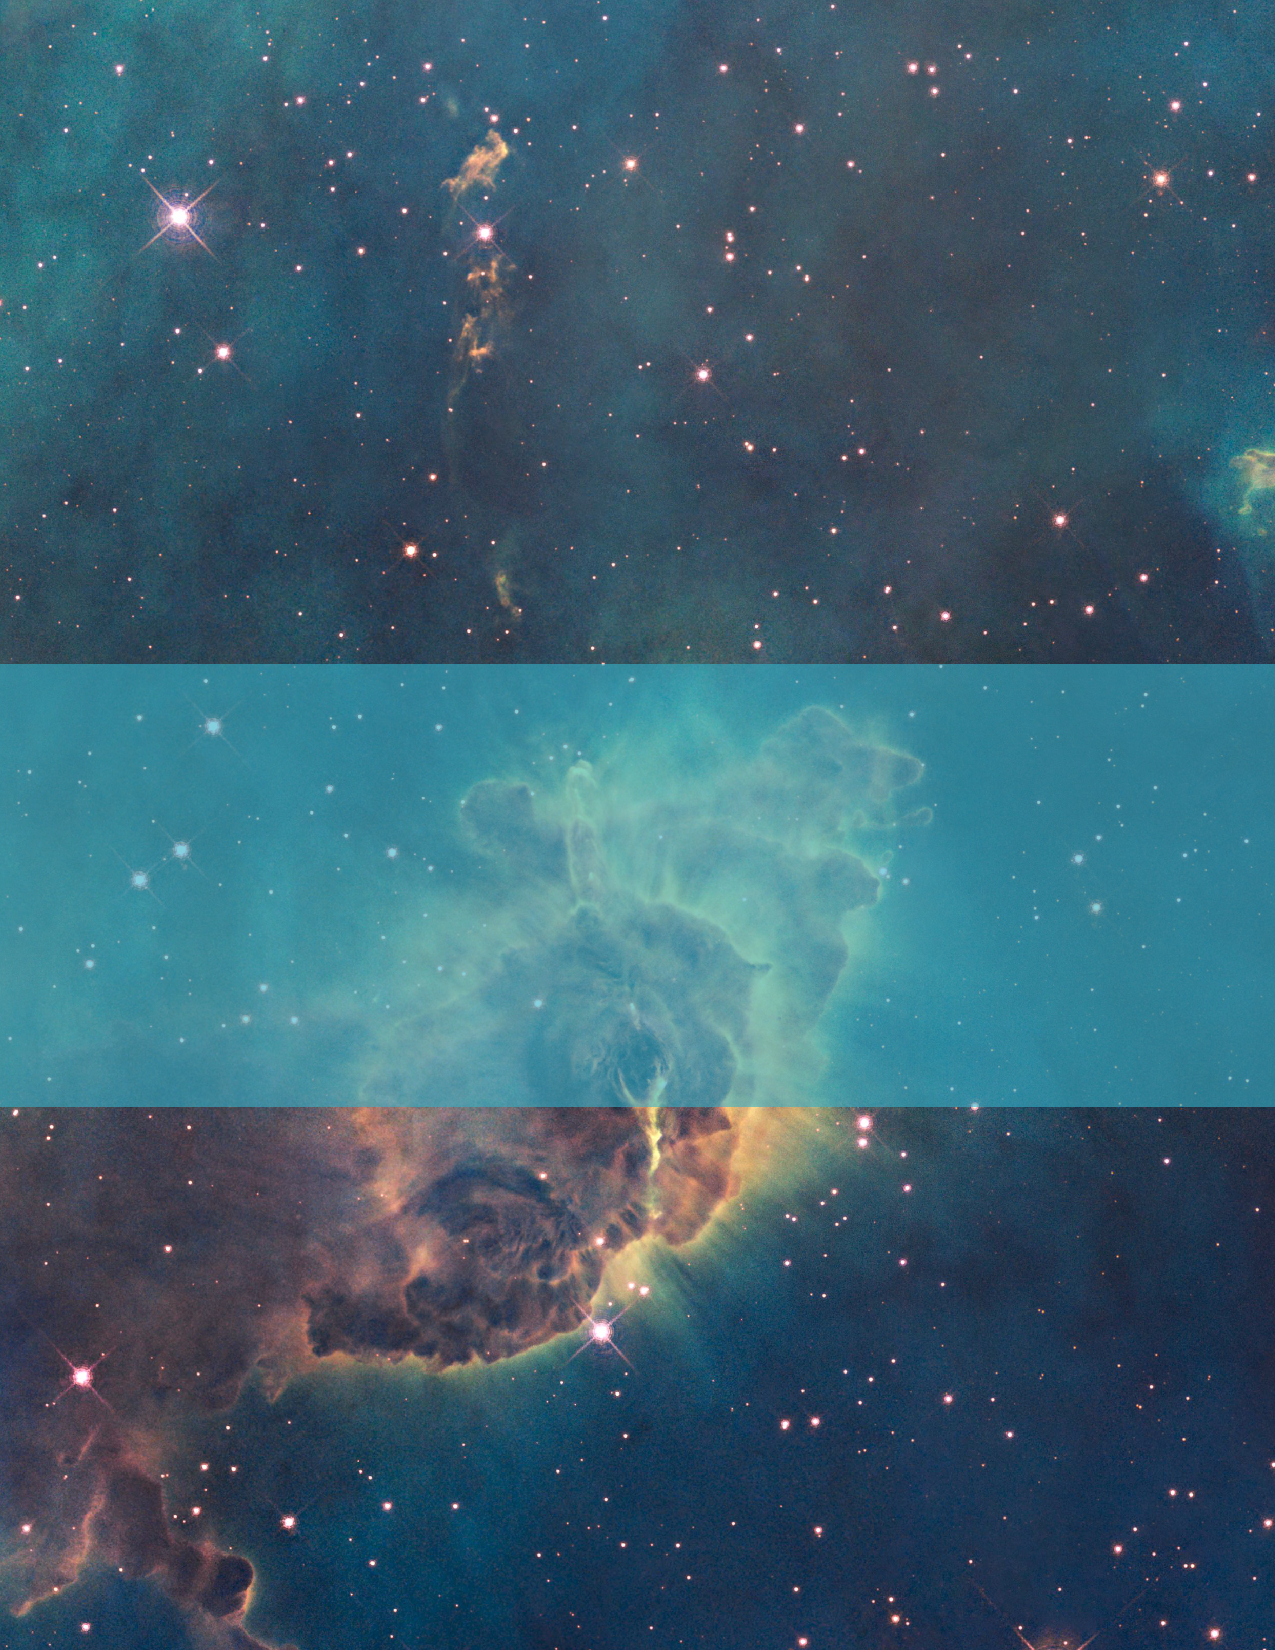
\includegraphics[scale=1.25]{esahubble}}} % Image background
%\AddToShipoutPicture*{\put(0,0){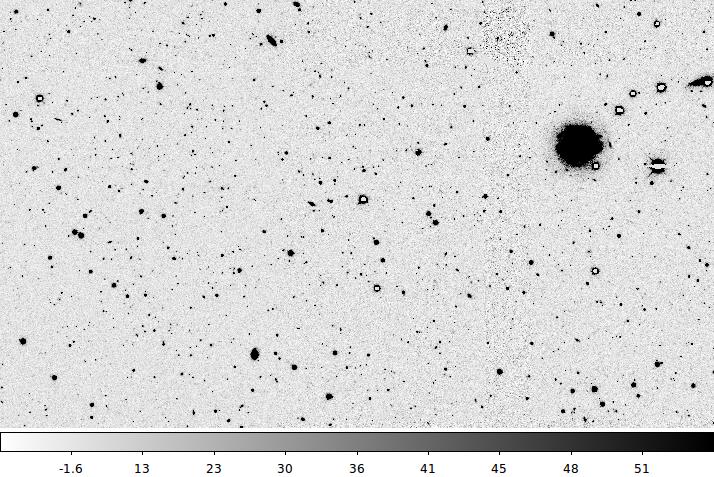
\includegraphics[height=23cm,angle=90,trim=4cm 2cm 0 0,clip]{ds9.png}}} % Image background
\AddToShipoutPicture*{\put(0,0){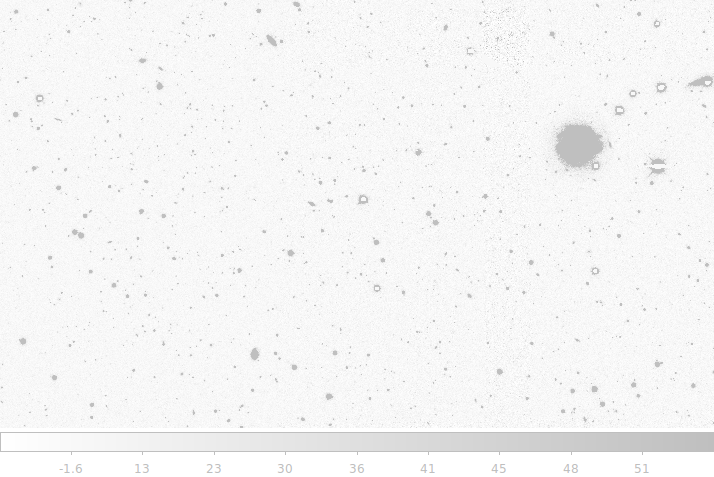
\includegraphics[height=23cm,angle=90,trim=4cm 2cm 0 0,clip]{./Pictures/ds9_transparent.png}}\put(100,50){
\includegraphics[width=\textwidth,angle=0,clip]{MDM_Banner.jpg}}} % Image background

\centering
\vspace*{5cm}
\par\normalfont\fontsize{27}{27}\sffamily\selectfont
\textcolor{blue}{\textbf{Weak-lensing magnification as a probe for the dark Universe}}\par % Book title
\vspace*{1cm}
\textcolor{blue}{\textbf{\Huge Manuel Garc\'ia Fern\'andez}}\par % Author name

\title{Weak-lensing magnification as a probe for the dark Universe}
\author{Manuel Garcia-Fernandez}
\endgroup

%----------------------------------------------------------------------------------------
%	COPYRIGHT PAGE
%----------------------------------------------------------------------------------------

\newpage
~\vfill
\thispagestyle{empty}

\newpage
\thispagestyle{empty}
\begin{center}


\includegraphics[width=0.95\textwidth]{MDM_Banner.jpg}

\includegraphics[width=0.6\textwidth]{LOGO_UAM_NEG.JPG}

\vspace{1cm}
Departamento de Investigaci\'on B\'asica -- Divisi\'on de Astrof\'isica de Part\'iculas\\
Centro de Investigaciones Energ\'eticas Medioambientales y Tecnol\'ogicas\\
\vspace{0.3cm}
{\it \&}\\
\vspace{0.3cm}
Departamento de F\'isica Te\'orica -- Facultad de Ciencias\\
Universidad Aut\'onoma de Madrid\\
\vspace{2cm}
{\bf \LARGE Weak-lensing magnification as a probe for the dark Universe}\\
\vspace{1cm}
{\bf \LARGE Magnificaci\'on por lentes gravitacionales d\'ebiles como sonda del Universo oscuro}\\
\vspace{2cm}
Tesis presentada por:\\{\it Thesis submitted by:}\\
{\bf Manuel Garc\'ia Fern\'andez}\\
Para el grado de Doctor en F\'isica Te\'orica.\\{\it For the degree of Ph.D. of Theoretical Physics.}\\
\vspace{1cm}
Dirigido por:\\
{\it Supervised by:}\\
Dr. Eusebio S\'anchez \'Alvaro\\
{\it \&}\\
Dr. Ignacio Sevilla Noarbe\\
\vspace{1cm}
Madrid, Marzo-XXX del 2017

\end{center}

\newpage
~\vfill
\thispagestyle{empty}


\newpage
\noindent
According to RD-99/2011, in partial fulfillment to obtain the `Menci\'on Internacional' qualification, this Thesis is written in English.\\
According to UAM's Normative (12/15/2011), Summary and Conclusions are also written in Spanish and included before the core of the Thesis, right after the table of contents.\\

\noindent
Conforme al RD-99/2011, en requerimiento parcial para la obtenci\'on de la calificaci\'on  de `Menci\'on Internacional', esta Tesis est\'a redactada en Ingl\'es.\\
Conforme al acuerdo del Consejo de Gobierno de la UAM (15/12/2011), el Resumen y las Conclusiones tambi\'en se encuentran redactadas en Castellano y se incluyen antes del cuerpo de la Tesis justo despu\'es del \'indice.
\vspace*{2cm}
\begin{flushleft}
\rule{\textwidth}{2pt}
This Thesis is part of the following publication archives:\\
The DES Collaboration archive: DES-2017-0265\\
%Fermilab preprint/thesis server:\\
\rule{\textwidth}{2pt}\\
\vspace*{2cm}
\noindent
Part of the results obtained during the development of this Thesis has been published under peer-review journals and proceedings. Their references are listed below.\\

\noindent
Parte de los resultados obtenidos durante el desarrollo de esta Tesis han sido publicados en revistas y conferencias con un proceso de revisi\'on por pares. Sus referencias bibliogr\'aficas se encuentran abajo.\\
\vspace*{0.5cm}
{\bf M. Garcia-Fernandez}, E. Sanchez and N. Sevilla-Noarbe. {\it Magnification with wide-field photometric surveys}. Highlights on Spanish Astrophysics XII. March 2017.\\
\vspace*{0.5cm}
{\bf M. Garcia-Fernandez} et~al. {\it Weak lensing magnification in the Dark Energy Survey Science Verification data}, arXiv:1611.10326. November 2016.

~\vfill
\thispagestyle{empty}
\begin{footnotesize}
Cover image credit: M. Garcia-Fernandez \& The DES Collaboration\\
Chapter header credit: NASA
\end{footnotesize}
\end{flushleft}

\newpage
~\vfill
\thispagestyle{empty}


\newpage
\thispagestyle{empty}
\begin{flushright}
\begin{large}
\vspace*{3cm}
{\it Hacemos una vasija\\ con un pedazo de arcilla\\ y es el espacio vac\'io\\ en el interior de la vasija\\ el que la hace \'util.}\\
\vspace{1cm}
LAO TS\'E\\
\end{large}
~\vfill
\end{flushright}

%----------------------------------------------------------------------------------------
%	TABLE OF CONTENTS
%----------------------------------------------------------------------------------------

\chapterimage{head1.png} % Table of contents heading image

\pagestyle{empty} % No headers

\tableofcontents % Print the table of contents itself

%\cleardoublepage % Forces the first chapter to start on an odd page so it's on the right

\pagestyle{fancy} % Print headers again

%----------------------------------------------------------------------------------------
%	CHAPTERS
%----------------------------------------------------------------------------------------
\chapter*{Resumen y Conclusiones}
\addcontentsline{toc}{chapter}{\color{ocre}Resumen y Conclusiones}
\section*{Resumen}
\addcontentsline{toc}{section}{Resumen}
Medidas recientes de diferentes experimentos arrojan dos efectos observacionales: el Universo es plano y se expande de forma acelerada. Estes dos resultados no est\'an permitidos simult\'aneamente en la teoria gravitatoria actual --la Relatividad General-- en su formulaci\'on original. Las alternativas a la Relatividad General que tienen en cuenta la expansi\'on acelerada en universos planos son: la constante cosmol\'ogica, la presencia de campos cu\'anticos ex\'oticos y teor\'ias de gravedad modificada. Sea cual sea la respuesta se le denomina energ\'ia oscura.
\newline

El experimento que se est\'a desarrollando actualmente que est\'a espec\'ificamente dise\~nado para desvelar la naturaleza de la energ\'ia oscura es el Dark Energy Survey (DES), que usar\'a cuatro m\'etodos para discriminar qu\'e teor\'ia es la correcta: Supernovas de tipo 1a (SNIa), el n\'umero de cl\'usteres de galaxias, las oscilaciones ac\'usticas de bariones y las lentes gravitacionales d\'ebiles.
\newline

Las lentes gravitacionales d\'ebiles son producidas por la deflexi\'on las trayectorias de los fotones en la presencia de campos gravitatorios lo que se traduce en un curvado de los rayos de luz. Esto implica que la luz emitida por galaxias lejanas es desviada por la materia localizada entre dichas galaxias y el observador. Para fuentes extensas, esto se traduce en dos efectos observacionales: un aumento is\'otropo del tamaño (magnificaci\'on) y una elongaci\'on/encogimiento a lo largo de uno de los ejes ({\it shear}).
\newline

Dado que el brillo superficial se conserva, el incremento del tama\~no debido a la magnificaci\'on produce un incremento del flujo de las galaxias que se encuentran m\'as alejadas. Esto permite ver galaxias que estar\'ian por debajo del umbral de detecci\'on is el efecto de lente gravitacional no existiese. Este efecto es conocido como {\it number-count magnification} y permite medir el perfil de convergencia de la muestra seleccionada como lente, que est\'a directamente relacionado con el perfil de materia.
\newline

En esta Tesis, se desarrolla una nueva metodolog\'ia para estudiar el efecto {\it number-count magnification} y se aplica al cat\'alogo de datos {\it Science Verification} del experimento {\it Dark Energy Survey}. Esta nueva metodolog\'ia empleada usa galaxias fuente de la poblaci\'on general de galaxias seleccionadas puramente por su {\it redshift} fotom\'etrico. Esta muestra est\'a mucho m\'as poblada, lo que permite usar lentes menos densas. Adem\'as una nueva t\'ecnica para estudiar errores sistem\'aticos con la ayuda de simulaciones se ha usado, lo que permite aportar medidas fiables y no sesgadas. Finalmente en los datos {\it Year 1} de DES se ha medido el perfil de convergencia de {\it voids} y {\it troughs} usando esta nueva metodolog\'ia.
\newline

La determinaci\'on del perfil de convergencia de {\it voids} y {\it troughs} es una forma excelente de revelar la naturaleza de la energ\'ia  oscura, dado que son grandes regiones donde hay una gran infra-densidad de materia, por lo que su evoluci\'on y estructura est\'a dominada por la energ\'ia oscura. Sin embargo, las predicciones te\'oricas del perfil de convergencia de {\it voids} en modelos de gravidad modificada no est\'an toda\'ia disponibles. Dado esto, una nueva ventana para desvelar la naturaleza de la energ\'ia oscura se a abierto  aunque a\'un necesita de desarrollo.
\section*{Conclusiones}
\addcontentsline{toc}{section}{Conclusiones}
La Relatividad General ha sido la teor\'ia gravitatoria desde que Einstein la concibiese hace un siglo. Desde entonces, ha pasado satisfactoriamente las pruebas m\'as exigentes. Sin embargo, el descubrimiento de la expansi\'on acelerada del Universo --energ\'ia oscura-- junto con los \'ultimos resultados del LHC en el campo de la F\'isica de Altas Energ\'ias sugiere que algo debe estar mal o en el campo del Model Est\'andar F\'isica de Part\'iculas o que hay algo m\'as all\'a de la Relatividad General.
\newline

Medidas de la gravedad en escalas cosmol\'ogicas puede arrojar pistas sobre la naturaleza de la energ\'ia oscura. Uno de dichos escenarios, son las regiones m\'as vac\'ias del Universo: {\it voids} y {\it troughs}. Dado que dichas regiones est\'an mayormente vac\'ias de materia, su evoluci\'on y estructura est\'a dominada por la energ\'ia oscura. Esto implica que constituyes un entorno prometedor para sondar la energ\'ia oscura.
\newline

Las medidas de las propiedades de {\it voids} y {\it troughs} se pueden hacer con el efecto de lente gravitacional d\'ebil, es decir: magnificaci\'on y {\it gg-lensing}. La ventaja de usar estes dos m\'etodos es que son efectos complementarios del mismo fen\'omeno pero son sensibles a diferentes errores sistem\'aticos. Esto implica que la combinaci\'on de estes dos m\'etodos para medir {\it voids} y {\it troughs} proporciona una medida precisa y fiable para la naturaleza de la energ\'ia oscura.
\newline

Aunque los grandes cartografiados de galaxias han producido durante los \'ultimos a\~nos numerosos resultados de lentes gravitacionales, 
\chapter*{Summary}
\addcontentsline{toc}{chapter}{\color{ocre}Summary}
Latest measurements from different experiments lead to two observational effects: the Universe is flat, and its expansion is accelerated. Previos results are not allowed at the same time with the current gravitational theory --General Relativity-- on its original formulation. The alternatives to General Relativity to take into account the accelerated expansion on flat universes are: the cosmological constant, the presence of exotic quantum fields and modified gravity theories. Whatever it's the answer it is called dark energy.
\newline

The current experiment specifically designed to unravel the nature of dark energy is the Dark Energy Survey (DES), that will use four probes to discriminate which theory is right: Type Ia Supernovae (SNIa), cluster counts, barion acoustic oscillation (BAO) and weak-lensing.
\newline

Weak-lensing is produced by the gravitational bending of the trajectory of photons by gravitational fields leading to the deflection of the light rays. Thus, the light emitted by foreground distant galaxies is deflected by the matter located between them and the observe. For extended sources, in addition to the change in position, for extended sources, this leads to two observational effects: an isotropic size enlargement (magnification) and an elongation/shrink along one axis (shear).
\newline

Since the surface brightness is preserved, the isotropic size enlargement due to magnification produces an increase on the observed flux of the background galaxies. This allows to see galaxies that would be beyond the detection threshold if gravitational lensing was not present. Since this flux augmentation is dependent on the distance to the objects that produce lensing, nearby the lenses the observed density of sources is increased. This effect is known as number-count magnification and allows to probe the convergence profile of the lens sample selected, that is a proxy for the matter profile.
\newline

On this Thesis, a methodology to study number-count magnification is developed and applied to the Dark Energy Survey Science Verification data. This new methodology employs source galaxies from the general population selected purely by photometric redshift. This sample is much more numerous, allowing to use a sample with much lower number of lenses. In addition a new technique to estimate systematic errors using simulations has been used, allowing to unbiased an reliable measurements. In additions, on the DES Year 1 data, the convergence profile of voids an troughs is determined using this new methodology.
\newline

The measurement of voids and troughs convergence profile is an excellent way to test the nature of dark energy, since they are large under-dense regions of the Universe and they are environments whose evolution is dominated by dark energy. Nevertheless, theoretical work on the convergence profile of voids is still not available. Thus a new window to test dark energy has been opened with this study that still needs to keep development.
\mainmatter
\chapterimage{head2.png} % Chapter heading image
\chapter{Introduction}
Nature's change and evolution is produced by the dynamics of the bodies and systems contained within the Universe. All the interactions of Universe can be described in terms of the four Fundamental Forces: gravitation, weak, electromagnetic and strong in ascending order of relative strength. High Energy Physics was able to unify the weak, electromagnetic and strong forces in terms of a $SU(3)\times SU(2)\times U(1)$ symmetry group in what is known as the {\it Standard Model} \cite{halzen1984quarks,peskin1995introduction,weinberg1995quantum,weinberg1996quantum,2000hep.ph....1283N}. Nevertheless, attempts to unify Gravitation with the other forces has still not provided satisfactory results.
\newline

The current consensus theory of gravitation is Einstein's General Relativity, that describes gravity as a universal deformation ($h_{\mu\nu}$) of the Minkowski metric tensor ($\eta_{\mu\nu}$)
\begin{equation}
g_{\mu\nu}(x^\lambda) = \eta_{\mu\nu}+h_{\mu\nu}(x^\lambda),
\end{equation}
where $g_{\mu\nu}$ is the metric tensor of the Universe. Gravity is postulated as a massless spin-two field with self-interaction Lagrangian
\begin{equation}
\mathcal{L}[g_{\mu\nu}] = \frac{c^4}{16\pi G_N}\sqrt{-g}g^{\mu\nu}R_{\mu\nu}(g),
\end{equation}
that couples minimally and universally to all the fields of the Standard Model; where $R_{\mu\nu}$ is the Ricci tensor, $c$ the speed of light and $G_N$ Newton's constant \cite{PhysRev.138.B988,feynman1995feynman,1969ApJ...157..857F,PhysRevD.33.3613,0264-9381-4-5-024,0264-9381-4-5-025,Olive:2016xmw}.
\newline

From the total action, Einstein's equation of the gravitational field can be obtained \cite{ANDP:ANDP19163540702,1916AnP...354..769E}:
\begin{equation}
R_{\mu\nu}-\frac{1}{2}Rg_{\mu\nu} = \frac{8\pi G_N}{c^4}T_{\mu\nu},
\label{eq:einsteinbare}
\end{equation}
where $T_{\mu\nu}$ is total energy-momentum tensor, that is the source of gravity.

\section{The expanding Universe}
\begin{figure}
\begin{center}
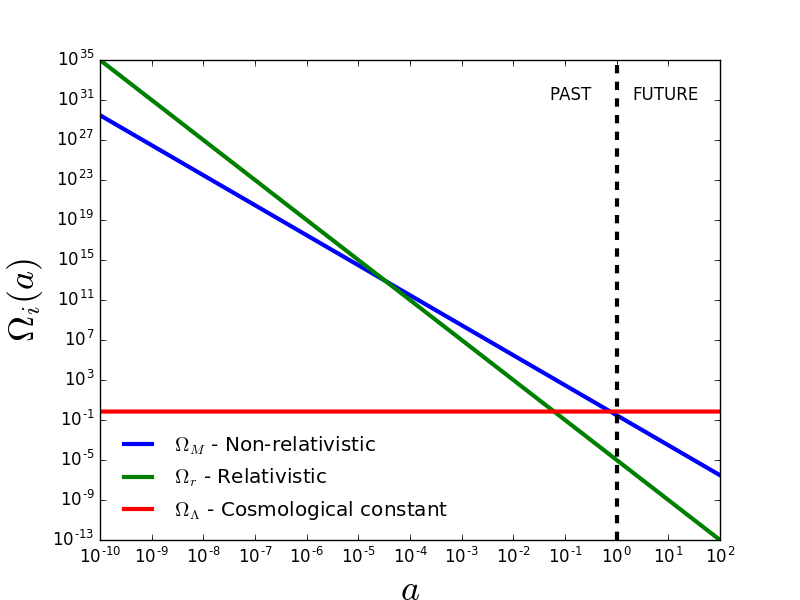
\includegraphics[width=0.75\textwidth]{./Pictures/rho_a.png}
\caption{Critical energy density for different types of matter species as function of the scale parameter of the Universe: relativistic (cold matter), non-relativistic (radiation), and cosmological constant. It can be seen that at present (black-dashed line), cosmological constant has just started to be dominant over the other species, starting the accelerated expansion era.}
\label{fig:rho_de}
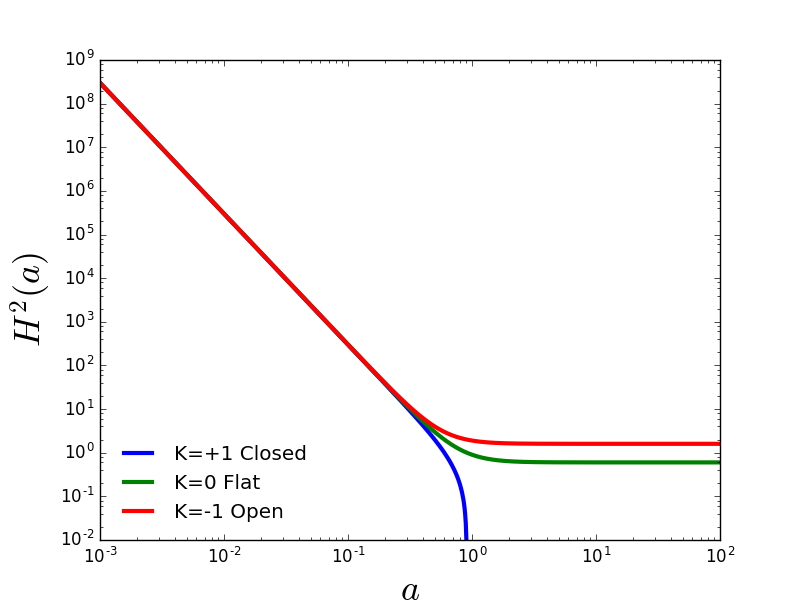
\includegraphics[width=0.75\textwidth]{./Pictures/scale_factor.png}
\caption{Expansion rate as function of the scale parameter of the Universe for different geometries (assume $\Omega_M=1$). The flat geometry expansion rate decreases until at infinity reaches zero. Open geometries show a constant expansion rate leading to an exponential growth of the scale factor. Closed geometries drops to zero very fast an eventually becomes negative leading to a re-collapse of the Universe.}
\label{fig:scale_geometry}
\end{center}
\end{figure}
One of the consequences of Einstein's equation is that the metric tensor is not static, implying that the geometry of the Universe changes. Thus, the Universe is a dynamical entity itself and its past and future evolution can be computed withing the framework of General Relativity.
\newline

Assuming that the Universe is homogeneous and isotropic \citep{2014MNRAS.440...10A,2015MNRAS.449..670A}, the only possible metric tensor is the Friedman-Lema\^itre-Robertson-Walker metric (FLRW) given by the line element \cite{1927ASSB...47...49L}
\begin{equation}
ds^2 = -dt^2+a^2(t)\left[\frac{dr^2}{1-Kr^2}+r^2(d\theta^2+\sin^2\theta d\phi^2)\right],
\end{equation}
where $a(t)$ is a function of time know as scale factor, $K=-1,0,1$ is the curvature of the universe and $r,\theta,\phi$ are spatial 3D spherical coordinates.
\newline

Solving Einstein's equation for this metric, an expression for the evolution of the scale factor with time can be obtained
\begin{equation}
H^2(t)\equiv \left[\frac{\dot a(t)}{a(t)}\right]^2 = \frac{8\pi G_N}{3c^4}\rho(t) -\frac{K}{a^2(t)},
\end{equation}
where the dot denotes time derivatives, and $\rho$ is the total density of energy. The parameter $H$ has been defined as the expansion rate and its value at present $H_0$ is known as Hubble's constant.
\newline

Expansion rate can be expressed in terms of the critical energy density
\begin{equation}
H^2(t) = H_0^2\left[\sum_i\Omega_i(t)-\Omega_K\right]
\label{eq:flrw}
\end{equation}
with
\begin{equation}
\Omega_K\equiv\frac{K}{[a(t)H_0]^2}\ \ \mbox{ and }\ \ \Omega_i(t)\equiv \frac{8\pi\rho_i(t)}{3H_0^2}.
\end{equation}
The parameter $\Omega_i$ is the critical density of the $i$-th matter/energy specie whose evolution with time can be computed using Thermodynamics. For non-relativistic matter --that is, matter with velocity $v\ll c$--, 
\begin{equation}
\Omega_M(t) = \Omega_M^0a^{-3}(t),
\end{equation}
whereas for relativistic matter species --that is, $v\sim c$-- also known as radiation,
\begin{equation}
\Omega_r(t) = \Omega_r^0 a^{-4}(t).
\end{equation}
Here $\Omega_i^0$ denotes the value on the present day of the $i$-th matter specie and by construction
\begin{equation}
\sum_i\Omega_i^0=1+\Omega_K
\label{eq:conservationenergy}
\end{equation}
\newline

Taking into account that the matter species and the curvature evolve on a different manner with time (\autoref{fig:rho_de}), its relative abundance at present fixes the expansion rate for the whole history of the Universe from birth to death. Discarding the hypothesis of empty Universe\footnote{At least, this Thesis is present at the Universe, therefore it is not empty.} and taking into account that for $a\rightarrow\infty$ all the matter species are diluted, three scenarios of expansion history can be considered depending on the curvature density of the Universe (\autoref{fig:scale_geometry}):
\begin{itemize}
\item {\bf Big Crunch:} Universe closed, with positive curvature ($K=1$). The attractive gravitational self-interaction of the Universe causes the gravitational collapse of the whole Universe into a single point.
\item {\bf Big Rip:} The Universe has negative curvature ($K=-1$), the gravitational repulsive self-interaction of the Universe causes a perpetual accelerated expansion.
\item {\bf Big Freeze:} The Universe is flat ($K=0$) and expands forever at a decelerated rate until it stops at $a\rightarrow\infty$.
\end{itemize}

Thus, the curvature of the Universe is the critical parameter to determine its thermal history. The latest combination of different cosmological probes determine it to be $\Omega_K = -0.0001^{+0.0054}_{-0.0052}$ \cite{2015arXiv150201589P}, quantity close to the floor of experimental accuracy \cite{2016PhRvD..94b3502L}, allowing to assume safely that the Universe is flat. Thus, the Universe is expected to be expanding at a decelerated rate. Although, the expansion of the Universe has been known for a century since Hubble's measurement of the recession velocity of galaxies \cite{1929PNAS...15..168H}, measurements of type-Ia supernovae (SNIa) two decades ago and  confirmed since then by several probes \cite{2008ARA&A..46..385F} show that the expansion of the Universe is accelerating (\autoref{fig:sdss_flatness} and \autoref{fig:sarkar_SNIa}).
\begin{figure}
\begin{center}
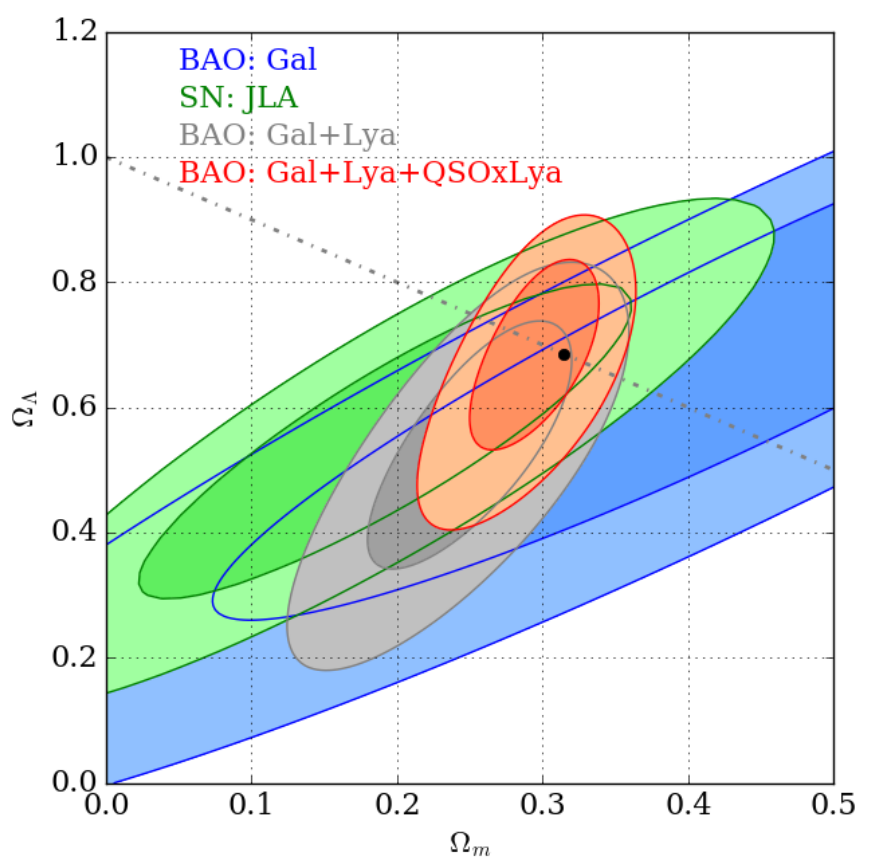
\includegraphics[width=0.7\textwidth]{./Pictures/omega_K_sdss.png}
\caption{Latest constrains on the curvature of the Universe measured by the combination of barion acoustic oscillation (BAO) and supernovas (SN) \cite{2017arXiv170200176B}. Curvature can be obtained with \autoref{eq:conservationenergy} assuming that the matter species are only dark energy and non-relativistic matter, $\Omega_\Lambda,\Omega_M$ respectively. Black-solid dot is Planck 2015 best-fit result \cite{2015arXiv150201589P}. Flat Universe is the dash-dotted line.}
\label{fig:sdss_flatness}
\vspace*{0.3cm}
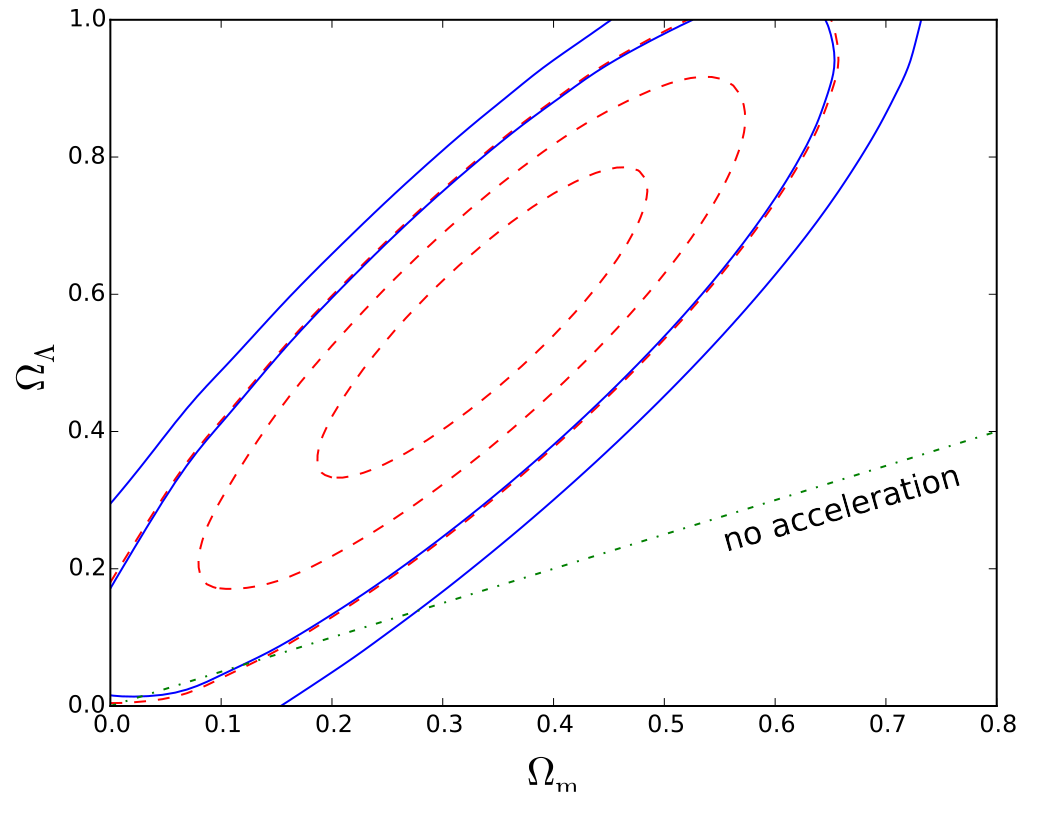
\includegraphics[width=0.7\textwidth]{./Pictures/sarkar_acceleration.png}
\caption{Reanalysis by J. T. Nielsen et~al. of the Nobel Laureate SNIa data, demonstrating that accelerated expansion is solid \cite{2016NatSR...635596N}.}
\label{fig:sarkar_SNIa}
\end{center}
\end{figure}

\section{Dark Energy Models}
Two independent experiments of different properties of the Universe show contradictory measurements: the Universe is flat and its expansion is accelerated. This implies two things, either \autoref{eq:einsteinbare} is wrong or the Universe is filled with new matter specie, that does not dilute with cosmic expansion and has negative pressure. Whatever drives this accelerated expansion is known as Dark Energy. Dark Energy models can be divided in three categories: the cosmological constant, exotic matter fields and modified gravity.
\newline

Among all the possible explanations, the cosmological constant is considered the fiducial explanation for dark energy.

\subsection{The Cosmological Constant}
The Cosmological Constant was initially proposed by Einstein himself \cite{1917SPAW.......142E} to avoid the solutions of the General Relativity where the Universe was not static and later discarded, when the expansion of the Universe was discovered by Hubble. Nevertheless, on the light of the recent events of accelerated expansion, the Cosmological Constant was soon recovered. The approach followed by this model consist on the addition of an additional covariant term to the Einstein field equations, a term proportional to the metric tensor ($\Lambda g_{\mu\nu}$), resulting \cite{2001LRR.....4....1C}:
\begin{equation}
R_{\mu\nu}-\frac{1}{2}Rg_{\mu\nu}+\Lambda g_{\mu\nu} = \frac{8\pi G_N}{c^4}T_{\mu\nu}.
\end{equation}
With this new term and assuming $\Omega_K=0$ \autoref{eq:flrw} transforms into
\begin{equation}
H^2(t) = H_0^2\left[\sum_i\Omega_i(t) +\Omega_\Lambda\right],
\end{equation}
where $\Omega_\Lambda$ is the dark energy critical density. This new term is a time-independent constant that has the same value on every location of the Universe. Thus, as the other matter species has a critical density that decreases with time, the dark energy critical density has only impact at late cosmic times.
\newline

This new term may be regarded as a new matter specie such that
\begin{equation}
\rho_\Lambda = \frac{3H_0^2}{8\pi G_N}\Omega_\Lambda.
\end{equation}
Taking into account \autoref{eq:conservationenergy}, an upper bound on the dark energy density can be established
\begin{equation}
\rho_v \leq \frac{3H_0^2}{8\pi G_N} \sim 10 ^{-47} \mbox{ GeV}^4.
\end{equation}
\newline

Since this energy density is fills the whole Universe and is an inherent property of the geometry of the Universe and hence of the Universe itself, from a physical point of view it can be identified as the energy of the vacuum \cite{RevModPhys.61.1,2003PhR...380..235P}. Quantum Field Theory (QFT) states that the quantum vacuum is not empty and static but it actually is a dynamical entity where particle and antiparticles are constantly produced and annihilated as it has been demonstrated by the Casimir effect. Energy density of the vacuum can be estimated
\begin{equation}
\rho_{QFT} = \int\limits_0^{1/L_P} dk \sqrt{k^2+m^2}\frac{4\pi k^2}{(2\pi)^4}\sim 10^{71}\mbox{ GeV}^4,
\end{equation}
where $L_P$ is Planck's length. Thus, there's a miss-match between the amount of dark energy measured and that predicted by QFT of several orders of magnitude. It can be argued that although it is known that Planck's energy scale is the upper range of validity of Standard Model physics, nothing prevents that it starts to fail at lower scales. A lower bound on this point can be established as the Quantum Cromodynamics (QCD) cutoff scale ($\sim 200$ MeV), leading to a vacuum energy density of
\begin{equation}
\rho_{QCD} = \int\limits_0^{1/L_{QCD}} dk \sqrt{k^2+m^2}\frac{4\pi k^2}{(2\pi)^4}\sim 10^{-3}\mbox{ GeV}^4,
\end{equation}
reducing the tension between theory and experiment, but still being catastrophic. Some theories claim that a cancellation of modes may arise at super-symmetry models. Nevertheless, latests LHC results excluded most of the phase-space of supersymmetric models \cite{2015arXiv150603091B}.
\newline

Several discrepancies indicate that either something is missing on the High Energy Physics side or on the Cosmology side. Nevertheless, it can be argued that no connection between the cosmological constant and quantum theory exists and define the cosmological constant as a free parameter of the theory. Despite this, a fine tune problem arises: the coincidence problem. As it has been observed by many experiments, the present day dark energy and matter density are very close, allowing the formation of structure. The redshift at which matter and dark energy densities are equal is given by
\begin{equation}
z_{eq} = \sqrt[3]{\frac{\Omega_\Lambda^0}{1-\Omega_\Lambda^0}}-1
\label{eq:equality}
\end{equation}
with $\Omega_\Lambda^0\in(0,1)$. Current measurements indicate that $\Omega_\Lambda^0\sim0.7$, demanding that $z_{eq}\sim0.3$. Those redshifts such that $z<z_{eq}$ are dominated by dark energy, inhibiting structure formation. The variation of \autoref{eq:equality} with dark energy density is not smooth and variations on this parameter lead to completely different results. An  increase of the 20\% on the dark energy density leads to a value of $z_{eq}=2.7$, preventing structure formation, whereas a decrease of the 20\% leads to $z_{eq}=-0.1$, indicating the universe is still matter dominated, preventing the detection of cosmic expansion. This fine tuning issue indicates that there must be some mechanism that couples dark energy and matter. Anthropic arguments can be made, stating that the value of the dark energy density has the value we measure since it is the only possible compatible with the detection of cosmic acceleration and structure formation.
\subsection{Exotic matter fields}
Since no satisfactory explanation has been found on the vacuum to explain dark energy, the presence on new quantum fields that, on the simplest case, interact only trough gravity, but on more complicated scenarios may also couple arbitrarily with the other matter fields can be considered.
\newline

The simplest case is known as quintessence and is defined as a scalar field that is added to the Lagrangian defined at \autoref{eq:einsteinbare} such that such that
\begin{equation}
\mathcal{L}[g_{\mu\nu}] = \sqrt{g}\left(g^{\mu\nu}R_{\mu\nu}(g)+\mathcal{L}_\phi\right)\ \ \mbox{ with }\ \ \mathcal{L}_\phi = -\frac{1}{2}g^{\mu\nu}\partial_\mu\phi\partial_\nu\phi-V(\phi),
\end{equation}
where $V(\phi)$ is the potential of the field. On an FLRW metric, this leads to a substance with density and pressure 
\begin{equation}
P_\phi = \frac{1}{2}\dot\phi^2-V(\phi)\ \ \mbox{ and }\ \ \rho_\phi=\frac{1}{2}\dot\phi^2+V(\phi).
\end{equation}
This can be parametrized as an ideal fluid with equation of state
\begin{equation}
w_{DE} = \frac{P_\phi}{\rho_\phi} = \frac{\dot\phi^2-2V(\phi)}{\dot\phi^2+2V(\phi)}.
\end{equation}
Thus, it can be deduced that dark energy critical density evolves with the scale factor of the universe as
\begin{equation}
\Omega_\Lambda(t) = \Omega_\Lambda^0 [a(t)]^{-3(1+w_\phi)}.
\end{equation}
\newline

The only possible candidate for dark energy as quintessence within the Standard Model of Particle Physics is the Higgs field, a complex scalar-field that fills the Universe and couples to gauge bosons giving them its mass. The potential of the field is given by
\begin{equation}
V(\phi) = \mu_H^2\phi^\dagger\phi+\frac{1}{4}\lambda_H(\phi^\dagger\phi)^2,
\end{equation}
with $\mu_H$ the mass term, $\lambda_H$ the self-interaction of the field and $\phi,\phi^\dagger$ the Higgs field and its hermitian conjugate respectively. Since the potential of the field is time independent, this leads to an equation of state
\begin{equation}
w_{DE} = \frac{-2V(\phi)}{2V(\phi)} = -1,
\end{equation}
recovering the cosmological constant solution. Thus, cosmological constant can be interpreted as the expected value of Higgs field at vacuum
\begin{equation}
\langle 0|\phi_0|0\rangle = \frac{|\mu_H|}{\sqrt{\lambda_H}}= \sqrt{\frac{1}{\sqrt{2}G_F}}= 246\mbox{ GeV},
\end{equation}
where $G_F$ is the Fermi constant, that can be computed from the decay of the muon. The connection between the decay of the muon and the Higgs field comes from the fact that the decay is mediated by vector bosons, whose mass is given by the Higgs field:
\begin{equation}
\mu^- \rightarrow W^- + \nu_\mu \mbox{ and }W^-\rightarrow e^-+\bar\nu_e.
\end{equation}
\newline

Other High Energy Physics scalar potentials can be built from physics beyond the Standard Model, such us supergravity \cite{1999PhLB..468...40B,1999astro.ph.12005B,2000PhRvD..61j3502B}, where a scalar potential can be found such that
\begin{equation}
V(\phi) = M^{4+n}\phi^{-n},\exp(\alpha\phi^2/m^3_P),
\end{equation}
which has a minimum with $w_{DE}\simeq -0.8$, close to the cosmological constant value. Within a supersymmetry breaking framework, a field with potential 
\begin{equation}
V(\phi) = M^{4+n}\phi^{-n}
\end{equation}
can be introduced \cite{1999PhRvD..60f3502B}. Nevertheless most of the phase space of supersymmetry and supergravity has been excluded by latest LHC results.
\newline

The existence of an ultra-light Pseudo-Nambu-Goldstone Boson may be postulated with an associated field with potential \cite{PhysRevLett.75.2077,1992PhRvD..45.2674F}
\begin{equation}
V(\phi) = M^4\cos^2(\phi/f).
\end{equation}
Light-massive Pseudo-Nambu-Goldstone Bosons can be found as exotic forms of matter such as axions and schizons, whose existence is far from being probed.
\newline

More complicated field models can be considered increasing the number of fields and letting them interact and will not be considered here since they are beyond the scope of this Thesis. A detailed description of all the models can be found at \cite{2010deto.book.....A}. Nevertheless, a general phenomenological description can be made in terms of the equation of state of dark energy,
\begin{equation}
P_{DE} = w_{DE}\rho_{DE}
\end{equation}
expanding the parameter $w_{DE}$ in a power series of the scale factor
\begin{equation}
w_{DE}(t) = w_0 +w_a[1-a(t)],
\end{equation}
where $w_0$ denotes the value of the equation of state parameter at present and $w_a$ is evolution --at first order-- with time. The cosmological constant may be considered as an specific solution of this equation of state where
\begin{equation}
w_0=-1\ \ \mbox{ and }\ \ w_a=0.
\end{equation}

\subsection{Modified Gravity}
Attempts to explain the existence of a cosmological constant from High Energy Physics side, leads to a tension between General Relativity and the Standard Model. Possible new exotic fields that may explain late-time cosmic acceleration are walking a tightrope due to latest LHC results from physics beyond the Standard Model.
\newline

The remaining approach to explain the accelerated expansion of the Universe is to consider General Relativity as an approximate gravitational theory on the same way Newtonian gravity is the low-energy limit of Einstein's gravity. Extensions to General Relativity are known as modified gravity models. This kind of models were born as alternate theories to dark matter as explanation of Vera Rubin's measurements of the rotation curve of spiral galaxies \cite{1982ApJ...253...70B,1983Sci...220.1339R,1985ApJ...289...81R,1985ApJ...297..423B}. 
\newline

The first theory is Milgrom's Modified Ordinary Newtonian Dynamics (MOND)  and its relativistic extensions \cite{1983ApJ...270..365M,1984ApJ...286....7B,1997ApJ...480..492S,1994ApJ...429..480B}, that suggest that Newton's second law is not valid on galactic scales, not requiring the existence of dark matter. Although some tests on galactic scales support MOND \cite{2011PhRvL.106l1303M,2013PhRvL.111d1105M}, this paradigm can not explain the Bullet Cluster \cite{2006ApJ...648L.109C,2006ApJ...652..937B,2007MNRAS.382...29B} (see \autoref{fig:bullet}). Recently Verlinde proposed a new theory that postulates gravity as a consequence of quantum entanglement at the microscopic level \cite{2016arXiv161102269V}. Although, this theory recovers MOND results for point masses, it has been rapidly put in tension with the measurement of the rotation curve of galaxies \cite{2017MNRAS.468L..68L}.
\begin{figure}
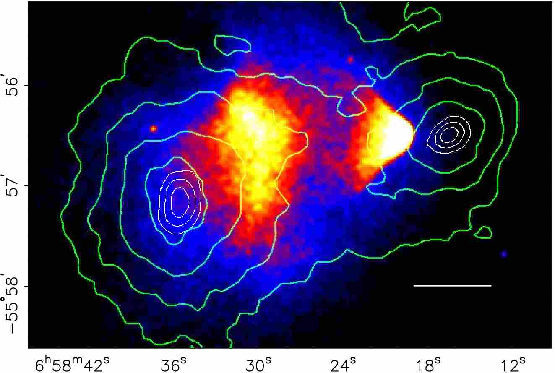
\includegraphics[width=\textwidth]{./Pictures/bullet_cluster.png}
\caption{Bullet cluster. Colors indicate the barionic mass measured with gamma-rays, whereas the solid lines indicate the mass reconstructed with gravitational lensing. This result is considered the clearest probe of the existence of dark matter and that it is decoupled from barionic matter. Image taken from \cite{2008PhRvD..78j4004D}.}
\label{fig:bullet}
\end{figure}
\newline

More elaborated theories that do not break the equivalence principle can be made. One class of those theories is known as $f(R)$ gravity \cite{2010LRR....13....3D,2010RvMP...82..451S}, and its approach is to let the Lagrangian to be a general function ($f$)
of the Ricci scalar, $R=g^{\mu\nu}R_{\mu\nu}$:
\begin{equation}
\mathcal{L}[g_{\mu\nu}] = \frac{c^4}{16\pi G_N}\sqrt{-g}f(R),
\end{equation}
that leads to the field equation
\begin{equation}
R_{\mu\nu}-\frac{1}{2}Rg_{\mu\nu}=\frac{8\pi G_N}{c^4}( T_{\mu\nu}+T_{\mu\nu}^R).
\end{equation}
This field equation is similar to \autoref{eq:einsteinbare} but has an additional term $T_{\mu\nu}^R$ that takes into account the additional curvature terms that can be modeled as a fluid on the same way as the energy-momentum tensor. The simplest case is $f(R) =R+\alpha R^n$ with $\alpha,n\in\mathbb{R}$. It has interesting cosmological solutions \cite{PhysRevD.85.083511}, nevertheless the latest studies on the large-scale-structure of the Universe, favor $\Lambda$CDM over $f(R)$ models \cite{2013PhRvD..88d4050A} although a range of $n$ can not still be fully discarded. This theory has very distinctive phenomenology such as double Einstein rings on the strong lensing regime \cite{2011PhRvD..83b4030N} that --if found-- could be the smoking gun of these kind of theories.
\newline

More complicated models of modified gravity can be considered but are not going to be treated here since they are beyond of the scope of this Thesis. For a review it can be consulted \cite{2015CQGra..32x3001B}. The usual approach to explore the modifications to General Relativity \cite{2015PhRvD..91h3504L} are to model the departures of the metric. On the Newtonian gauge, the FLRW line element of can be parametrized with the Newtonian and the lensing potential; $\Phi,\Psi$ respectively \cite{2015PhRvD..91h3504L}:
\begin{equation}
ds^2 = a^2(\tau)[-(1+2\Phi)d\tau^2+(1-2\Phi)dx_idx^j],
\end{equation}
with
\begin{equation}
2\nabla^2\Phi(a,k) = \frac{8\pi G_N}{c^2}a^2\mu(a,k)\bar \rho_M\delta_M(a,k)\ \ \mbox{ and }\ \ \gamma(a,k)=\frac{\Phi(a,k)}{\Psi(a,k)},
\end{equation}
where $\bar \rho_M$ is the average matter density, $\delta_M$ its fluctuations and $k$ is the wavenumber of the potentials. Here $\mu$ and $\gamma$ parametrize the departures from General Relativity, that is the specific case with
\begin{equation}
\mu(a,k) = 1\ \ \mbox{ and }\ \ \gamma(a,k) = 1.
\end{equation}

It is important to remark that the zoo all the departures from General Relativity plus cosmological constant --including the addition of new fields--, may be unified into a single parametrization known as Parametrized Post-Friedmann Framework \cite{2013PhRvD..87b4015B}.

\section{Current status of Dark Energy constrains}
The latest and more precise results constraining dark energy are provided by the Planck Collaboration 2015 results from the analysis of the Cosmic Microwave Background (CMB) \cite{2016A&A...594A..14P}.
\newline

Dark enery as an exotic form of matter, is determined by measuring the parameters of the equation of state ($w_0,w_a$) and their value can be seen at \autoref{fig:w0wa_planck2015}. The results provided are compatible with General Relativity plus cosmological constant, the uncertainty on the parameters of the equation of state does not allow to exclude many models, specifically the type of models that predict a value of the equation of state close to that of the cosmological constant but whose equation of state evolves with cosmic time --or equivalently, redshift--, since current precision on the determination of this evolution is still very poor as it can be deduced from \autoref{fig:equationofstate_planck2015}. Constrains on Modified Gravity models are also given in terms of the modified gravity potentials $\mu,\eta$ and $\Sigma$. As it can be deduced from \autoref{fig:mg_planck2015} and \autoref{fig:munu_planck2015}, General Relativity plus cosmological constant is not excluded but, as in the case of the fluid equation, the measurements are not precise enough to discard many modified gravity models.
\newline

\begin{figure}
\begin{center}
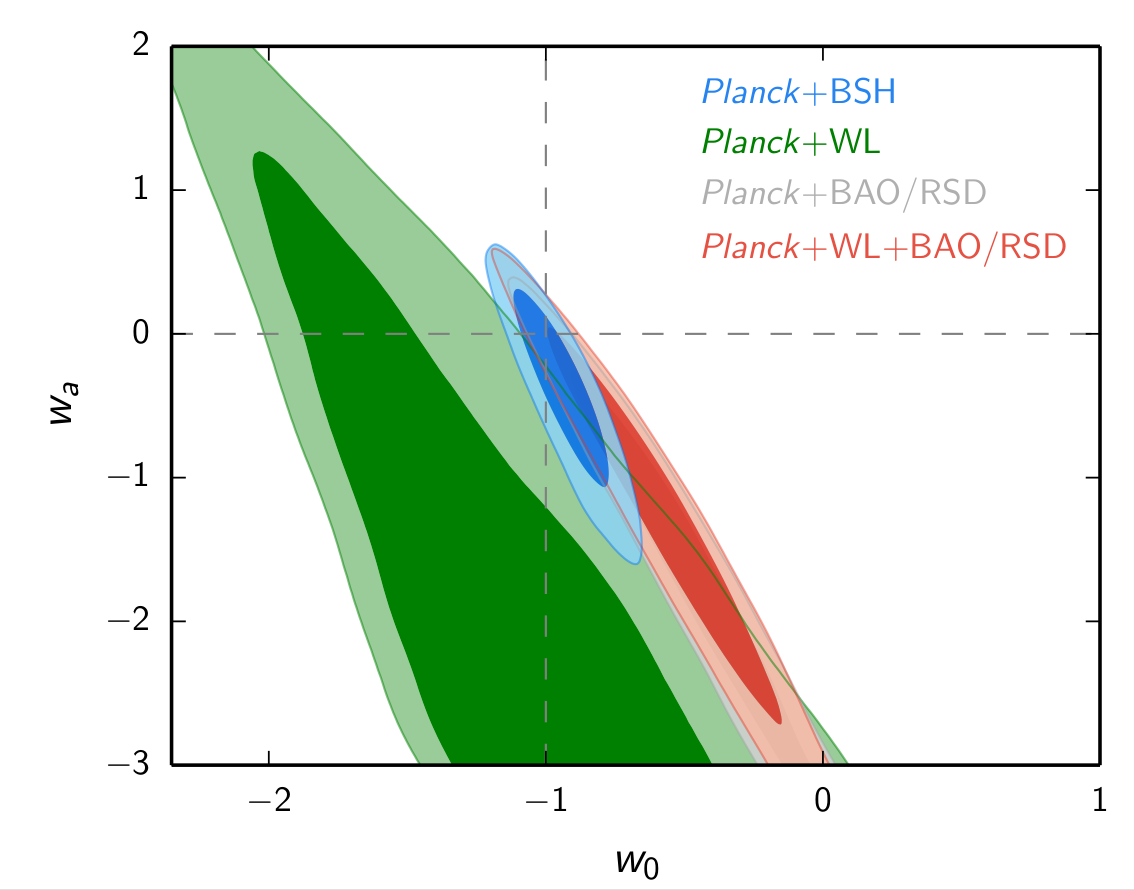
\includegraphics[width=0.8\textwidth,trim={0 3mm 0 0},clip]{./Pictures/w0wa_planck2015.png}
\caption{One- and two- sigma contours of the equation of state of dark energy $w_0,w_a$. The intersection of dashed lines is the cosmological constant. Results obtained from Planck Collaboration 2015 results \cite{2016A&A...594A..14P}.}
\label{fig:w0wa_planck2015}
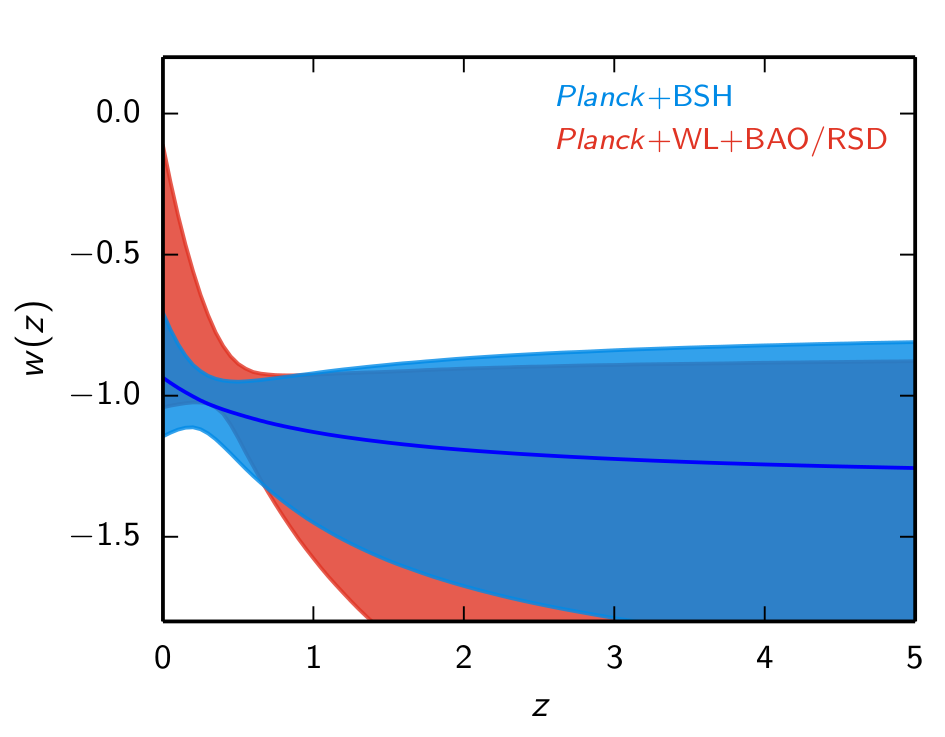
\includegraphics[width=0.8\textwidth]{./Pictures/equationofstate_planck2015.png}
\caption{One-sigma confidence interval of the equation of state of dark energy as a function of redshift $w_{DE}(z)$ and one-sigma confidence interval. Results obtained from Planck Collaboration 2015 results \cite{2016A&A...594A..14P}.}
\label{fig:equationofstate_planck2015}
\end{center}
\end{figure}

\begin{figure}
\begin{center}
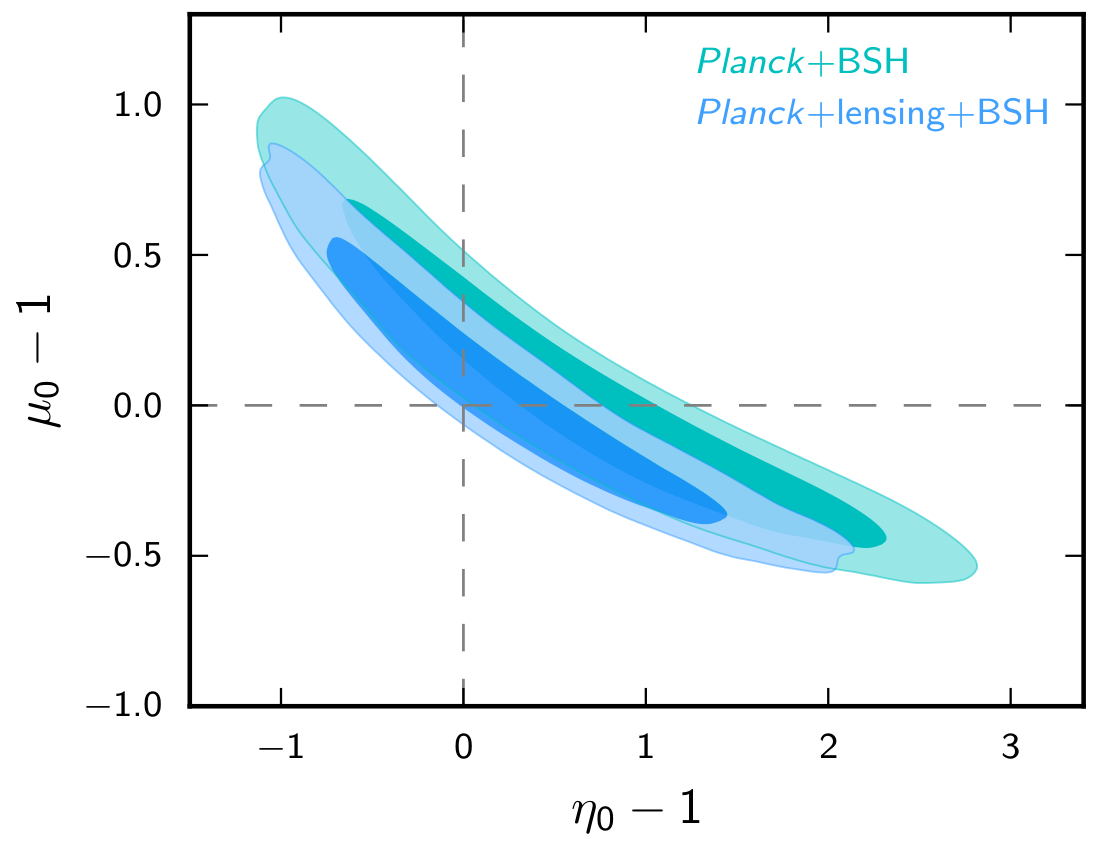
\includegraphics[width=0.8\textwidth]{./Pictures/mg_planck2015.png}
\caption{One- and two- sigma modified gravity potentials at present $\mu_0,\eta_0$. Dashed line is General Relativity plus cosmological constant. Results obtained from Planck Collaboration 2015 results \cite{2016A&A...594A..14P}.}
\label{fig:mg_planck2015}
\vspace*{0.2cm}
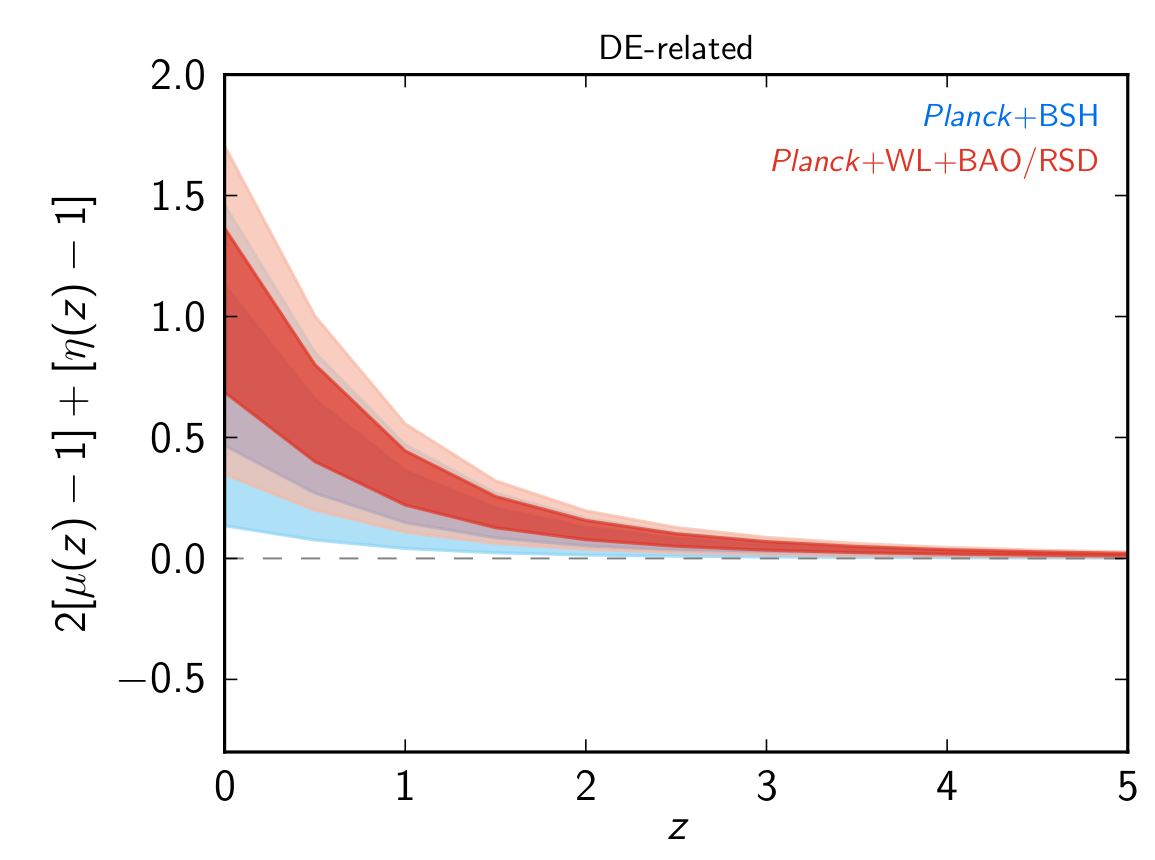
\includegraphics[width=0.8\textwidth]{./Pictures/munu_planck2015.png}
\caption{One- and two- sigma of the sum of the modified gravity potentials. Dashed line is General Relativity plus cosmological constant. Results obtained from Planck Collaboration 2015 results \cite{2016A&A...594A..14P}. }
\label{fig:munu_planck2015}
\end{center}
\end{figure}

Although the Planck Collaboration 2015 results seems to favor cosmological constant as dark energy, Riess et~al. latest direct determination of the Hubble constant using the cosmological distance ladder (parallax-cepheids-SNIa) \cite{2016ApJ...826...56R}, show a discrepancy on the $3\sigma$ level with the Hubble constant measured by Planck Collaboration 2015. If more exotic cosmological scenarios are considered, such as non-flatness, additional species of neutrinos or other models of dark energy are allowed, this tension is relaxed. 
\newline

CFHTLens \& KiDS-450 Collaborations galaxy-shear weak-lensing analysis show tension on the $\Omega_M-\sigma_8$ plane with Planck Collaboration 2013 \cite{2014A&A...571A..16P} and 2015 CMB measurements if a General Relativity plus cosmological constant scenario is considered \cite{2013MNRAS.430.2200K,2017arXiv170303383H}. This tension may be alleviated if other models are considered, such as non-zero curvature and dark energy models \cite{2016arXiv161004606J}. Nevertheless, discrepancies could also be produced by systematic effects \cite{2015PhRvD..92b3003D,2017MNRAS.465.2033J}.
\newline

A weak-lensing analysis by Leauthaud et~al. \cite{2017MNRAS.467.3024L} of CFHTLens \& CMASS data using gg-lensing show a lower signal amplitude that the one predicted measuring the clustering of the lens sample. In addition gg-lensing measurements on the $\Omega_M^0-\sigma_8$ plane have a discrepancy on the $3\sigma$ level with Planck Collaboration 2013 measurements on a cosmological constant scenario. Nevertheless, discrepancies are interpreted in terms of new physics on the astronomy side: halo occupation distribution (HOD) and barionic physics.
\newline

As it has been described, current individual constrains on dark energy are not precise enough to determine which model is the correct explanation of the accelerated expansion of the Universe. Current cosmological model --General Relativity with flat geometry plus cosmological constant (flat-$\Lambda$CDM)--, is in crisis since a tension exists between different probes \cite{2016PDU....12...56B}. Dark energy is one of the possible scenarios to solve this tension, although caution is needed and analysis need to put special attention to systematic analysis. This requires additional probes and redundant measurements of the same physical observable but with different sources of systematic errors.


\section{Alternative probes for Dark Energy: Voids \& Troughs}
Previous cosmological probes were based on the same physical quantity: the anisotropies of the matter density-field although at different moments of the Cosmic History. Whereas CMB measures anisotropies at decoupling, lensing and clustering measure them at present. This anisotropies where originated on primordial density fluctuations\footnote{The current hypothesis suggests that this fluctuations are due to inflation.} that, when matter and radiation decoupled, froze. Then, the over-dense regions of the mater field started to grow by gravitational collapse of the matter, leading the the accretion of the matter contained at the under-dense regions, forming the cosmic  web (see \autoref{fig:2df}). This large under-dense regions of the Universe surrounded by over-dense regions are known as voids.
\begin{figure}
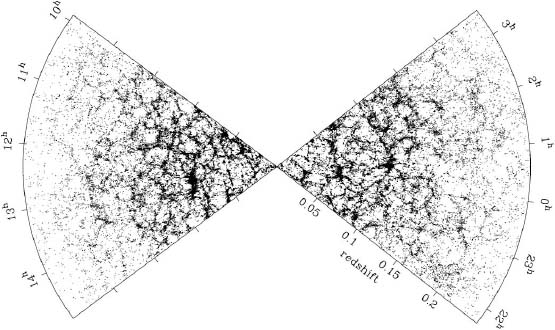
\includegraphics[width=\textwidth]{./Pictures/2df.jpg}
\caption{Large-scale-structure of the Universe. Each dot represents the position of a galaxy. Image credit: 2 Degree Field Survey.}
\label{fig:2df}
\end{figure}
\newline

Since voids have a lower matter content than the average Universe, their gravitational evolution is dominated by dark energy. Thus, void properties are different depending on the dark energy theory that rules the Cosmos. If the abundance of large voids on the Universe is considered, it has been reported that its number increases in $f(R)$ gravity models \cite{2012MNRAS.421.3481L} since the abundance of dark matter halos is altered \cite{2017JCAP...03..012V}. Nevertheless, if the shape of the void is measured, its ellipticity can be used as a probe for the parameters of the equation of state of dark energy \cite{2010MNRAS.403.1392L,0004-637X-754-2-109,PhysRevLett.98.081301,2013PhRvL.111x1103S}, since the structure growth-factor on the line-of-sight has a variation due to
the dark energy content, whereas on the transverse plane, growth-factor is constant. Finally, the radial distribution of matter around the center of a void --known as void profile-- has demonstrated to be different on $f(R)$ theories and General Relativity \cite{2014APh....54...44A,2014arXiv1410.8355C,2015MNRAS.451.4215Z,2015JCAP...08..028B,2016PhRvD..93j3522A,2016PhRvD..94j3524A}. Thus, by simply measuring the void matter profile, constrains on dark energy can be made.
\newline

Nevertheless, the total matter budget of the Universe is composed by both barionic and dark matter, being the presence of the latter only accessible indirectly trough its gravitational effects. As galaxies --mainly composed by barionic matter-- are biased tracers of the underlying dark matter field, its spatial distribution requires a model of assembly of galaxies within dark matter, introducing uncertainties and nuisance parameters on the model. Gravitational light deflection is only sensitive to the total matter field, not needing additional modeling on how barionic and dark matter relate. Thus, gravitational light deflection made by voids constitutes a promising new probe on dark energy.

\chapterimage{head2.png} % Chapter heading image
\chapter{Gravitational Lensing Theory}
\label{ch:theory}
As it has been stated on \autoref{ch:introduction}, the gravitational field acts on the energy-momentum tensor. Thus, massless particles that are carriers of energy --such as photons-- are also affected by gravity, leading to a bending of light rays. The first experimental determination of the gravitational light bending was performed by Dyson et~al. in 1919 \cite{Dyson291}, four years after the publication of General Relativity. On this work, the observed apparent position of stars close to the Sun during a solar eclipse were measured and compared with their positions when the Sun is not in front of them. The positions of the stars where shifted as predicted by General Relativity.
\newline

Dyson et~al. measurement of the gravitational deflection of the light emitted by a background object --a.k.a. source--, relied on the fact that the object that causes of the light deflection --a.k.a. the lens--, can be removed by its own seasonal motion. Nevertheless, this limits the measurement of gravitational light deflection to objects within the Milky Way. The study of the large-scale-structure of the Universe requires the use of extragalactic objects, implying that the object that acts as lens can not be removed, complicating the measurement.
\newline

One specific case of the gravitational light deflection happens when the observer, lens and source are aligned. This problem has cylindrical symmetry and leads to a very specific solution: the Einstein ring (\autoref{fig:einstein_ring}) \cite{2016ApJ...827...51N}. On this configuration, the image of the background galaxy is distorted forming a ring around the lens galaxy, that its located at its center. The size of the ring is determined only by the mass of the lens and the distances of the lens and the source:
\begin{equation}
\theta_E = \sqrt{\frac{4G_NM}{c^2}\frac{d_{LS}}{d_Ld_S}},
\end{equation}
where $G_N$ is Newton's gravitational constant, $M$ the mass of the lens, $d_{LS}$ the lens-source angular diameter distance and $d_L,d_S$ are the angular diameter distance to the lens and the source respectively.
\begin{figure}
\begin{center}
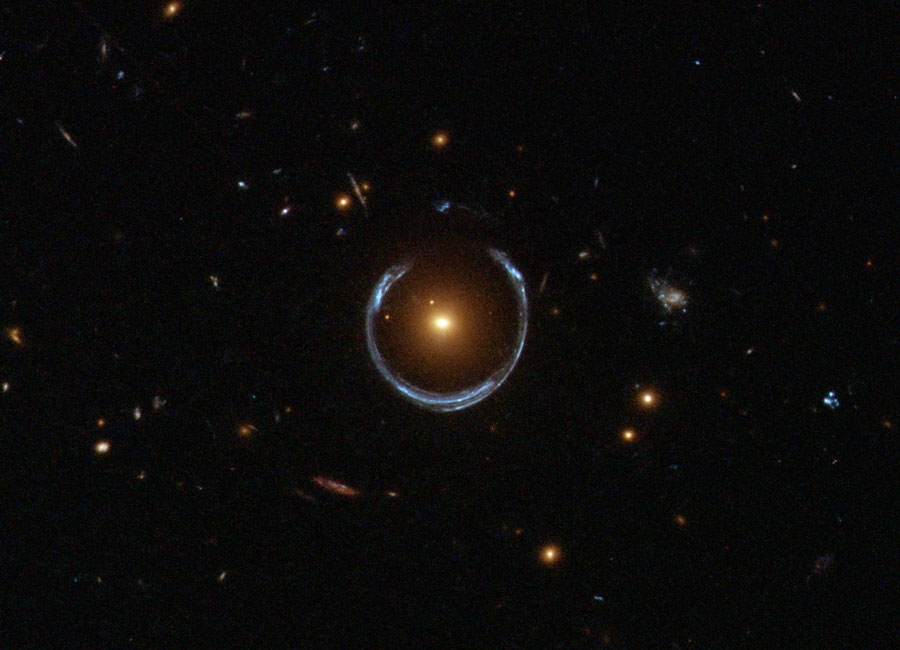
\includegraphics[width=\textwidth]{./Pictures/einstein_ring.jpg}
\caption{Image form the Hubble's Wide Field Camera 3 showing an Einstein ring. Central galaxy is the luminous red galaxy LRG-3-757. The blue annulus is a distant galaxy located behind the LRG. Image credit: NASA.}
\label{fig:einstein_ring}
\end{center}
\end{figure}
\newline

Finding Einstein rings may be a product of serendipity or digging hard on wide-field images \cite{2017arXiv170402744J}. Nevertheless, the probability of finding a system where observer-lens-source are aligned is very small and only a modest number of Einstein rings are known ($\sim20$ on the Dark Energy Survey Science Verification data). A more general solution, where the system is not aligned can be found with the gravitational lens equation and is more useful for cosmology since the statistics grows enormously.

\section{Lens Equation on Gravitational Fields}
Since all the photons emitted by the source are bended coherently by the lens, the axis observer-lens constitute an optical convergent system. Thus a lens equation can be deduced using Geometrical Optics with the deflection angle ($\hat\alpha$) of a light ray --photon trajectory-- given by General Relativity \cite{Weinberg,2001PhR...340..291B,2006glsw.conf.....M,2008ARNPS..58...99H,2041-8205-723-1-L13,Weinberg201387,2015RPPh...78h6901K}:
\begin{equation}
\hat\alpha = \frac{4G_NM}{\xi c^2}.
\label{eq:deflection_angle}
\end{equation}
Here $M$ is the mass of the point-particle (lens hereafter), $G_N$ is Newton's constant, $c$ the speed of light and $\xi$ the closest encounter distance (a.k.a. impact paramenter). Using \autoref{fig:optical_system} as reference and defining $\theta$ as the observed and $\beta$ the real lens-source angle, it can be deduced that
\begin{equation}
\beta = \theta - \frac{D_{ds}}{D_s}\hat\alpha(D_d\theta)=\theta-\alpha(\theta),
\label{eq:lens_equation}
\end{equation}
where $D_{ds},D_s$ and $D_d$ are the source-lens, observer-source and observer-lens comoving distances.
\begin{figure}
\begin{center}
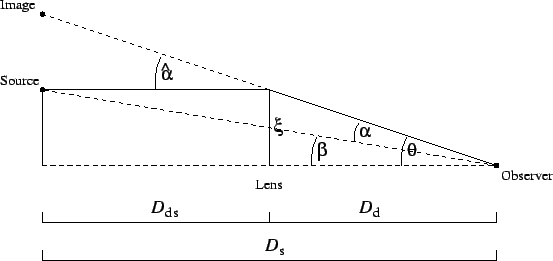
\includegraphics[width=0.9\textwidth]{optical_system.png}
\caption{Optical system of the gravitational lensing caused by a point mass. Solid line is the actual photon trajectory. Dashed lines are the apparent trajectories with and without lensing. The distances $D_s,D_d,D_{ds}$ are expressed in comoving coordinates. }
\label{fig:optical_system}
\vspace{1cm}
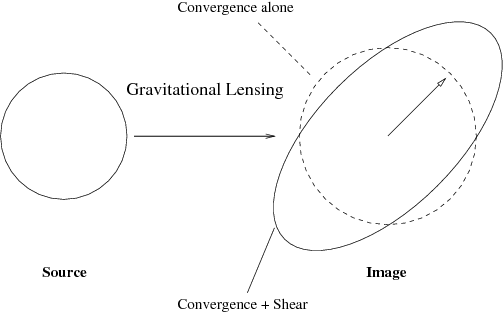
\includegraphics[width=0.9\textwidth]{./Pictures/distortion.png}
\caption{Weak-lensing distortion of an extended spherical object. Convergence leads to an isotropic enlargement, whereas shear produces an elongation/shrink along one axis.}
\label{fig:wl_distortion}
\end{center}
\end{figure}
\newline

Considering now an extended matter distribution, with density $\rho(\vec r)$, where the observer is located at the origin. The position vector can be splitted such that
\begin{equation}
\vec r = r_\parallel \hat r_\parallel + \vec r_\perp,
\end{equation}
where $r_\parallel\hat r_\parallel$ denotes the position on the direction defined by the axis observer-lens (line-of-sight or LoS hereafter) and $\vec r_\perp$ denotes a 2D vector on the plane transverse to the line-of-sight. Thus, the total matter distribution that the photon goes trough from the source to the observer is given by
\begin{equation}
\Sigma(\vec r_\perp,r_\parallel^S) = \int\limits_0^{r_\parallel^S} dr_\parallel\rho(r_\parallel,\vec r_\perp),
\label{eq:surface_density}
\end{equation}
where $\vec r^S$ is the position of the source and the quantity $\Sigma$ is called the surface density. Taking into account the flat-sky approximation\footnote{This approximation is responsible of part of the Planck-CFHTLens/KiDS tension.} --that is, all the transverse planes to LoS are parallel-- and summing to all the lens positions, \autoref{eq:deflection_angle} becomes
\begin{equation}
\hat\vec\alpha(\vec r_\perp,r_\parallel^S) = \frac{4G_N}{c^2}\int d^2\vec r_\perp \Sigma(\vec r_\perp,r_\parallel^S)\frac{\vec r^S_\perp-\vec r_\perp}{|\vec r^S_\perp-\vec r_\perp|^2}.
\end{equation}
This leads to a deflection angle
\begin{equation}
\hat \vec\alpha(\vec r_\perp,r_\parallel^S) = \frac1{\pi}\int d^2\vec r_\perp\kappa(\vec r_\perp,r_\parallel^S)\frac{\vec r^S_\perp-\vec r_\perp}{|\vec r^S_\perp-\vec r_\perp|^2},
\end{equation}
where the convergence ($\kappa$) and critical density ($\Sigma_c$) has been defined such that
\begin{equation}
\kappa(\vec r_\perp,r_\parallel^S) = \frac{\Sigma(\vec r_\perp,r_\parallel^S)}{\Sigma_c} \mbox{ with } \Sigma_c = \frac{c^2}{4\pi G_N}\frac{D_s}{D_dD_{ds}}.
\label{eq:kappa_definition}
\end{equation}
As weak-lensing wide-field surveys start to proliferate, the limit of validity of the flat-sky approximation is being reached \cite{2017arXiv170205301K,2017arXiv170401054L}. A solution without the flat-sky approximation can be found at Kitching et~al. \cite{2016arXiv161104954K}, and adds an additional prefactor that is function of the wavenumber on the power spectrum. Defining the lensing potential as
\begin{equation}
\psi(\vec r_\perp,r_\parallel^S) = \frac1{\pi}\int d^2\vec r_\perp\kappa(\vec r_\perp,r_\parallel^S)\ln|\vec r^S_\perp-\vec r_\perp|,
\end{equation}
the deflection angle can be written as the gradient of the lensing potential on the transverse plane
\begin{equation}
\hat\vec\alpha(\vec r_\perp,r_\parallel^S) = \nabla_\perp\psi(\vec r_\perp,r_\parallel^S)
\end{equation}
and the convergence as its laplacian,
\begin{equation}
\kappa(\vec r_\perp,r_\parallel^S)=\frac{1}{2}\nabla^2_\perp\psi(\vec r_\perp,r_\parallel^S).
\end{equation}
Thus, the lens equation from \autoref{eq:lens_equation} results
\begin{equation}
\vec\beta = \vec\theta-\nabla_\perp\psi(\vec r_\perp,r_\parallel^S).
\label{eq:lens_equation_2d}
\end{equation}
Taking into account the definition of the lensing potential, it can also be written in terms of the Newtonian gravitational potential ($\Phi$):
\begin{equation}
\psi(\vec r_\perp,r_\parallel^S) = \frac{D_{ds}}{D_sD_d}\frac{2}{c^2}\int dr_\parallel^S\Phi(D_d\vec r_\perp,r_\parallel^S).
\end{equation}
Thus, gravitational lensing is a direct probe for the underlying gravitational field.

\section{Weak Gravitational Lensing}

In addition to the change in the observed position of the source, considering no absorption nor emission of photons between the source and the observer, Liouville's theorem implies that the surface brightness of the source ($I_S$)is conserved,
\begin{equation}
I_S(\vec r_\perp) = I_S[\vec\beta(\vec r_\perp)].
\end{equation}
Considering the weak-field regime, the lensing map can be linearized such that
\begin{equation}
I_S(\vec r_\perp)=I_S[\vec\beta_0+\mathcal{J}(\vec r_{\perp 0})(\vec r_\perp-\vec r_{\perp0})],
\end{equation}
where $\mathcal{J}(\vec r_\perp)$ is the jacobian matrix. By the integration-by-substitution theorem of calculus, the integral of the surface brightness at the lensed and un-lensed coordinate systems are related by
\begin{equation}
\int I_S(\vec\beta)d\vec\beta = \det(\mathcal{J})\int I_S[\vec\beta(\vec r_\perp)]d\vec r_\perp,
\end{equation}
where $\det(\mathcal{J})$ denotes the determinant of the jacobian matrix. Thus, defining the luminosity of an extended object as the integral of its surface brightness, the luminosity for the cases with and without gravitational lensing ($L_\mu,L_0$ respectively) are related by
\begin{equation}
L_\mu = \frac{1}{\det(\mathcal{J})}L_0 = \mu L_0,
\end{equation}
where $\mu$ is called the magnification factor and is defined as de inverse of the determinant of the jacobian matrix of the lensing map.
\newline

Taking into account that the jacobian matrix is given by $\mathcal{J}=(\hat n_\perp\cdot\nabla_\perp)\vec\beta$ with $\hat n_\perp$ a unit vector on the plane transverse to LoS, by \autoref{eq:lens_equation_2d} the jacobian can be expressed as
\begin{equation}
\mathcal{J} = (\hat n_\perp\cdot\nabla_\perp)\vec r_\perp-\mathcal{J} = (\hat n_\perp\cdot\nabla_\perp)\nabla\psi,
\end{equation}
resulting finally 
\begin{equation}
\mathcal{J}(\vec r_\perp) = \left(\delta_{ij}-\frac{\partial^2\psi}{\partial r_i\partial r_j}\right)=\left( \begin{array}{c c}1-\kappa-\gamma_1 & -\gamma_2\\-\gamma_2 & 1-\kappa+\gamma_1\end{array} \right).
\label{eq:jacobian}
\end{equation}
Here $\kappa$ is the convergence, an isotropic shape distortion and $\gamma_1,\gamma_2$ is the shear, an elongation/shrink on the shape along one of the axis (\autoref{fig:wl_distortion}).
\newline

Taking into account the Born approximation --that is, the light rays of a source galaxy are deflected by only one lens--, the derivatives of the previous equation can be evaluated on the unlensed coordinates.

\subsection{Magnification}
As it has been demonstrated in the previous section, gravitational lensing increases the observed luminosity on an extended object \cite{1989Sci...245..824B,1992RvMA....5..259B,1992LNP...406..345B,1995A&A...303..643B,1995AIPC..336..307B} such that $L_\mu = \mu L_0$ with 
\begin{equation}
\mu = \frac1{(1-\kappa)^2+\gamma_1^2+\gamma_2^2}\simeq 1+2\kappa,
\label{eq:mu_definition}
\end{equation}
where on the last step it has been used that $1\gg\kappa\gg\gamma$. Taking into account the definition given at \autoref{eq:kappa_definition}, the convergence suffered by the photons emitted by a source located on the sky direction $\hat n$ and redshift $z$ is given by
\begin{equation}
\kappa(\hat n,z) = \frac{1}{2}\frac{\Sigma(\hat n,z)}{\Sigma_c}.
\end{equation}
Using the definition given at \autoref{eq:surface_density} and the poisson equation for the gravitational field this leads to
\begin{equation}
\kappa(\hat n,z) = \int\limits_0^zdz'\frac{r(z')[r(z)-r(z')]}{r(z)}\nabla_\perp\Phi(\hat n,z'),
\label{eq:kappaphi}
\end{equation}
where $r(z)$ is the comoving distance at redshift $z$ and $\Phi$ the gravitational potential. Expressing now the gravitational potential as an homogeneus therm plus a perturbation ($\Phi = \bar\Phi+\delta_\Phi$), the previous equation can be expressed as a funcion of the matter density contrast ($\delta_M$)
\begin{equation}
\nabla^2\Phi(\hat n,z) = \nabla^2\delta_\Phi(\hat n,z) = 4\pi Ga^2\bar\rho\delta_M(\hat n,z),
\label{eq:kappadeltam}
\end{equation}
where $a=1/(1+z)$ is the scale factor and $\bar\rho$ is the average density. This leads finally to \cite{PhysRevD.76.103502,PhysRevD.77.063526}
\begin{equation}
\kappa(\hat n,z) = \frac{3H_0\Omega_M(z)}{2c^2}\int\limits_0^zdz'\frac{r(z')[r(z)-r(z')]}{(1+z')r(z)}\delta_M(\hat n,z).
\label{eq:kappadeltam}
\end{equation}
The convergence is the physical observable of magnification and it traces the matter density on the direction of line of sight whereas shear probes the matter on the transverse direction. This makes magnification and shear complementary measurements of the same phenomena. The dependence of magnification is usually split into two pieces: the lensing kernel,
\begin{equation}
\mathcal{K}(z) = \frac{r(z')[r(z)-r(z')]}{(1+z')r(z)}.
\end{equation}
and the matter density contrast ($\delta_M$). The lensing kernel contains only geometrical information and, for a given set of cosmological parameters, it is fixed. On the other side, the matter density contrast is sensitive to the growth of structure in the Universe. We see that weak lensing is both a geometrical and growth of structure probe of cosmology.
\newline

The convergence of the foreground sample can be probed tracing the three effects that it produces on the background sample:
\begin{itemize}
\item {\bf Change of the observed density:} The increase of the observed luminosity of the galaxies allows to see sources that if there were no lensing, would be below our observational threshold nearby the location of the lenses. At the same time, an stretching of the solid angle behind the lenses causes a drop in the number density. This two effects compete between them and which one is over the other depends on the slope of the number counts of the sources. Thus, at the neighbourhood of the lenses, a change of the number density respect to the average is produced. This is known as number-count magnification.
\item {\bf Shift on the observed magnitude:} Since the increase of luminosity due to gravitational lensing is a short range effect, a shift on the observed magnitudes may be detected nearby the positions of the lenses. This requires, in principle, the knowledge of the unlensed magnitude of the sources. Nevertheless, although galaxies have a large variety of magnitudes, it can be assumed that, they are randomly distributed. Thus shifts on the magnitudes respect to the average can be detected.
\item {\bf Size enlargement:} All the effects above are a consequence of the conservation of surface brightness and the size enlargement of the sources. This enlargement can be statistically measured despite the fact that the unlensed size is not known. Nevertheless, since galaxies have a large variety of shapess and size that is strongly related to its evolution and age, no homogeneity assumption can be made and require the use of empirical relations like the {\it fundamental plane} \cite{2003AJ....125.1866B,2041-8205-780-2-L16}.
\end{itemize}

Traditionally all these probes have been used independently, but the ideal scenario would be a three-way combination that may lead to a cancellation or better estimation of systematic errors.
\newline

As it has been mentioned before, the knowledge of the unlensed properties of the sources is physically impossible. Thus, all the observable quantities must be formulated in terms of changes of its variation respect the ensemble average with the distance to the lenses. The statistical way to do this is through the two-point angular correlation-function. This method provides a measurement of the average convergence profile of the lenses ($\kappa(\theta)$) as a function of its angular distance $\theta$ of a point to the lens.

\subsubsection{Estimation of $\kappa(\theta)$ with the number counts technique}
The two-point angular cross-correlation between positions of galaxies in the sample lens ($L$) and in the source sample ($S$) is defined as \cite{PhysRevD.77.023512,}
\begin{equation}
\omega_{LS}(\theta) = \langle\delta_O(\hat n,z_L,f_\mu)\delta_O(\hat n',z_S,f_\mu)\rangle_{\theta}.
\label{eq:2pacfmagnification}
\end{equation}
Where $\delta_O(\hat n,z_L,f_\mu)$ is the observed galaxy density-contrast on the sky direction $\hat n$ and redshift $z_L$ with flux limit $f_\mu$. $\omega_{LS}$ is not zero, since due to magnification galaxies beyond the observable threshold will appear nearby the lenses introducing a non-uniform distribution of galaxies. Thus the observed galaxy density contrast can be expressed as
\begin{equation}
\delta_O(\hat n,z,f_\mu) = \delta_g(\hat n,z)+\delta_\mu(\hat n,z,f_\mu),
\end{equation}
where $\delta_g$ is the intrinsic galaxy-density contrast (that is, without magnification) and $\delta_\mu$ is the density contrast due to magnification. Thus \autoref{eq:2pacfmagnification} becomes
\begin{equation}
\omega_{LS}(\theta) = \langle\delta_g(z_L)\delta_g(z_S)\rangle+\langle\delta_g(z_L)\delta_\mu(z_S)\rangle+\langle\delta_\mu(z_L)\delta_g(z_S)\rangle+\langle\delta_\mu(z_L)\delta_\mu(z_S)\rangle.
\label{eq:4t}
\end{equation}
Taking into account that $0<z_L<z_S$, and that the lens and the source sample are well separated in redshift, the only non vanishing term is
\begin{equation}
\omega_{LS}(\theta) = \langle\delta_g(\hat n,z_L)\delta_\mu(\hat n,z_L,f_\mu)\rangle_\theta.
\end{equation}
Let define the magnification density contrast on the sky direction $\hat n$ as 
\begin{equation}
\delta_\mu(\hat n,z,f_\mu) = \frac{N_\mu(\hat n,z,f_\mu)}{N_0(\hat n,z,f_0)}-1,
\end{equation}
where $N_0(\hat n,z,f_0)$ is the un-lensed cumulative number counts of sources located at redshift $z$, that is, the number of sources with observed flux greater than the threshold $f_0$. Conversely, $N_\mu(\hat n,z,f_\mu)$ is the lensed cumulative number counts affected by magnification.
\newline

Magnification by gravitational lenses increases the observed flux of background objects  allowing to see fainter sources by an amount $f_\mu = f_0/\mu$. At the same time, it stretches the solid angle behind the lenses, reducing the surface density of sources an amount $N_\mu = N_0/\mu$, which translates into the density contrast as:
\begin{equation}
\delta_\mu(\hat n,z,f_\mu) = \frac{N_\mu(\hat n,z,f_\mu)}{\mu N_\mu(\hat n,z,\mu f_\mu)}-1.
\label{eq:magnification_density_contrast}
\end{equation}
The cumulative number counts can be locally parametrized as a power law
\begin{equation}
N_\mu(\hat n,z,f_\mu) = A\left(\frac{f_\mu}{f_*}\right)^{\alpha(f_\mu)},
\end{equation}
where $A,f_*$ are constant parameters and $\alpha(f_\mu)$ a function of the flux limit. Substituting this into \autoref{eq:magnification_density_contrast}
\begin{equation}
\delta_\mu(\hat n,z,f_\mu) = \mu^{\alpha(f_\mu)-1}-1.
\end{equation}
Taking into account the weak-lensing approximation $\mu\simeq 1+2\kappa$ along with \autoref{eq:mu_definition} and translating from fluxes to magnitudes this results
\begin{equation}
\delta_\mu(\hat n,z,m) = 2\kappa(\hat n,z)[\alpha(m)-1]
\end{equation}
with
\begin{equation}
\alpha(m) = 2.5\frac{d}{dm}\left[\log N_\mu(m)\right].
\label{eq:alpha}
\end{equation}
Thus \autoref{eq:2pacfmagnification} becomes
\begin{equation}
\omega_{LS}(\theta) = 2[\alpha(m)-1]\langle\delta_g(\hat n,z_L)\kappa(\hat n',z_S)\rangle_\theta = [\alpha(m)-1]2\kappa(\theta),
\label{eq:kappa_nc}
\end{equation}
where $\kappa(\theta)$ is the convergence profile of the selected lenses.

\subsubsection{Estimation of $\kappa(\theta)$ with magnitude-shift magnification technique}
The magnitude-position-angular correlation function between the lens sample ($L$) and the source sample ($S$) is defined as
\begin{equation}
\varphi_{LS}(\theta) = \langle\delta_g(z_L,\hat n)\delta_m(z_S,\hat n')\rangle_\theta.
\label{eq:mpacf}
\end{equation}
Where, as on  the last section $\delta_g (z,\hat n)$ is the galaxy density contrast at redshift $z$ on the sky direction $\hat n$ and $\delta_m$ is the magnitude shift\footnote{Do not confuse with $\delta_M$, the matter density contrast.}, defined as
\begin{equation}
\delta_m(z,\hat n) = m_\mu(\hat n,z)-m_0(\hat n,z),
\end{equation}
where $m_\mu$ is the lensed magnitude and $m_0$ the unlensed magnitude. Taking into account that, as it has been demonstrated previously,
\begin{equation}
f_\mu(\hat n,z) = \mu(\hat n,z)f_0(\hat n,z) \Leftrightarrow m_\mu(\hat n,z)-m_0(\hat n,z) = -2.5\log\mu(\hat n,z),
\end{equation}
where on the last step it has been converted from fluxes to magnitudes. Thus, taking into account that
\begin{equation}
\log(\mu) \simeq \log(1+2\kappa)\simeq 2\kappa,
\end{equation}
the \autoref{eq:mpacf} results finally
\begin{equation}
\varphi_{LS}(\theta)= -5\langle\delta_g(\hat n,z_L)\kappa(\hat n',z_S)\rangle = -5\kappa(\theta),
\end{equation}
where $\kappa(\theta)$ is the convergence profile of the lenses.
\newline

Nevertheless, reddening by the inter-galactic medium  can also produce --unlike gravitational lensing-- wavelength-dependent magnitude-shifts. Thus, the lensed-plus-reddened fluxes are given by
\begin{equation}
f_\mu(\hat n,z,\lambda_\eta) = \mu(\hat n,z)f_0(\hat n,z)e^{-\tau(\lambda_\eta)},
\end{equation}
that converted to magnitudes results in
\begin{equation}
m_\mu(\hat n',z,\lambda_\eta)-m_0(\hat n',z,\lambda_\eta)=-2.5\log\mu+\frac{2.5}{\ln 10}\tau(\lambda_\eta),
\end{equation}
where $\tau(\lambda_\eta)$ is the optical depth at the wavelength $\lambda_\eta$. The dust and the lensing components can be disentangled by defining the color-excess angular correlation function ($E^{\eta\nu}$) between two-wavelengths $\lambda_\eta,\lambda_\nu$,
\begin{equation}
E^{\eta\nu}_{LS}(\theta) = \langle\delta_g(\hat n,z_L)[m_\mu(\hat n',z_S,\lambda_\eta)-m_\mu(\hat n',z_S,\lambda_\nu)]\rangle_\theta.
\end{equation}
Since gravitational lensing is acromatic, the only dependence with the wavelength comes from the extinction law
\begin{equation}
E^{\eta\nu}_{LS}(\theta)=\frac{2.5}{\ln 10}\langle\delta_g(\hat n,z_L)[\tau(\hat n',z_S,\lambda_\eta)-\tau(\hat n',z_S,\lambda_nu)]\rangle.
\end{equation}

Modeling the wavelength dependence of the optical depth as \cite{2010MNRAS.405.1025M}
\begin{equation}
\tau_\eta = \tau(\lambda_\eta) = \tau_V\left(\frac{\lambda_V}{\lambda_\eta}\right)^\gamma,
\end{equation}
where $\tau_V$ is the optical depth at the $V$-band filter, $\lambda_V$ is the wavelength of the $V$-band filter and $\gamma\sim 1$ is a constant parameter. Thus, the color-excess cross-correlation results finally
\begin{equation}
E^{\eta\nu}_{LS}(\theta)=\lambda_V(\lambda_\eta^{-1}-\lambda_\nu^{-1})\frac{2.5}{\ln 10}\langle\delta_g(\hat n,z_L)\tau_V(\hat n',z_S)\rangle.
\end{equation}
At a wide field survey with several broad-band band-pass filters the scale dependence of the optical depth, $\tau_V(\hat n,z_S)$ can be constrained.

\subsection{Shear}
From the Jacobian of the lensing map, it can be deduced that the transformation is not isotropic producing an elongation along one of the axis $(r_1,r_2) = \vec r_\perp$. Thus, an intrinsically round galaxy is seen as elliptical. On the case of elliptical galaxies, statistically they present a null global ellipticity\footnote{If they do not present null ellipticity it is a systematic effect known as intrinsic alignment.}. From the definition of \autoref{eq:jacobian}, the shear components are given by:
\begin{equation}
\gamma_1(\vec r_\perp) = -\frac{1}{2}\left(\frac{\partial^2\psi}{\partial r_1^2}-\frac{\partial^2\psi}{\partial r_2^2}\right)\mbox{ and }\gamma_1(\vec r_\perp) = -\frac{\partial^2\psi}{\partial r_1\partial r_2}.
\end{equation}
The shear fields $\gamma_1,\gamma_2$ can be expressed as Fourier series such that:
\begin{equation}
\tilde \gamma_{1,2}(\vec k_\perp) = \int \gamma_{1,2}(\vec r_\perp)e^{-i\vec k_\perp\cdot\vec r_\perp}d^2\vec r_\perp
\end{equation}
and
\begin{equation}
\gamma_{1,2}(\vec r_\perp) = \frac{1}{(2\pi)^2}\int \tilde\gamma_{1,2}(\vec k_\perp)e^{i\vec k_\perp\cdot\vec r_\perp}d^2\vec k_\perp.
\end{equation}
Expressing the differential equation at the Fourier space with the usual approach $\partial/\partial r_1\rightarrow ir_1$ it leads to
\begin{equation}
\gamma_1(\vec k_\perp) = \frac{1}{2}(r_1^2-r_2^2)\tilde\psi(\vec k_\perp)\mbox{ and }\gamma_2(\vec k_\perp) = \frac{1}{2}r_1r_2\vec \psi(\vec r_\perp)
\end{equation}

Considering a plane-wave perturbation of the lensing potential, it is useful to align the axis of the perturbation with those of the shear field such that
\begin{equation}
\tilde \gamma_E(\vec k_\perp) = \cos(2\phi_{\vec k_\perp})\tilde \gamma_1(\vec k_\perp)+\sin(2\phi_{\vec k_\perp})\tilde \gamma_2(\vec k_\perp)
\end{equation}
and
\begin{equation}
\tilde \gamma_B(\vec k_\perp) = \cos(2\phi_{\vec k_\perp})\tilde \gamma_1(\vec k_\perp)-\sin(2\phi_{\vec k_\perp})\tilde \gamma_2(\vec k_\perp).
\end{equation}
Resulting finally that
\begin{equation}
\tilde\gamma_E(\vec k_\perp) = \vec k_\perp^2\tilde\psi(\vec k_\perp)\mbox{ and }\tilde\gamma_B(\tilde k_\perp) = 0
\end{equation}
The fact that $\gamma_B$ is zero, constitutes a necessary (but not sufficient) proof for the lack of systematic effects on any shear measurement.
\newline

Reaching this point, two kinds of two-point statistics can be build: the point-shear\footnote{This is usually called galaxy-galaxy- (or gg-) lensing.} and the shear-shear two-point angular-correlation functions. From this two, we will only focus to gg-lensing due to its direct connection to magnification.

\subsubsection{The gg-lensing.}
Defining $\tilde\epsilon$ as the observed ellipticity, taking into account shear distortions it can be expressed as:
\begin{equation}
\tilde\epsilon = \tilde\epsilon_i + \tilde\gamma,
\end{equation}
where $\tilde\epsilon_i$ is the intrinsic ellipticity of the galaxy. As stated previously, without loss of generality, shear coordinates can be rotated.  Thus, let define the tangential shear $\gamma_t$ as
\begin{equation}
\gamma_t = -[\cos(2\phi_{\vec k_\perp})\tilde \gamma_1(\vec k_\perp)+\sin(2\phi_{\vec k_\perp})]\tilde \gamma_2(\vec k_\perp) = -\gamma_E.
\end{equation}
On the new coordinates, this leads to
\begin{equation}
\epsilon = \epsilon_i+\gamma_E,
\end{equation}
where $\tilde\epsilon,\tilde\epsilon_i$ are the ellipticity on the new coordinates. Let $p(\epsilon)$ the distribution of ellipticity of the sources.  At the small distortion regime, assuming that ellipticity is isotropic, it follows that
\begin{equation}
p(\epsilon) = p(\epsilon_i)+\gamma_t\cos2\phi\frac{\partial p(\epsilon)}{\partial \epsilon}.
\end{equation}
Here $\phi_{\vec k_\perp}$ is the angle of orientation of the principal axis of the galaxy. Integrating over all the ellipticity, they can be translated to orientation angle,
\begin{equation}
p(\phi) = \frac{2}{\pi}\left[1-\langle\gamma_t\rangle\cos2\phi\left\langle\frac1{\epsilon}\right\rangle\right].
\end{equation}
Thus, measuring the ellipticity --or orientation angles--, shear E-modes can be measured, probing directly the underlying lensing potential.
\newline

Tangential shear can be estimated to be
\begin{equation}
\langle\gamma_t\rangle = -\frac{\Delta\Sigma}{\Sigma_c},
\end{equation}
with
\begin{equation}
\Delta\Sigma = \bar\Sigma(\theta)-\Sigma(\theta),
\end{equation}
where $\bar\Sigma(\theta)$ denotes the average surface density on an disk of angular size $\theta$. Thus the tangential shear can be related to the convergence profile as
\begin{equation}
\langle\gamma_t\rangle=-[\bar\kappa(\theta)-\kappa(\theta)].
\end{equation}
\newline

The last equation demonstrates that gg-lensing and magnification are produced by the same physical effect. Nevertheless, they have different systematic effects. This can be exploited in order to produce accurate and reliable cosmological measurements. 

\section{Theoretical expressions for $\kappa(\theta)$}
As it has been stated on the previous section, the convergence profile  is one of the physical observables for both magnification and gg-lensing. Thus, in order to connect the measurements with a cosmological model, its dependence on the cosmological parameters must be provided. Depending on the nature of the lenses considered --that is, whether the lenses are galaxies, voids, clusters or troughs--, the approach may differ.
\newline

On this section, the solutions for galaxies and voids is calculated. A simple solution for troughs can be found on Gruen et~al. \cite{2016MNRAS.455.3367G}.
\newline

The simplest solution for the convergence profile is for a sample of galaxies. Taking into account the definition of $\kappa$
\begin{equation}
\kappa(\theta) = \langle\delta_g(\hat n,z_L)\kappa(\hat n',z_S)\rangle_\theta,
\end{equation}
if a linear, constant and redshift-independent galaxy-bias ($b_L$) is considered, a relation between the galaxy density contrast $\delta_g$ and matter density contrast $\delta_M$ can be established:
\begin{equation}
\delta_g(\hat n,z_L) = b_L\delta_M(\hat n,z_L).
\end{equation}
Thus, the convergence profile is given by
\begin{equation}
\kappa(\theta) = b_L\langle\delta_M(\hat n,z_L)\kappa(\hat n',z_S)\rangle_\theta.
\end{equation}
If it is considered that the convergence field $\kappa(\hat n)$ can be expressed also as a function of the matter density contrast by \autoref{eq:kappadeltam} and \autoref{eq:kappaphi}:
\begin{equation}
\kappa(\theta) = b_L\left\langle\delta_M(\hat n,z_L)\left[\int\limits_0^zdz'\frac{r(z')[r(z)-r(z')]}{r(z)}4\pi Ga^2\bar\rho\delta_M(\hat n,z)\right]\right\rangle.
\end{equation}
This leads finally to \cite{2003A&A...403..817M}:
\begin{eqnarray}
&\kappa(\theta)=\frac{3H_0^2\Omega_M^0}{2c^2}\int\limits_0^\infty dz'_L\frac{\phi_L(z'_L)}{1+z'_L}\int\limits_{z'_L}^\infty dz'_S\phi_S(z'_S)\frac{r(z'_L)[r(z'_S)-r(z'_L)]}{r(z'_S)}\times\label{eq:omega0}\\
&\int\limits_0^\infty\frac{dkk}{2\pi}P_M(k,z'_L)J_0[k\theta r(z'_i)],\nonumber
\end{eqnarray}
where $\phi_L,\phi_S$ are the redshift distributions of the lens and source sample respectively, $P_M$ the matter power spectrum of the lens sample and $J_0$ is the zero-th order Bessel function.
\newline

The calculation of the convergence profile for a void needs to assume a void profile. A solution on General Relativity for voids can be found at \cite{2008JCAP...04..003G,2016MNRAS.455.1246F,2016MNRAS.462.1882K}, based on the LTB metric,
\begin{equation}
\delta(r_v) = \delta_0g(a)\left(1-\frac{2}{3}\frac{r_v^2}{r_0^2}\right)\exp\left(-\frac{r_v^2}{r_0^2}\right),
\end{equation}
where $r_v$ is the radial comoving distance {\bf on the system of coordinates centered at the void}, $r_0$ the radial size of the void, $\delta_0$ the central underdensity and $g(a)$ the growth factor {\bf not normalized at present}. On the system of coordinates centered on the observer and considering non-spherical voids, this leads to the Kovacs \& Garcia-Bellido void-profile (KGB):
\begin{equation}
\delta_{KGB}(\theta,z) = \delta_0g(a)\left[1-\frac{2}{1+2q^2}\left(\frac{r_\parallel^2}{r_0^2}+\frac{q^2r_\perp^2}{r_0^2}\right)\right]\exp\left[-\left(\frac{r_\parallel^2}{q^2r_0^2}+\frac{r_\perp^2}{r_0^2}\right)\right],
\label{eq:kgb}
\end{equation}
where $q^2=1-e^2$ with $e$ the ellipticity of the void and
\begin{eqnarray}
&r_\parallel=r(z)\cos\theta -r(z_v)\\
&r_\perp=r(z)\sin\theta.
\end{eqnarray}
Here $r(z)$ is the radial comoving distance at redshift $z$, whereas $z_v$ is the redshit of the center of the void and $\theta$ the angular separation form the center of the void. From \autoref{eq:kgb} and \autoref{eq:kappa_definition}, the convergence profile around a single void can be obtained:
\begin{equation}
\kappa(\theta) = \frac{1}{2}\frac{\Sigma_{KGB}(\theta)}{\Sigma_c},
\label{eq:kappakrause}
\end{equation}
where the surface density is given by
\begin{equation}
\Sigma_{KGB}(\theta) = \int\limits_0^\infty dz'\bar\rho_M(z')[\delta_{KGB}(\theta,z')+1].
\end{equation}
Here the $\bar\rho_M(z')$ is the matter average density of the Universe at redshift $z'$, given by
\begin{equation}
\bar\rho(z') = \frac{\Omega_M^0\rho_c}{(1+z')^3}
\end{equation}
with $\rho_c$ the critical energy density of the Universe.
\chapterimage{head2.png} % Chapter heading image
\chapter{The Dark Energy Survey}
\label{ch:DES}

The Dark Energy Survey (DES) \cite{2005astro.ph.10346T} is a $grizY$ photometric galaxy-survey that has as main scientific goal to shed light on the nature of the Dark Energy. DES uses four probes to unravel the nature of Dark Energy: the number of clusters as a function of redshift, the measurement of the scale of the baryon acoustic oscillations (BAO), the weak gravitational lensing of galaxies and the measurement of the Hubble diagram with type Ia Supernovae (SNIa). By the end of five years of observations, DES will cover 5000 deg$^2$ of the Southern Hemisphere up to magnitude $i<24.0$ at the $10\sigma$ detection level. Taking this into account, this survey is expected to measure 10000 clusters up to redshift 1.0, 200 million galaxy-shapes for weak-lensing (with $z<1$), 300 million galaxies for BAO ($z<1.4$) and 3000 SNIa up to redshift 1.0. The power of DES resides on the combination of all the probes breaking degeneracies on the cosmological parameter phase-space leading to a precision better than the 5\% on the parameters $w_0$ and $\Delta w_a<0.2$ on the equation of state of the Dark Energy.
\newline

DES is an international collaboration formed by about 500 scientists from more than 20 institutions from: USA, Spain, UK, Brazil, Germany and Switzerland. The Collaboration has built a very sensitivity camera, DECam (see \autoref{fig:decam} and \autoref{fig:cerrotololo}), that has been mounted at the 4-m Victor M. Blanco Telescope\footnote{This is the same telescope where Schmidt and Perlmutter performed some of the observations leading to the Nobel Prize in 2010 for the discovery of Dark Energy.} at the Cerro Tololo Inter-American Observatory (CTIO), located at La Serena (Chile).

\section{The DECam}
The DECam (Dark Energy Camera), is the main instrument of the experiment. It is composed mainly by:
\begin{itemize}
	\item The 570 megapixel focal plane, formed by 70 CCDs.
    \item Low-noise readout electronics.
    \item Wide-field optical corrector, producing 3 deg$^2$ field of view.
    \item Filter and shutter system.
    \item Hexapod for stability.   
\end{itemize}
Since DES is going to observe very high redshifted galaxies, the used CCDs have been specifically designed at Lawrence Berkeley National Laboratory to detect red light. In order to do so, these CCDs are ten times thicker --250 $\mu m$-- than conventional ones\footnote{Sensitivity to long wavelengths is increased when passing trough more silicon.}. This results in a quantum efficiency $>$80\% on the 600-950 nm range, $>$60\% on the 400-600 nm and $>$50\% on the 900-1000 nm. The DECam focal plane consist of the following types of CCDs:
\begin{itemize}
\item Science array: formed by 62 CCDs with $2048\times 4096$ pixels. Each pixel is $15\mu m$ of side that, at the prime focus fot the  Blanco Telescope, results on 0.27 arc-seconds on the sky.
\item Four $2048\times2048$ guider CCDs.
\item Eight $2048\times 2048$ focus and alignment CCDs.
\end{itemize}
To minimize the noise and dark currents due to the electronic system, DECam operates on an environment cooled by liquid nitrogen at 180 K and a vacuum of $\sim 10^{-9}$ atm. The whole readout process takes 17 seconds (about the same slewing-time of the telescope). Readout electronic boards were produced and designed in Spain at CIEMAT and IFAE.
\begin{figure}
\begin{center}
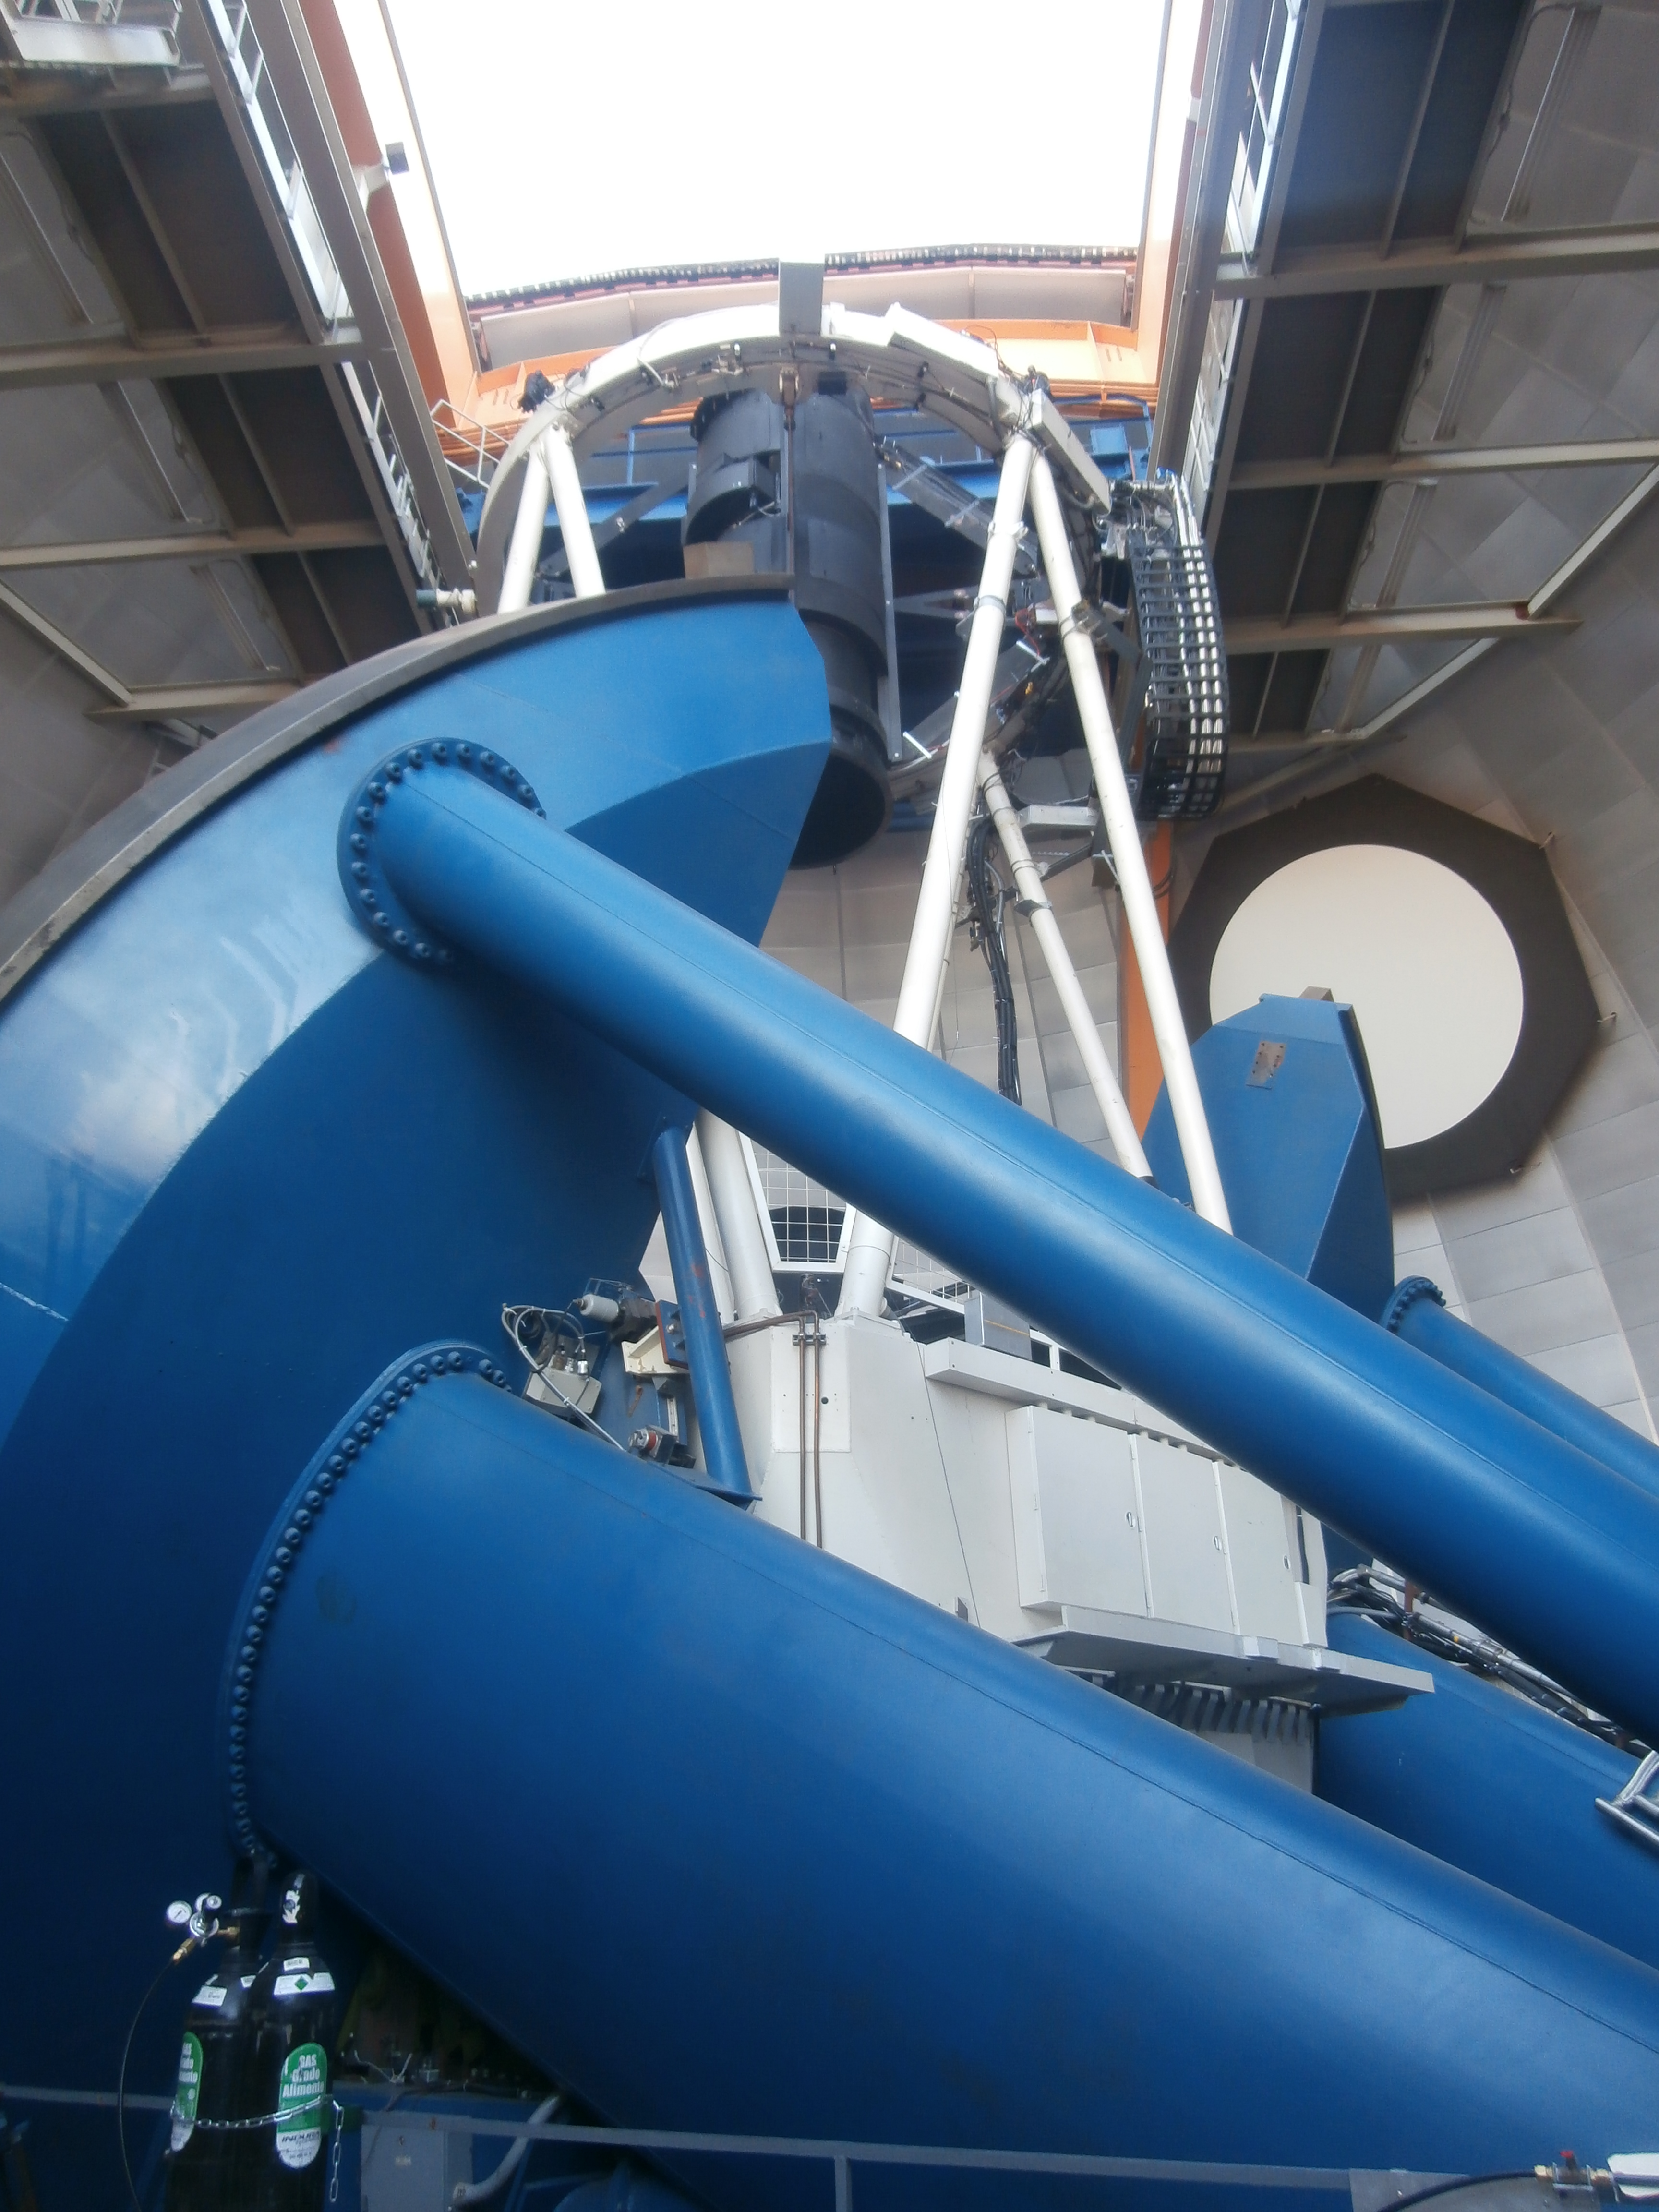
\includegraphics[width=0.9\textwidth]{./Pictures/telescope_DES_mine.jpg}
\caption{DECam mounted at the focus of the Victor Blanco Telescope. Image credit: M. Garcia-Fernandez}
\label{fig:decam}
\end{center}
\end{figure}

\section{Survey strategy}
The total amount of time awarded to DES at CTIO for observing the total area to the nominal depth on the five photometric bands is of 525 nights over a 5-year period. The rest of the nights, DECam is available to the scientific community. The tank-shaped footprint, that can be seen at \autoref{fig:des_footprint} is not casual but is optimized for the several probes.
\begin{itemize}
	\item The {\it canyon} located at the equator, is known as stripe-82 and overlaps with several spectroscopic surveys such as SDSS, to calibrate the photometric redshifts (photo-z hereafter).
    \item The rounded shape --{\it the body}-- is intended to have the largest possible scales for BAO measurement.
    \item The lower part --{\it the wheels}-- is designed to overlap with the South Pole Telescope (SPT) to measure the Sunyaev-Zel'dovich effect correlations with CMB.
\end{itemize}

\begin{figure}
\begin{center}
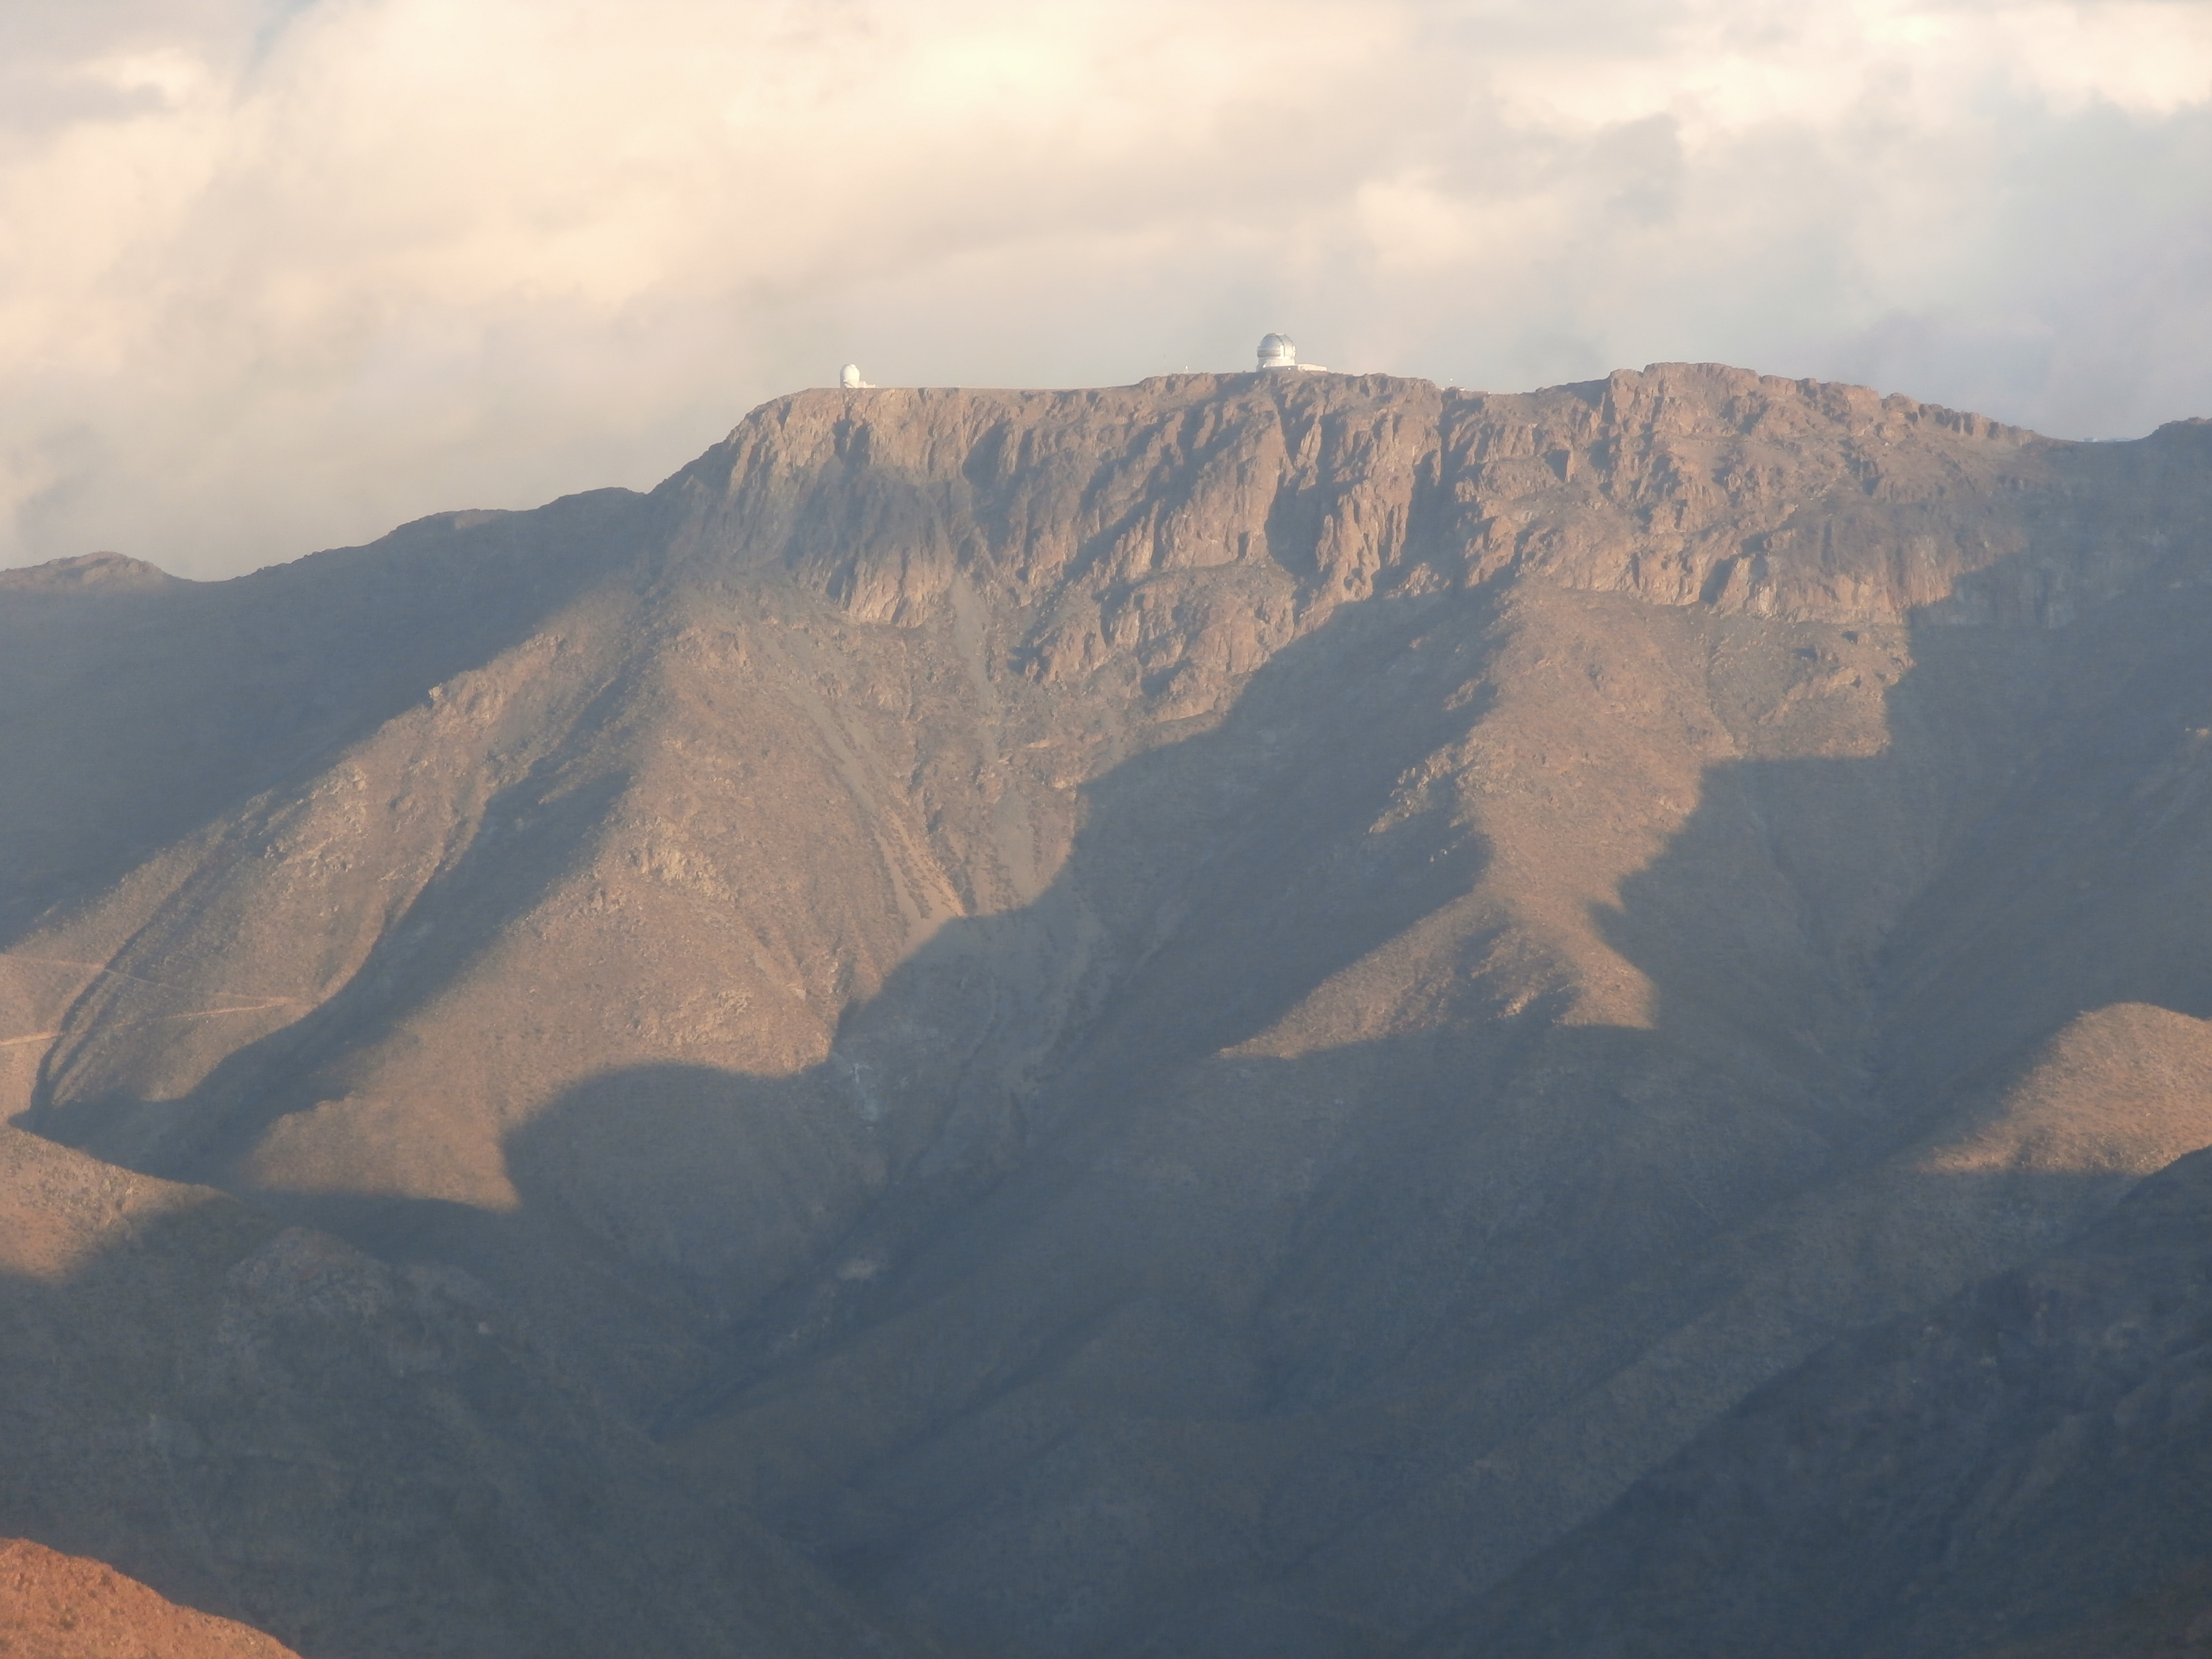
\includegraphics[width=\textwidth]{./Pictures/cerrotololo_mine.jpg}
\caption{Location of the 4-m Victor Blanco Telescope at Cerro Tololo. Chilean Andes. Image credit: M. Garcia-Fernandez}
\label{fig:cerrotololo}
\vspace{2cm}
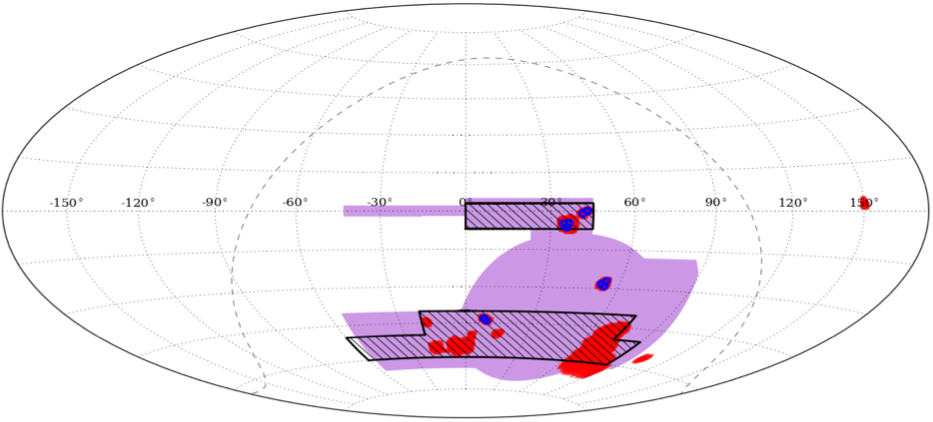
\includegraphics[width=\textwidth]{des_footprint.png}
\caption{DES footprint on equatorial coordinates. Purple area is the total area that DES will cover at the end of the five years (Y5). Red areas -that overlap with the purple- are the Science Verification observations. Shaded areas are the first year campaign of observations (Y1). Dark blue regions are the SNIa fields. Dotted line represent the galactic plane. Image credit: The DES Collaboration.}
\label{fig:des_footprint}
\end{center}
\end{figure}

The DES observations can be split in two: the transient survey and the wide-field survey.

\subsection*{The transient survey}
The transient survey is designed to measure SNIa. Selected small portions of the sky --known as the supernovae fields-- are surveyed from time to time to look for supernovae explosions and measure its luminosity curve as a function of time. Although it is designed to SNIa astronomy, some ancillary Solar-System astronomical results has been reported, such as Jupiter-trojan and trans-neptunian detection and searches for the known planet-9. These ancillary physics also use the wide-field to increase the area.

\subsection*{The wide-field survey}
The wide field survey is intended for the rest of the probes for Dark Energy. The observed area is visited 10 times on each band along the 5-year-period to reach the full depth and the maximum level of homogeneity.
\subsection*{The night operations at CTIO}
A typical night of observations, if sky is not overcast and no earthquake threatens the life of the observers, starts in the afternoon taking calibration data on CCDs. Then, after the evening twilight, three standard stars are photographed to calibrate the photometry. These, are well known stars with very well defined and measured photometric properties. After that, the wide-field survey starts. When the supernovae fields are visible --and time requirements are fulfilled--, they are surveyed, returning to the wide-field survey when they are done. Some time before the morning twilight, other three standard stars are photographed, finishing the night. All the night operations are the same except if some transient alarm us received. In this case,  DES points to the place where the transient has been produced to look for an optical counterpart.

\section{The data reduction pipeline}
The data reduction that goes from images to science-ready catalogs of galaxies is carried at the NCSA\footnote{National Center for Supercomputing Applications. Illinois (USA).}. The first step is to calibrate the data. Then, the different exposures of the same region of the sky for a given band --single-epoch images-- are combined into a single image on a procedure called co-addition --multi-epoch image--. This procedure allows the increase of the observed depth respect to each individual single-epoch image (\autoref{fig:coadd}). Nevertheless, to reach the DES nominal depth, images are detected on the $r+i+z$ multi-epoch images. This multi-epoch images will constitute the measurement images for each band. Co-addition of the objects is made with the software {\scshape Swarp} and the detection and photometric measurements is made with {\scshape SExtractor} in dual mode. {\scshape IM3SHAPE} and {\scshape NGMIX} packages are used for specific needs like shapes for shear and precise photometry.
\begin{figure}
\begin{center}
\begin{overpic}[width=0.4\textwidth,trim=0 2cm 0 0,clip]{./Pictures/destile_g.png}\put(5,5){\colorbox{white}{\Large\it g}}
\end{overpic}\hspace*{0.1cm}
\begin{overpic}[width=0.4\textwidth,trim=0 2cm 0 0,clip]{./Pictures/destile_r.png}\put(5,5){\colorbox{white}{\Large\it r}}
\end{overpic}\\
\vspace*{0.2cm}
\begin{overpic}[width=0.4\textwidth,trim=0 2cm 0 0,clip]{./Pictures/destile_i.png}\put(5,5){\colorbox{white}{\Large\it i}}
\end{overpic}\hspace*{0.1cm}
\begin{overpic}[width=0.4\textwidth,trim=0 2cm 0 0,clip]{./Pictures/destile_z.png}\put(5,5){\colorbox{white}{\Large\it z}}
\end{overpic}\\
\vspace*{0.2cm}
\begin{overpic}[width=0.4\textwidth,trim=0 2cm 0 0,clip]{./Pictures/destile_det.png}\put(5,5){\colorbox{white}{\Large coadd}}
\end{overpic}
\caption{Comparison of the multi-epoch image for the {\it griz} bands with the detection coadd. Images are taken from DES-database for a region of the tile DES0419-4914 after the Y1 epoch. Image credit: M. Garcia-Fernandez \& The DES Collaboration.}
\label{fig:coadd}
\end{center}
\end{figure}

\section{Current status and latest results}
The Dark Energy Survey began its journey on 2005 with the construction of DECam, starting the data acquisition on 2013 with the Science Verification period. By the end of February 2017, the Year 4 observation campaign has ended (\autoref{fig:des_coverage}). The Year 3 reduction pipeline from images to galaxy-catalogs has just finished and is still under inspection, so the most recent data-set that is being used for Cosmology analysis, is the Year 1 release (\autoref{fig:des_y1_coverage} and \autoref{fig:des_y1_mag_auto_i}).
\newline

Currently, no precise constrains on dark energy have been made yet, since they require an extensive and demanding control of systematic errors that is still ongoing. Nevertheless several other works on Cosmology have been provided, such as strong-lensing \cite{2015MNRAS.454.1260A,2016ApJ...827...51N,2017ApJ...838L..15L}, Sunyaev-Zel'dovich \cite{2016arXiv160508770S}, voids and troughs \cite{2016MNRAS.455.3367G,2017MNRAS.465..746S}, tests of log-normality \cite{2017MNRAS.466.1444C}, clusters \cite{2017MNRAS.467.4015H}, weak-lensing \cite{2015PhRvD..92b2006V,2016PhRvD..94b2002B,2016MNRAS.459...21K,2016MNRAS.461.3172S,2016MNRAS.461.4099B,2016arXiv160908167P,2017MNRAS.465.4204C} and large-scale-structure correlations with CMB \cite{2016MNRAS.456.3213G,2016MNRAS.459...21K,2017MNRAS.465.4166K}.
\newline

Constrains on the cosmological parameter space  provided by DES are based on the Science Verification shear analysis \cite{2016PhRvD..94b2001A,2016MNRAS.463.3653K}. Nevertheless, the most powerful measurement is produced by the combination of clustering with gg-lensing \cite{2017MNRAS.464.4045K} on the $\sigma_8-\Omega_M$ plane. Although results provided are not yet competitive, it is a remarkable milestone for DES to provide such results with just the 3\% of the planed total area (\autoref{fig:des_lcdm}).
\begin{figure}
\begin{center}
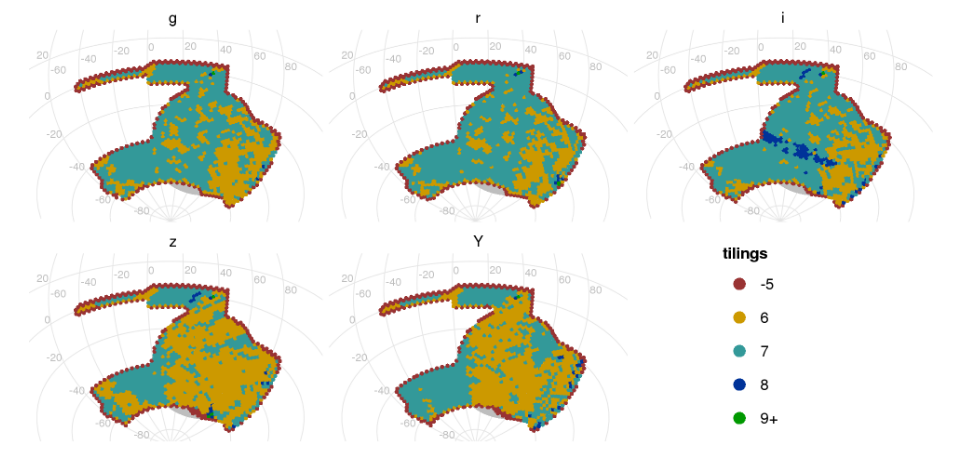
\includegraphics[width=\textwidth]{./Pictures/des_tiles.png}
\caption{DES coverage at the end of Year 4 observations campaign for the {\it grizY} photometric bands. All the area has at least 6 tiles out of 10. It can be also seen that there is plenty of area with 7 tiles. Image credit: The DES Collaboration.}
\label{fig:des_coverage}
\end{center}
\end{figure}
\begin{figure}
\begin{center}
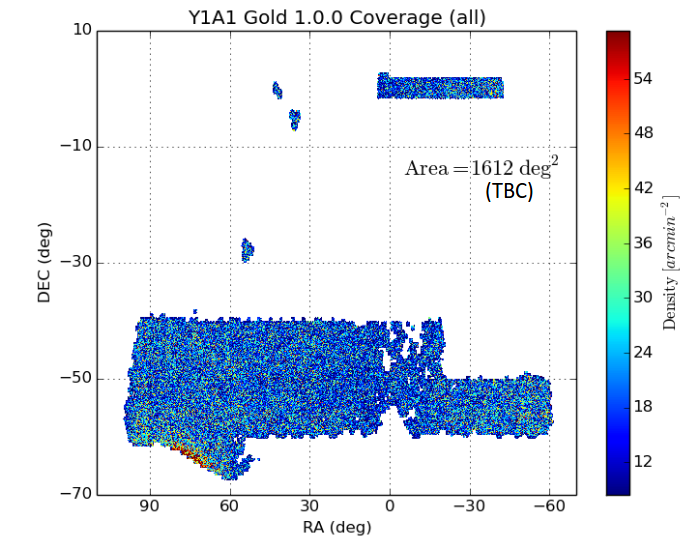
\includegraphics[width=0.9\textwidth]{./Pictures/des_y1_coverage.png}
\caption{DES Year 1 spatial distribution of objects on equatorial coordinates. Image credit: The DES Collaboration.}
\label{fig:des_y1_coverage}

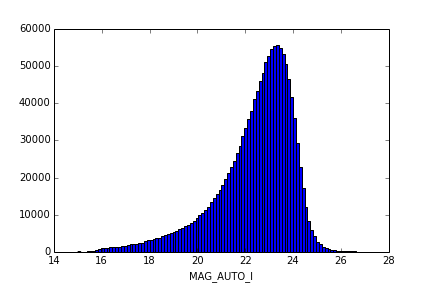
\includegraphics[width=0.9\textwidth]{./Pictures/des_y1_mag_auto_i.png}
\caption{DES Year 1 magnitude distribution of objects on the $i$-band (arbitrary normalization). The average depth reached is $i\sim 22.8$. Image credit: The DES Collaboration.}
\label{fig:des_y1_mag_auto_i}
\end{center}
\end{figure}
\newline

But not everything is about dark energy at DES. Several other results has been provided \cite{2016MNRAS.460.1270D}: discovery of several trans-neptunian objects (TNOs), Jupiter-trojans and main belt asteroids, characterization of variable stars, detection and characterization of Milky-Way satellite galaxies --and its use to put constrains on dark matter-- and gravitational-wave follow-up.

\begin{sidewaysfigure}
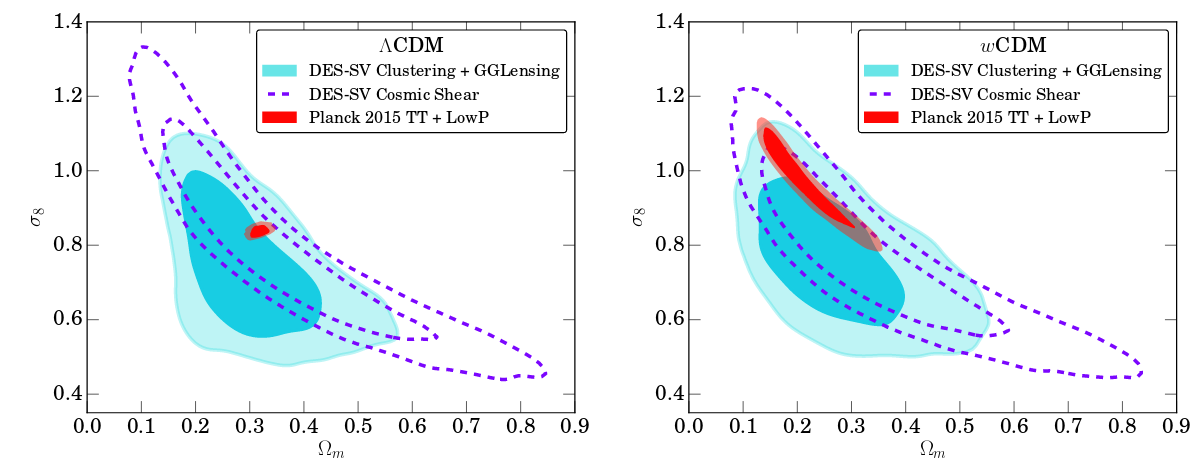
\includegraphics[width=\textwidth]{./Pictures/des_lcdm.png}
\caption{DES-SV constrains on the $\Omega_M-\sigma_8$ plane combining clustering and gg-lensing \cite{2017MNRAS.464.4045K}. Two scenarios are considered: $\Lambda$CDM and the presence of non-evolving dark energy ($w$CDM).}
\label{fig:des_lcdm}
\end{sidewaysfigure}
\chapterimage{head2.png} % Chapter heading image
\chapter{Magnification in DES}
\label{ch:magnification}

Extensive wide-field programs have allowed accurate measurements of weak-lensing effects. Previous magnification measurements involve the use of very massive objects as lenses, such as luminous red galaxies (LRGs) and clusters \cite{1995AIPC..336..320B,2014MNRAS.440.3701B,2014MNRAS.439.3755F,2016MNRAS.457.3050C}, or high redshift objects as sources, such as Lyman break galaxies (LBGs) \cite{2009A&A...507..683H,2012MNRAS.426.2489M}, quasars (QSOs) \cite{1979ApJ...227...30S,1989Natur.339..106H,1990A&A...240...11F,1993A&A...268....1B,2002A&A...386..784M,0004-637X-633-2-589} and sub-mm sources  \cite{2011MNRAS.414..596W} to improve signal-to-noise ratio. In addition to the number count technique used on this Thesis, other observational effects produced by magnification have been measured as well: the shift in magnitude \cite{2010MNRAS.405.1025M}, flux \cite{2011MNRAS.411.2113J} and size \cite{2041-8205-780-2-L16}.
\newline

On this chapter, first, the methodology to measure magnification is described (\autoref{sec:method}) and validated with simulations (\autoref{sec:mice}). Then, the methodology is used to measure the magnification signal at the Dark Energy Survey Science Verification data (SV; \autoref{sec:svdata}). Finally, the same technique used at the DES-SV data is employed to measure the convergence profile of voids and troughs with the Year 1 data (Y1; \autoref{sec:y1data}).
\newline

It is worth to remark that, as it has been defined at \autoref{ch:theory}, given both the redshift of the lenses and the sources, the convergence is a two-dimensional scalar field that is independent on the selected lens or source sample. Nevertheless, by choosing the suitable lens sample, different parts of the log-normal distribution of the convergence field \cite{2017MNRAS.466.1444C} can be probed, leading to a different convergence profile.

\section{Measuring Magnification through Number Count}
\label{sec:method}
As it has been described at \autoref{ch:theory}, the amplitude of the magnification signal is dependent on two factors: the number-count slope parameter ($\alpha-1$) and the lensing kernel, that for a given lens sample, depends on the redshift of the source sample. LBGs and QSOs has been traditionally used on magnification studies as sources since they have an steep magnitude distribution, leading to a high value of $\alpha-1$. In addition, this population of galaxies is located at very high redshift ($2\lesssim z\lesssim 4$), leading to a high lensing efficiency and a clean redshift separation between the lens and source sample. Nevertheless, this population of galaxies has much less density than the general population of galaxies, feature that can prevent the measurement of a magnification signal for low-area surveys. In addition, the selection of a population of LBGs involve the known as {\it dropout} technique, that requires the development of a custom data-reduction pipeline just to select this specific population of galaxies. For large-area surveys such as DES and LSST, the amount of computing time to run the data-reduction pipeline is enormous ($\sim 1$ year), reaching manpower and infrastructure limitations.
\newline

The caveats related to the use of LBGs and QSOs as sources can be avoided by selecting galaxies from the general population of galaxies, that is, not selecting an specific subset of the full sample of galaxies. Then, only redshift cuts are imposed in order to separate the lens and source samples. This approach has the advantage that the density of the source sample is more populated, reducing significantly the shot-noise. Nevertheless, the accuracy on the determination of the redshift on broad-band galaxy-surveys --such as DES-- is very limited, introducing an important source of systematic errors that must be avoided and carefully taken into account.
\newline

In addition to the lens-source redshift overlap, magnification suffers from several systematic errors based on the photometry \cite{2015MNRAS.454.3121M,2016MNRAS.455.3943H}, such as: depth-inhomogeneities, patchiness of the zero-point correction and calibration, or shifts on the magnitude determination due to wrong sky-background subtraction. The important reduction of shot-noise on wide-field surveys requires the development of new techniques to estimate these systematic errors.
\newline

The use of the general population of galaxies on shallow small-area surveys is mandatory to reach a significance that allows the detection of the magnification signal. On wide-area surveys the use of this population is not necessary although new studies can be made if it is used. Having a very dense population of galaxies as sources allows to use a set of lenses that are less numerous: voids and troughs. This allows to produce new physics analysis.
\newline

The usual approach that can be found on the literature to measure magnification the {\it optimal weighting} technique \cite{2003A&A...403..817M}. This methodology can be summarized as follows:
\begin{enumerate}
\item Split data sample into two well-separated photo-z bins, termed lens and source. Splitting must be done minimizing the overlap between the true redshift distributions of the samples. Otherwise, by \autoref{eq:4t}, an additive signal is introduced.
\item Weight each source galaxy by its {\it optimal weight}.
\item Compute the two-point angular cross-correlation between the lens and the unique source sample.
\end{enumerate}
The weight of the $i$-th galaxy ($w_i$) is given by:
\begin{equation}
w_i = \alpha_S(m_i)-1,
\end{equation}
where $\alpha_S(m_i)$ is the number-count slope given by \autoref{eq:alpha} and $m_i$ is the magnitude of the $i$-th galaxy. This procedure allows to obtain the maximum signal-to-noise. Nevertheless, this weighting makes hard to model the impact of the different systematic effects on the measured signal.
\newline

As an alternative approach the following procedure is proposed:
\begin{enumerate}
	\item Split the data sample into two well-separated photo-z bins, termed lens and source. Splitting must be done minimizing the overlap between the true redshift distributions of the samples. Otherwise, by \autoref{eq:4t}, an additive signal is introduced.
	\item For each photometric band, define several subsamples from the source sample using different values for the maximum (threshold) magnitude. This is made in order to trace the evolution of the amplitude of the magnification signal with the number count slope (see \autoref{eq:alpha}).
	\item Compute the two-point angular cross-correlation function between the unique common lens sample and each source subsample for each band.
\end{enumerate}
Once the two-point angular correlation function has been measured, it can be compared with theoretical predictions as described in \autoref{ch:theory} allowing the desired parameter constraints.
\newline

As has been stated previously, the amplitude of the measured cross-correlation function depends on the shape of the galaxy number count distribution. Nevertheless, due to this shape --for a fixed footprint, population of galaxies and redshift distribution--, the brighter is the magnitude limit of the sample, the bigger is the amplitude of the two point angular cross correlation function. However, the number of bright galaxies is lower than the number of faint galaxies \cite{1976ApJ...203..297S}, so shot noise is bigger at brighter magnitude cuts, increasing their measurement uncertainties. For this reason, there exists a magnitude cut that is a trade-off between amplitude and shot noise, maximizing the signal-to-noise ratio.  In  order to find the optimum magnitude cut for a given sample, define the signal-to-noise ratio for a given angular range  and magnitude cut $m'<m$ as \cite{1998MNRAS.294L..18M}:
\begin{equation}
\frac{S}{N}(m) = \frac{\langle \omega_{LS}(\theta;m)\rangle}{\langle s(\omega_{LS}(\theta;m))\rangle},
\label{eq:sn}
\end{equation}
where $\langle s(\omega_{LS}(\theta;m))\rangle$ is the average shot noise of the two point angular cross correlation functions and the averages are extended to the angular range considered in the analysis. The shot noise for a given angular aperture is given by the number of pairs inside each angular bin as
\begin{equation}
\sigma(\omega_{LS}(\theta;m)) = \frac{1}{\sqrt{P_{LS}(\theta;m)}},
\end{equation}
where $P_{LS}(\theta;m)$ is the number of pairs from the lens-source samples separated by an angular distance $\theta$ for a magnitude cut $m '<m$. The number of pairs per angular bin is given by the product of the number of source galaxies that fall inside a given annulus times the number of sources inside that annulus. Considering, as a first order approach, that the samples are uniform, the number of lens-source pair-counts of galaxies for a bin centerd at $\theta$ with solid angle $\Delta_\Omega$ is given by
\begin{equation}
P_{LS}(\theta;m) = \left[\frac{N_L}{A}\Delta_\Omega(\theta)\right]\left[\frac{N_S(m)}{A}\Delta_\Omega(\theta)\right].
\label{eq:PLS}
\end{equation}
Here $A$ is the solid angle subtended by the dataset, $N_L$ is the number of objects at the lens sample and $N_S(m)$ the number of objects on the source sample with magnitude limit $m$. Combining Equations \ref{eq:numbercountstheo}, \ref{eq:sn} and \ref{eq:PLS}, results finally in
\begin{equation}
\frac{S}{N}(m) = \langle\omega_0\rangle[\alpha(m)-1]b_L\frac{\Omega}{A}\sqrt{N_LN_S(m)},
\label{eq:snfinal}
\end{equation}
where $\Omega$ is the solid angle subtended by an annulus with edges the maximum and minimum scales considered. Thus, for a sample, given size, magnitude and redshift distributions --assuming a cosmology-- the signal-to-noise ratio can be estimated. Nevertheless, \autoref{eq:snfinal} assumes that the angular bins are uncorrelated and should be taken as an upper bound to the signal-to-noise. Although this expression does not take into account the full covariance, the behavior
\begin{equation}
\frac{S}{N} \sim [\alpha(m)-1]\sqrt{N_S(m)},
\label{eq:maxsn}
\end{equation}
is independent of cosmological and covariance assumptions up to a constant factor, allowing us to use this expression for finding the optimal cut that maximizes the signal-to-noise ratio.
\newline

\autoref{eq:maxsn} finds the magnitude cut with the maximum signal-to-noise for a given source sample. Nevertheless, this requires the use of less data than the {\it optimal weighting } approach, reaching a lower significance since less information is used. To overcome this, all the magnitude cuts within a band --not just the maximum-- are used, tracing the number-count slope evolution.

\section{Magnification in the MICE-GC simulation}
\label{sec:mice}
\begin{sidewaysfigure}
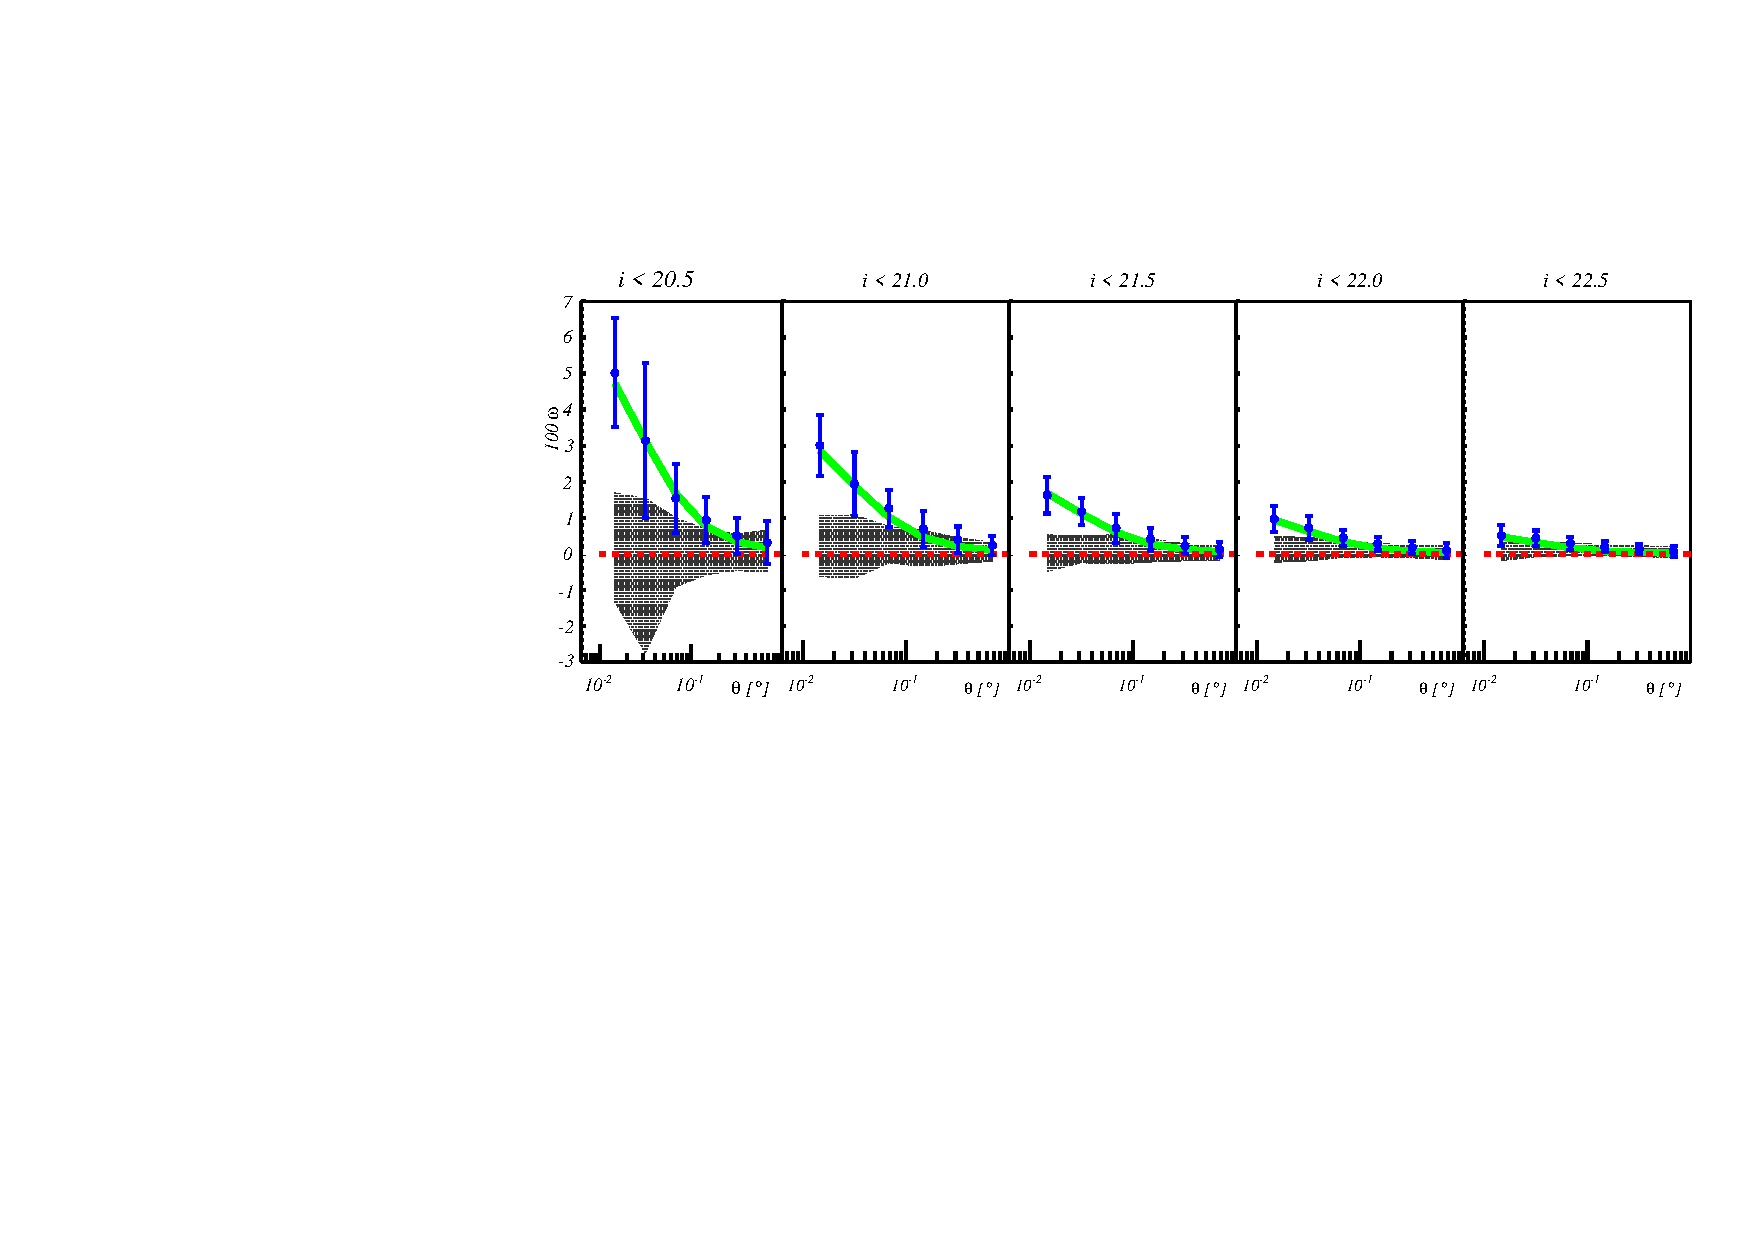
\includegraphics[width=\textwidth,trim={0 2.3cm 0 3.5cm},clip]{./figures/mag_i_MICE.pdf}
\caption{Two-point angular cross-correlation functions for the MICE simulation (sample $i < 21.5$): measured, both with magnification (blue dots) and without (grey shade), versus that expected from the MICE cosmological parameters, both with magnification (green solid line) and without (red dashed line), the latter being zero.}
\label{fig:MICE}
\end{sidewaysfigure}
In order to test the methodology described above in a controlled environment, isolated from any source of systematic error, it is applied to a simulated galaxy sample, in particular {\scshape MICECAT v1.0}.
This mock is the first catalog release of the N-body simulation MICE-GC\footnote{www.ice.cat/mice} \cite{2015MNRAS.447.1319F,2015.2987F,2015MNRAS.453.1513C}. It assumes a flat $\Lambda$CDM Universe with cosmological parameters $\Omega_M=0.25, \Omega_b=0.044, h=0.7$ and $\sigma_8 = 0.8$, using a light-cone that spans one eighth of the celestial sphere. Another advantage of using these simulations is the possibility of studying specific systematic effects, as described in \autoref{sec:sys}.

Among other properties, MICE-GC provides lensed and unlensed coordinates, true redshift (including redshift space distortions) and DES-$griz$ unlensed magnitudes for the simulated galaxies, along with convergence and shear.
Conversion from unlensed magnitudes to lensed magnitudes can be done by applying $m_\mu = m_0-2.5\log_{10}(1+2\kappa)$.

Having two sets of coordinates and magnitudes, one in a `universe' with magnification and another without magnification, allows us to follow the methodology described in \autoref{sec:method} for both cases,
serving as a test-bench to measure the sensitivity of the method to the magnification effect. In order to have a fiducial function with as little statistical uncertainty as possible, the full 5000 deg$^2$ of the MICE simulation are used. To match as much as possible the conditions of the DES-SV data, the magnitude cuts described in \autoref{sec:data_sample_SV} are applied to the lens and source samples. The covariance matrices of data (see \autoref{sec:svdata}) are used, in order to match the errors in the DES-SV sample.

In \autoref{fig:MICE}, the results of the magnification analysis in the MICE simulation for the cases with and without magnification can be seen compared with the theoretical expectations. The methodology used in this work clearly allows us to distinguish both cases for a data-set similar to that of the DES-SV data. Nevertheless, results obtained with the MICE simulation can not be directly extrapolated to SV data to estimate the expected significance because the density of galaxies on the simulation is a factor $\sim3$ smaller than on the SV data. Also, the luminosity function of the simulation is slightly different from the DES data, which has a direct impact on the number count slope and, consequently, on the amplitude of the measured signal.


\section{Magnification in DES Science Verification data}
\label{sec:svdata}
As of January 2014 --when I started my PhD--, the only data available at DES was the Science Verification data. The first data-release from DES. This data were taken just for testing purposes and in order to explore the capabilities of the experiment. Thus, although the nominal depth of the survey was reached, only $\sim 150$ deg$^2$ where taken. Taking this into account, only $10^4$ LBGs are expected at the full DES-SV data, preventing the measurement of magnification with the usual approach. Thus, in order to be capable to reach a detection of the magnification signal with the DES-SV data, the general population of galaxies was selected both as lens and source sample.
\newline

The goal of this analysis is to detect a weak-lensing magnification signal and develop methodology to mitigate systematic errors. Data sample is described at \autoref{sec:data_sample_SV}. Then, the analysis is described and the results discussed at \autoref{sec:analysis_sv} following the analysis of the possible systematic errors on \autoref{sec:sys}. Finally a discussion on the analysis can be found at \autoref{sec:discussion_sv}.

\subsection{Data sample}
\label{sec:data_sample_SV}
From the DES SVA1-Gold\footnote{des.ncsa.illinois.edu/releases/SVA1} main galaxy catalog \cite{2016MNRAS.455.4301C}, the largest contiguous field is selected, the SPT-E. Regions with declination $ < -61^{\circ}$ are removed in order to avoid the Large Magellanic Cloud. {\scshape Modest\_class} is employed as star-galaxy classifier \cite{0004-637X-801-2-73}.
\newline

The following color cuts are made in order to remove outliers in color space:
\begin{itemize}
	\item $-1 < g-r < 3$,
	\item $-1 < r-i < 2$,
	\item $-1 < i-z < 2$;
\end{itemize}
where {\it g}, {\it r}, {\it i}, {\it z} stand for the corresponding {\scshape mag\_auto} magnitude measured by {\scshape SExtractor} \cite{1996A&AS..117..393B}.
\newline

Regions of the sky that are tagged as bad, amounting to four per cent of the total area, are removed. An area of radius 2 arcminutes around each 2MASS star is masked to avoid stellar halos \cite{2005MNRAS.361.1287M,0004-637X-633-2-589}.
\newline

The DES Data Management \cite{2011arXiv1109.6741S,2012ApJ...757...83D,2012SPIE.8451E..0DM} produces a {\scshape mangle}\footnote{http://space.mit.edu/$\sim$molly/mangle/} \cite{2008MNRAS.387.1391S}  magnitude limit mask that is later translated to a $N_{\rm side}=4096$ {\scshape HEALPix}\footnote{healpix.jpl.nasa.gov} \cite{2005ApJ...622..759G} mask. Since the {\scshape HEALPix} mask is a division of the celestial sphere with romboid-like shaped pixels with the same area, to avoid boundary effects due to the possible mismatch between the {\scshape mangle} and {\scshape HEALPix} masks, each pixel is required to be totally inside the observed footprint as determined by {\scshape mangle}, by demanding
\begin{itemize}
	\item $r_{\rm fracdet}=1$,
	\item $i_{\rm fracdet}=1$,
	\item $z_{\rm fracdet}=1$;
\end{itemize}
where $r_{\rm fracdet},i_{\rm fracdet},z_{\rm fracdet}$ is the fraction of the pixel lying inside the footprint for {\it r}, {\it i}, {\it z} bands respectively.
\newline

Depth cuts are also imposed on the {\it riz}-bands in order to have uniform depth when combined with the magnitude cuts. These depth cuts are reached by including only the regions that meet the following conditions:
\begin{itemize}
	\item $r_{\rm lim} > 23.0$,
	\item $i_{\rm lim} > 22.5$,
	\item $z_{\rm lim} > 22.0$;
\end{itemize}
where $r_{\rm lim}, i_{\rm lim},z_{\rm lim}$ stand for the magnitude limit in the corresponding band, that is, the faintest magnitude at which the flux of a galaxy is detected at 10$\sigma$ significance level. The resulting footprint, as shown in \autoref{fig:footprint}, after all the masking cuts amounts to $121 \mbox{ deg}^2$.
\begin{figure}
\begin{center}
\begin{flushright}
\begin{overpic}[width=0.85\textwidth]{./figures/footprint.pdf}
\put(85,0){RA [$^\circ$]}
\put(-5,70){\rotatebox{90}{DEC [$^\circ$]}}
\end{overpic}
\end{flushright}
\caption{Final footprint of the DES SPT-E region after all masking is applied.}
\label{fig:footprint}
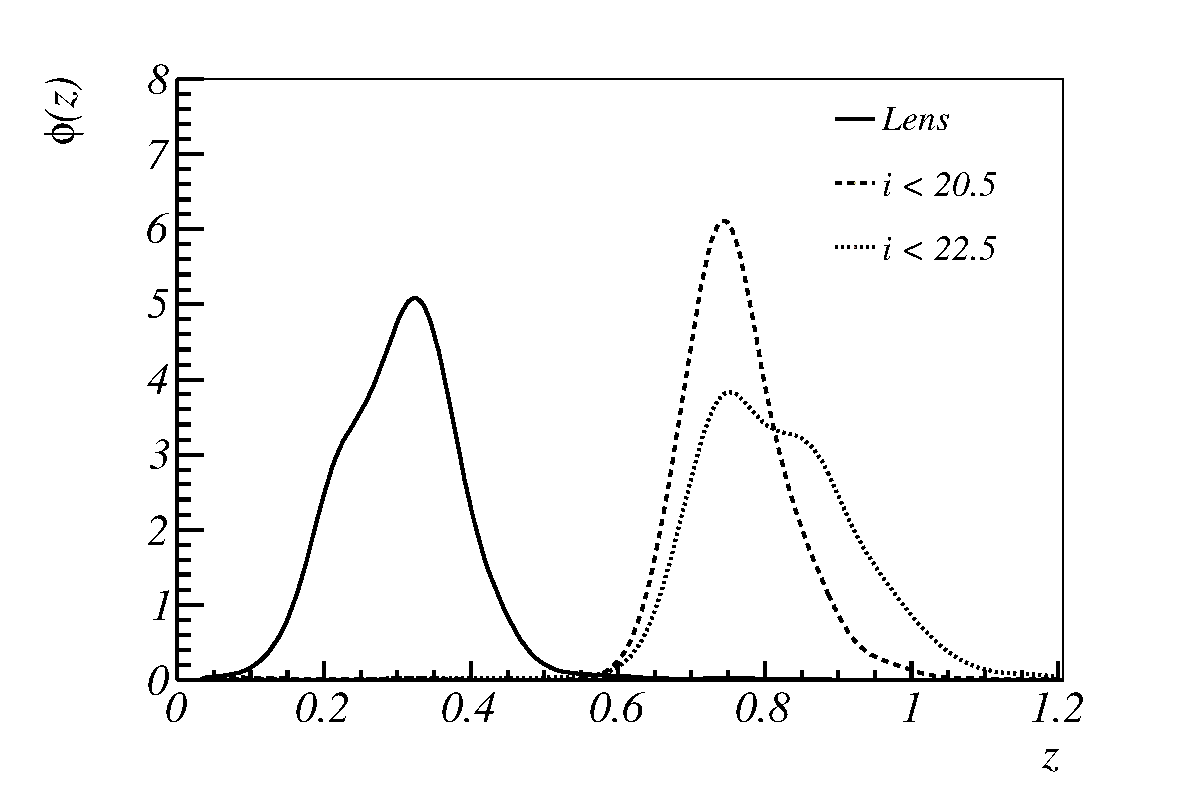
\includegraphics[width=0.85\textwidth]{./figures/TPZ_phis_i.pdf}
\caption{Redshift distributions from the stacking of the TPZ probability distribution functions for the lens and two {\it i}-band sub-samples of the source.}
\label{fig:stacking}
\end{center}
\end{figure}
\newline

Photometric redshifts (photo-z) have been estimated using different techniques. In particular, the fiducial code used in this work employs a machine-learning algorithm (random forests) as implemented by TPZ \cite{2013MNRAS.432.1483C}, which was shown to perform well on SV data \cite{2014MNRAS.445.1482S}. The redshifts of the galaxies are defined according to the mean of the probability density functions given by TPZ ($z_{\rm ph}$). Other methods are also employed to demonstrate that the measured two-point angular cross-correlation are not a feature induced by TPZ.

\subsubsection{Lens sample}
A unique lens sample is defined by the additional photo-z and magnitude cuts:
\begin{itemize}
	\item $0.2 < z_{\rm ph} < 0.4$;
	\item $18.0 < i < 22.5$.
\end{itemize}
These requirements are imposed in order to be compatible with the first redshift bin of the so called `benchmark sample' \cite{2016MNRAS.455.4301C}. Note that the {\scshape mag\_auto} cut along with the previous $i$-band depth cut guarantees uniformity \cite{2016MNRAS.455.4301C}.

\subsubsection{Source sample}
Three source samples are defined, one per band:
\begin{itemize}
	\item R: $0.7 < z_{\rm ph} < 1.0$ and $r<23.0$;
	\item I: $0.7 < z_{\rm ph} < 1.0$ and $i<22.5$;
	\item Z: $0.7 < z_{\rm ph} < 1.0$ and $z<22.0$.
\end{itemize}

Following the same approach we used on the lens, defined over the `benchmark' sample, the {\scshape mag\_auto} cut along with the previously defined depth cuts also guarantee uniformity on the corresponding band. Within each R, I, Z source sample five sub-samples that map the magnitude evolution are defined,
\begin{itemize}
	\item $\rm R_1$: $r<21.0$; $\rm R_2$: $r<21.5$; $\rm R_3$: $r<22.0$; $\rm R_4$: $r<22.5$; $\rm R_5$: $r<23.0$.
	\item $\rm I_1$: $i<20.5$; $\rm I_2$: $i<21.0$; $\rm I_3$: $i<21.5$; $\rm I_4$: $i<22.0$; $\rm I_5$: $i<22.5$.
	\item $\rm Z_1$: $z<20.0$; $\rm Z_2$: $z<20.5$; $\rm Z_3$: $z<21.0$; $\rm Z_4$: $z<21.5$; $\rm Z_5$: $z<22.0$.
\end{itemize}
Here $\rm S_j$ with $\rm j=1,2,3,4,5$ are the sub-samples of sample S with $\rm S\in \{R,I,Z\}$. In \autoref{fig:stacking}, the redshift distributions of the lens and source sample are shown. Note that the sub-samples $\rm R_5, I_5, Z_5$ are equal to $\rm R, I , Z$ respectively.
\newline

The {\it g}-band is not used on this analysis because when the same approach is followed and a uniform sample is defined in that band, the number of galaxies of the lens and source samples decrease dramatically. This increases the shot noise preventing the measurement of number count magnification

\subsection{Detection of the weak-lensing magnification signal}
\label{sec:analysis_sv}
To estimate the cross-correlation functions, the tree-code {\scshape TreeCorr}\footnote{github.com/rmjarvis/TreeCorr} \cite{2004MNRAS.352..338J} and the Landy-Szalay estimator \cite{1993ApJ...412...64L} are used demanding six logarithmic angular bins:
\begin{equation}
\omega_{\rm LS_j}(\theta) = \frac{D_{\rm L}D_{\rm S_j}(\theta)-D_{\rm L}R_{\rm S_j}(\theta)-D_{\rm S_j}R_{\rm L}(\theta)}{R_{\rm L}R_{\rm S_j}(\theta)}+1,
\label{eq:landyszalay}
\end{equation}
where $D_{\rm L}D_{\rm S_j}(\theta)$ is the number of pairs from the lens data sample L and the source data sub-sample $\rm S_j$ separated by an angular distance $\theta$ and $D_{\rm L}R_{\rm S_j}(\theta)$, $D_{\rm S_j}R_{\rm L}(\theta)$, $R_{\rm L}R_{\rm S_j}(\theta)$ are the corresponding values for the lens-random, source-random and random-random combinations normalized by the total number of objects on each sample.
\newline

Catalogs produced with {\scshape Balrog}\footnote{github.com/emhuff/Balrog} \cite{2016MNRAS.457..786S} are used as random sample. See \autoref{sec:balrog} for a detailed description and discussion on this.
\newline

A covariance matrix is computed for each band by jack-knife re-sampling the data taking into account the correlations between the different magnitude cut within each band
\begin{eqnarray}
C_{\rm S}(\omega_{\rm LS_i}(\theta_\eta);\omega_{\rm LS_j}(\theta_\nu)) = \frac{N_{\rm JK}}{N_{\rm JK}-1}\\
\times \sum\limits_k^{N_{\rm JK}}[\omega_{\rm LS_i}^k(\theta_\eta)-\omega_{\rm LS_i}(\theta_\eta)][\omega_{\rm LS_j}^k(\theta_\nu)-\omega_{\rm LS_j}(\theta_\nu)]\nonumber,
\end{eqnarray}
where $\omega^k_{\rm LS_j}$ stands for the cross-correlation of the $k$-th jack-knife re-sample and $\omega_{\rm LS_j}$ is the cross-correlation of the full sample. The $N_{\rm JK}= 120$ jack-knife regions are defined by a $k$-means algorithm \cite{macqueen1967some} using Python's machine learning library {\scshape scikit-learn}\footnote{scikit-learn.org} \cite{scikit-learn}. In order to get $N_{\rm JK}$ regions with equal area, the algorithm is trained on a uniform random sample following the footprint of the data demanding $N_{\rm JK}$ centers. The regions used on the re-sampling are composed by the Voronoi tessellation defined by these centers. These matrices trace the angular covariance as well as the covariances between functions within each band. No covariance between bands is considered, since each band is treated independently on this work. The reduced covariance matrix of the {\itshape i}-band is displayed at \autoref{fig:cov_matrix}. The behaviour is similar for the other bands.
\begin{figure}
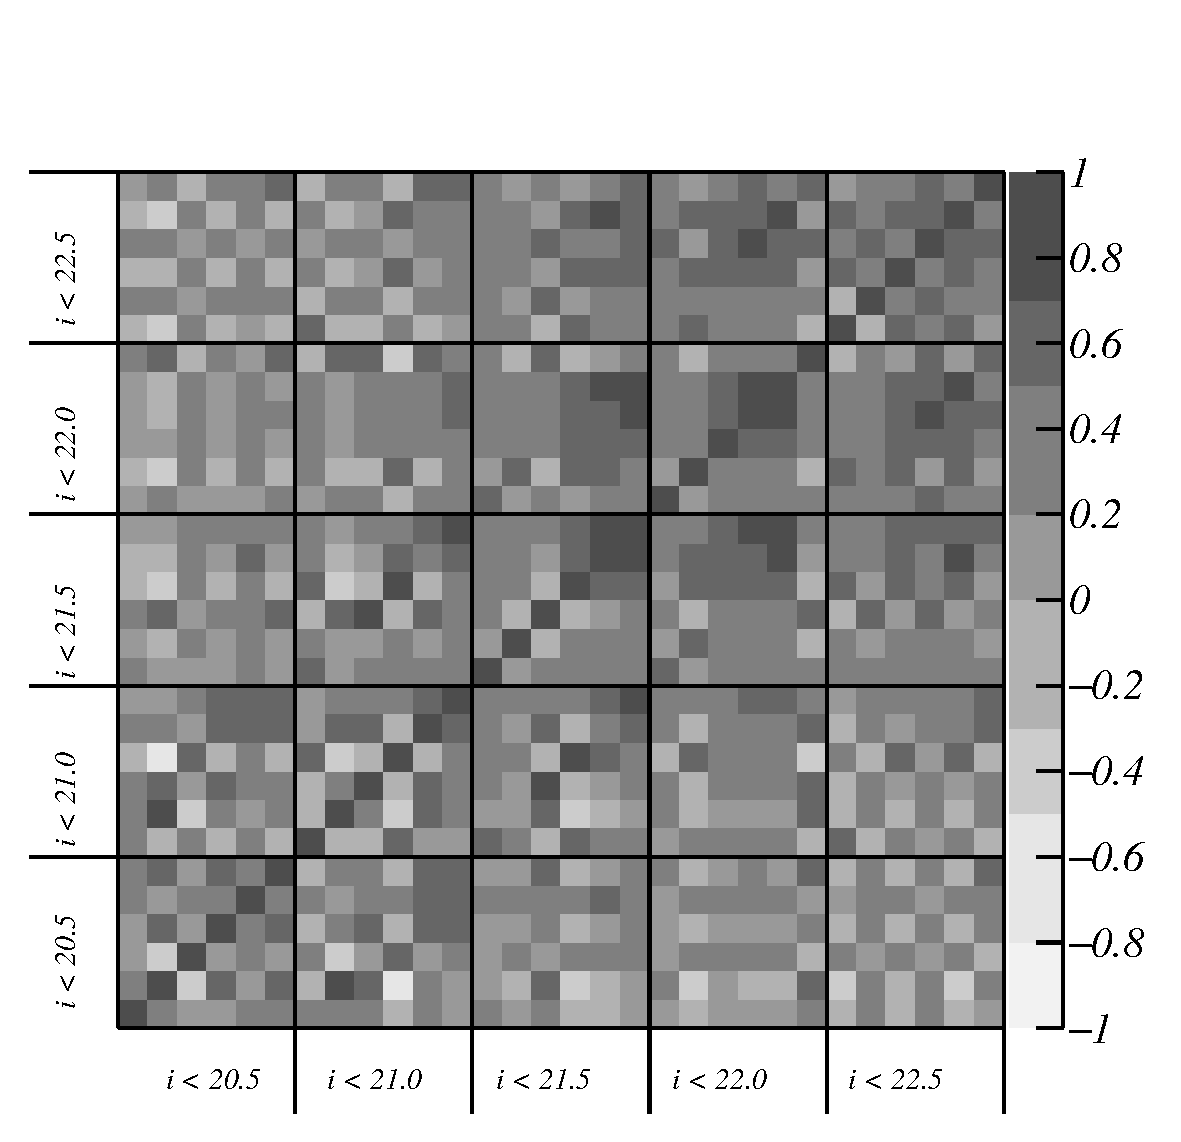
\includegraphics[width=\textwidth,trim={0 0 0 2cm},clip]{./figures/cov_matrix_mag_auto_i.pdf}
\caption{Covariance matrix of the {\it i}-band rescaled by the value of the diagonal ($C_{ij}/\sqrt{C_{ii}C_{jj}}$). Each box is the part of the matrix corresponding to the samples labeled at the axis whereas the bins within each box stand for the angular values of the correlation function.}
\label{fig:cov_matrix}
\end{figure}
\newline

Measured two-point angular cross-correlation functions and $\Lambda$CDM weak lensing theoretical predictions can be found in \autoref{fig:resultsSV_r}, \autoref{fig:resultsSV_i} and \autoref{fig:resultsSV_z}. Measured correlation functions are found to be non-zero, compatible with $\Lambda$CDM and its amplitude evolves with the magnitude cut. The magnitude cuts imposed to guarantee uniform depth make that, for this data, no negative amplitudes are expected.
\begin{sidewaysfigure}
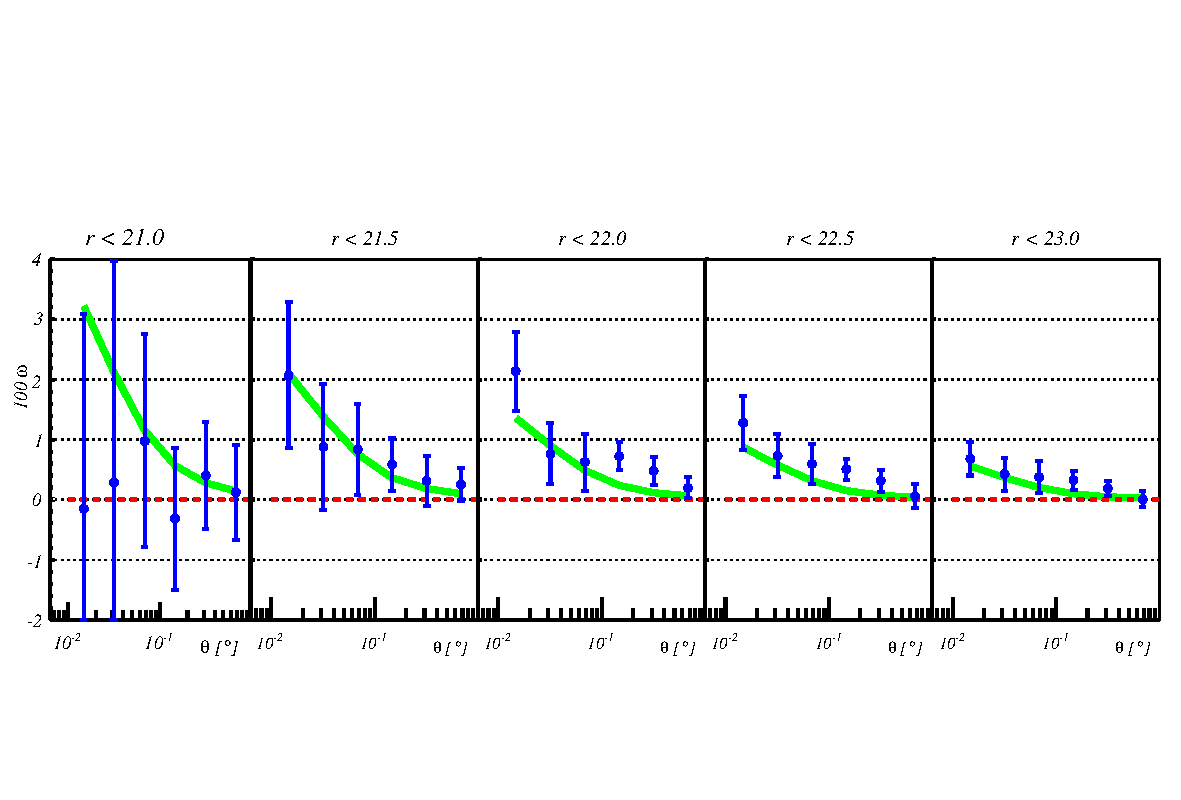
\includegraphics[width=\textwidth,trim={0 2.3cm 0 3.5cm},clip]{./figures/mag_r.pdf}
\label{fig:resultsSV_r}
\caption{Magnification signal for the DES-SV {\it r}-band sample.}
\end{sidewaysfigure}
\begin{sidewaysfigure}
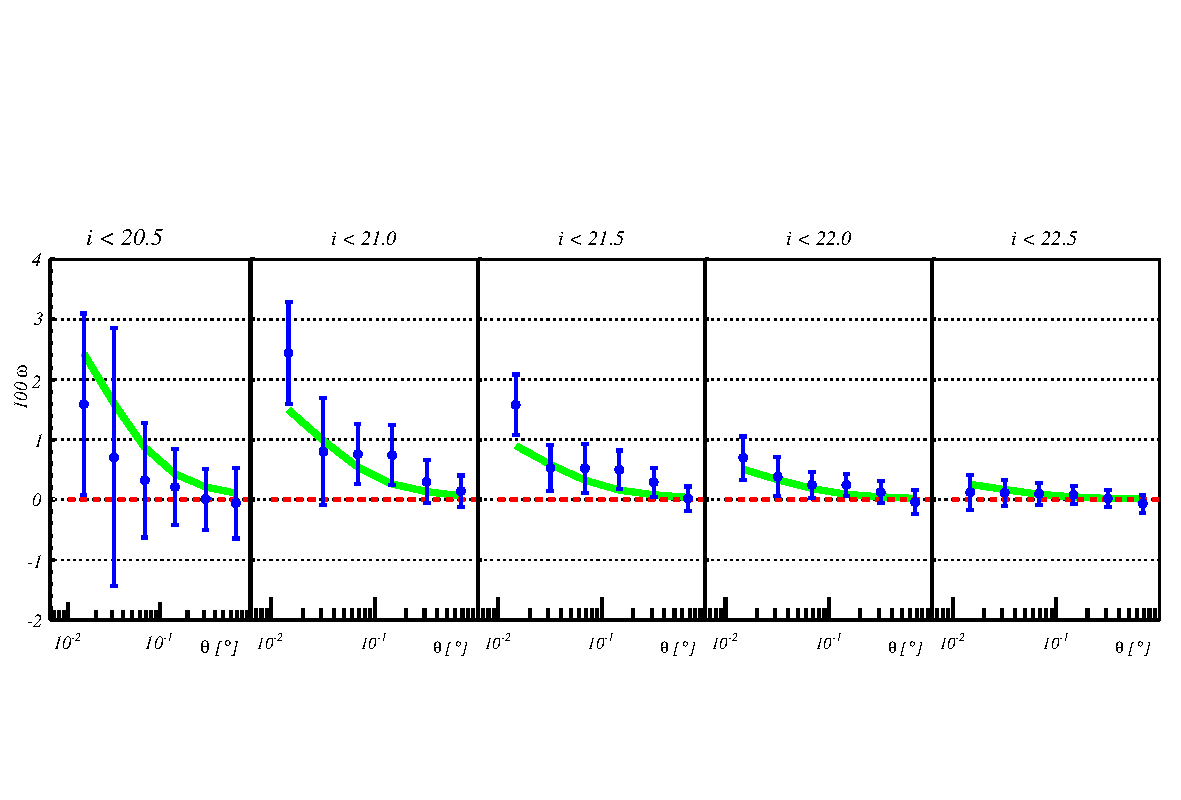
\includegraphics[width=\textwidth,trim={0 2.3cm 0 3.5cm},clip]{./figures/mag_i.pdf}
\label{fig:resultsSV_i}
\caption{Magnification signal for the DES-SV {\it i}-band sample.}
\end{sidewaysfigure}
\begin{sidewaysfigure}
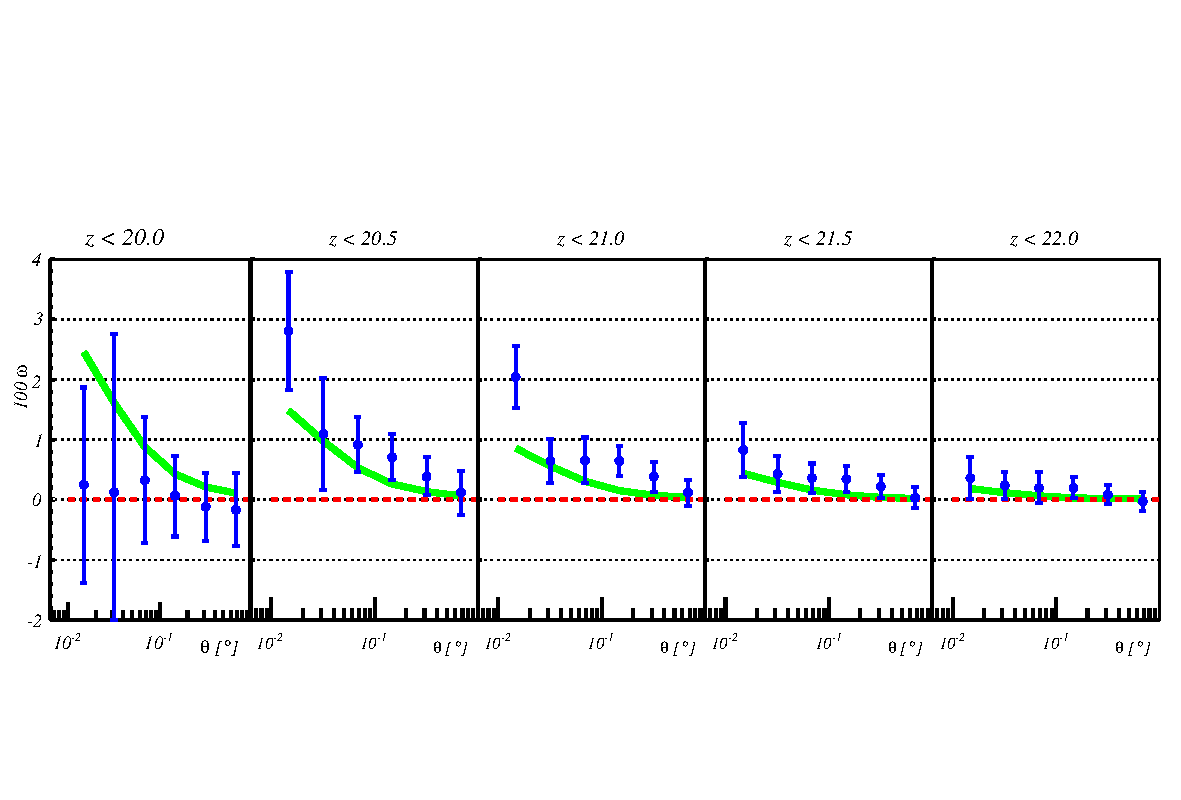
\includegraphics[width=\textwidth,trim={0 2.3cm 0 3.5cm},clip]{./figures/mag_z.pdf}
\label{fig:resultsSV_z}
\caption{Magnification signal for the DES-SV {\it z}-band sample.	}
\end{sidewaysfigure}
\newline

To compare with the expected theory, \autoref{eq:kappa_nc} and \autoref{eq:omega0} and  have been used assuming Planck 2015 \cite{2016A&A...594A..13P} cosmological parameters. The bias of the lens sample has already been measured independently with different techniques: clustering \cite{2016MNRAS.455.4301C}, gg-lensing \cite{2016arXiv160908167P}, shear \cite{2016MNRAS.459.3203C} and CMB-lensing \cite{2016MNRAS.456.3213G}. From these values the most precise, from \cite{2016MNRAS.455.4301C}, is selected ($b_{\rm L}=1.07\pm0.08$) and is assumed to be a constant scale-independent parameter. The number count slope parameter $\alpha_{\rm S}$ is computed by fitting the cumulative number count of the sample S to a Schechter function \cite{1976ApJ...203..297S} on the range of interest
\begin{equation}
N_\mu(m) = A\left[10^{0.4(m-m_*)}\right]^\beta\times\exp\left[-10^{0.4(m-m*)}\right],
\label{eq:sch}
\end{equation}
where $A,m_*,\beta$ are the free parameters of the fit. Then $\alpha_{\rm S}(m)-1$ is computed by applying \autoref{eq:alpha}, where $m_{\rm j}$ is the magnitude limit of the $\rm S_j$ sub-sample on the considered band. In \autoref{fig:alphai} the fit and the number count slope parameter for the I sample are shown.
\begin{figure}
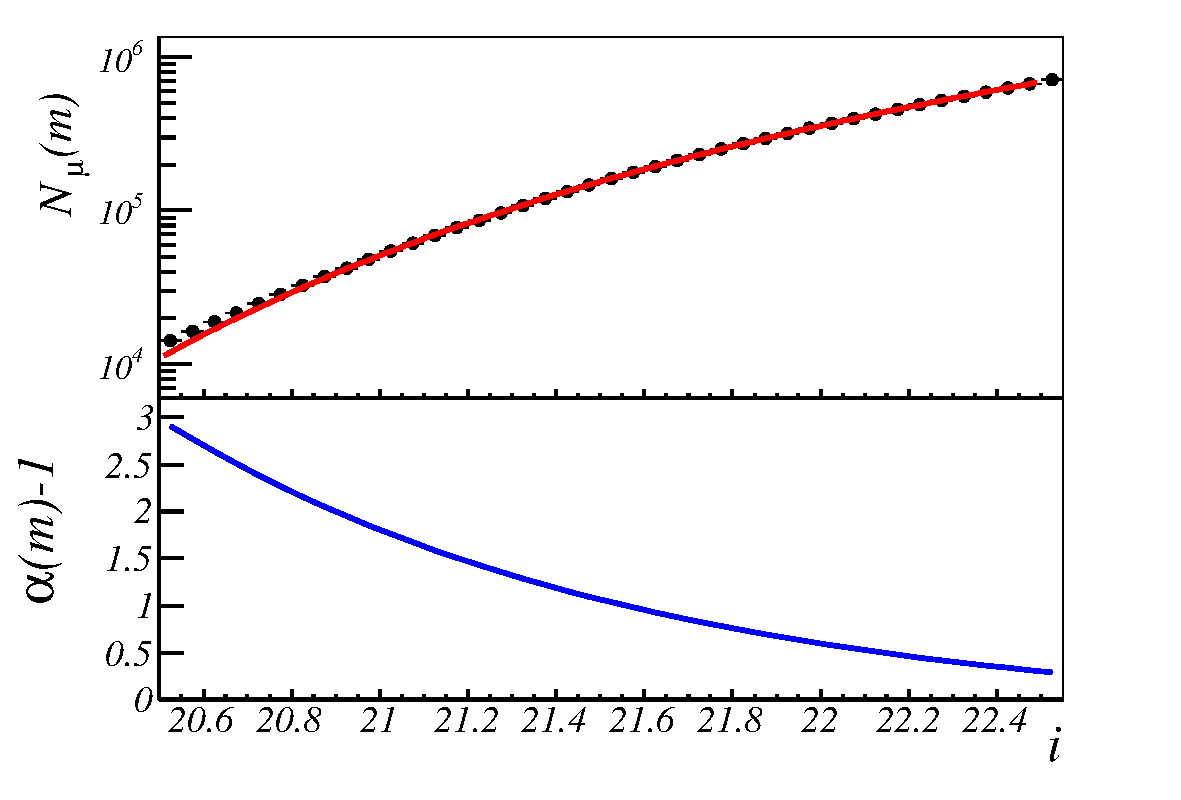
\includegraphics[width=0.85\textwidth]{./figures/alphai.pdf}
\caption{Top panel: Dots are the measured {\it i}-band cumulative number count as a function of the {\it i}-band magnitude. Red solid line is the fit using a Schechter function (see text). Bottom panel: number count slope $\alpha-1$ measured from the fitted Schechter function of the top panel.}
\label{fig:alphai}
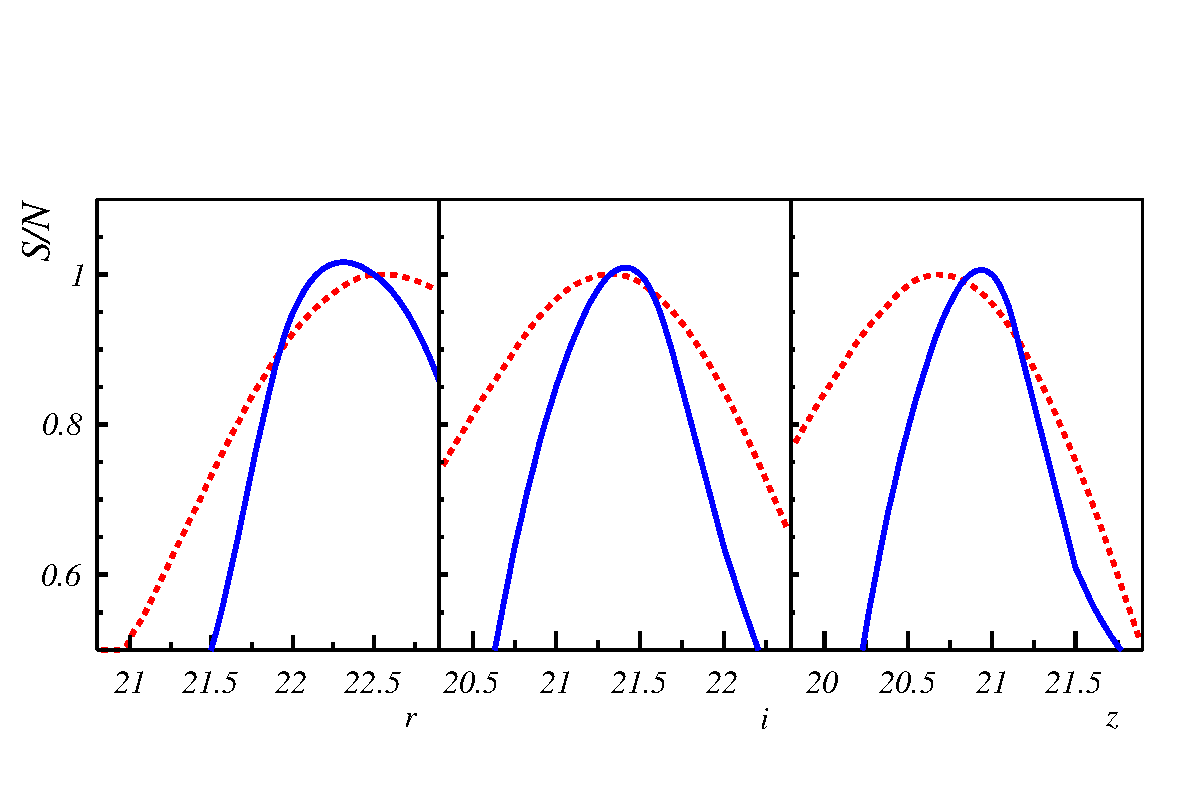
\includegraphics[width=0.85\textwidth,trim={0 1.0cm 0 2.5cm},clip]{./figures/predicted_sig.pdf}
\caption{Red dashed line: expected signal-to-noise ratio computed with \autoref{eq:sn}. Blue solid line is the measured significance of the data. Both curves are normalized to their respective maximum.}
\label{fig:significance}
\end{figure}
\begin{table}
\begin{center}\begin{tabular}{ c | c | c c }
 Weight& Sample & $\log_{10}\mathcal{B}$ & $\chi^2/ndof$  \\
\hline
 & R & 3.9 & 21.6/30\\
 No& I & 3.4 & 23.9/30\\
 & Z & 3.4 & 36.8/30\\
\hline
 & $r<23.0$ & 3.2 & 3.2/6\\
 Yes& $i < 22.5$ & 2.1&2.1/6\\
 & $z<22.0$ & 2.3&2.3/6\\
\end{tabular}\end{center}
\caption{Significance of the detection of a magnification signal. Results are shown for the combination of the five subsamples within each band as well as for the faintest sample with weighting.}
\label{tab:significance}
\end{table}
\newline

A goodness of fit test of the measured two-point angular cross-correlation function respect to the theoretical predictions for each band is performed:
\begin{eqnarray}
&\chi^2_{\rm Planck} =\sum\limits_{\eta\nu ij}[\tilde \omega_{\rm LS_i}(\theta_\eta)-\omega_{\rm LS_i}(\theta_\eta)]\\
&C^{-1}(\omega_{\rm LS_i}(\theta_\eta);\omega_{\rm LS_j}(\theta_\nu))[\tilde \omega_{\rm LS_j}(\theta_\nu)-\omega_{\rm LS_j}(\theta_\nu)],
\end{eqnarray}
where $\tilde\omega,\omega$ are the measured and theoretical cross-correlation functions respectively. Goodness of fit tests are also made testing the hypothesis of absence of magnification:
\begin{eqnarray}
&\chi^2_{\rm zero}=\\
&\sum\limits_{\eta\nu ij}\tilde\omega_{\rm LS_i}(\theta_\eta)C^{-1}(\omega_{\rm LS_i}(\theta_\eta);\omega_{\rm LS_j}(\theta_\nu))\tilde\omega_{\rm LS_j}(\theta_\nu)\nonumber.
\end{eqnarray}
The $\chi^2$ values can be seen in \autoref{tab:significance} showing good agreement with the theoretical predictions described in \autoref{ch:theory}. To test which hypothesis is favored, the Bayes factor is used:
\begin{equation}
\mathcal{B} = \frac{P(M|\Theta)}{P(Z|\Theta)} = \frac{P(\Theta |M)}{P(\Theta|Z)}\frac{P(M)}{P(Z)},
\end{equation}
where 
\begin{equation}
P(M|\Theta) = e^{-\chi^2_{\rm Planck}/2}
\end{equation}
and
\begin{equation}
P(Z|\Theta) = e^{-\chi^2_{\rm zero}/2}.
\end{equation}
The assumed prior sets detection and non-detection of magnification to be equally probable: $P(M) = P(Z)$. Bayes factors are computed for each function individually as well as for each band using the full covariance.
\newline

The significance for each individual correlation function has a strong dependence on the considered magnitude limit of the sub-sample. At the bright cuts, shot-noise prevents the identification of a non-zero magnification signal. At the faint end, although the sub-samples are much more populated, the strength of the magnification signal is compatible with zero. This behaviour has been compared with the predictions (see \autoref{sec:method}). Predicted and measured values are plotted together in \autoref{fig:significance}. It can be seen that the prediction of the location of the maximum signal-to-noise can only be used as a first approach.
\newline

To compute the significance of the detection for each band, the full covariance is used. One covariance matrix (see \autoref{fig:cov_matrix} for the {\itshape i}-band matrix) per each band is computed taking into account the correlations between each magnitude cut. The logarithm of the Bayes factor can be found in \autoref{tab:significance}, being all above 2, allowing to claim that magnification has been detected \cite{10.2307/2291091}.
\newline
 
 A usual approach to enhance the signal-to-noise ratio, is to define a unique source sample and weight each source galaxy with its corresponding $\alpha_S(m)-1$ value \cite{2003A&A...403..817M} and compute the two-point angular cross-correlation function. This weighting procedure is used at the samples $r < 23.0$, $i < 22.5$ and $z < 22.0$. These correlation functions can be seen in \autoref{fig:reweight} with a comparison with the theoretical prediction and the correlation functions of the same sample computed without weighting. Significances of these measurement can be found in \autoref{tab:significance} with a marginal difference respect to the one computed without weighting using the five subsamples.
\begin{figure}
\begin{center}
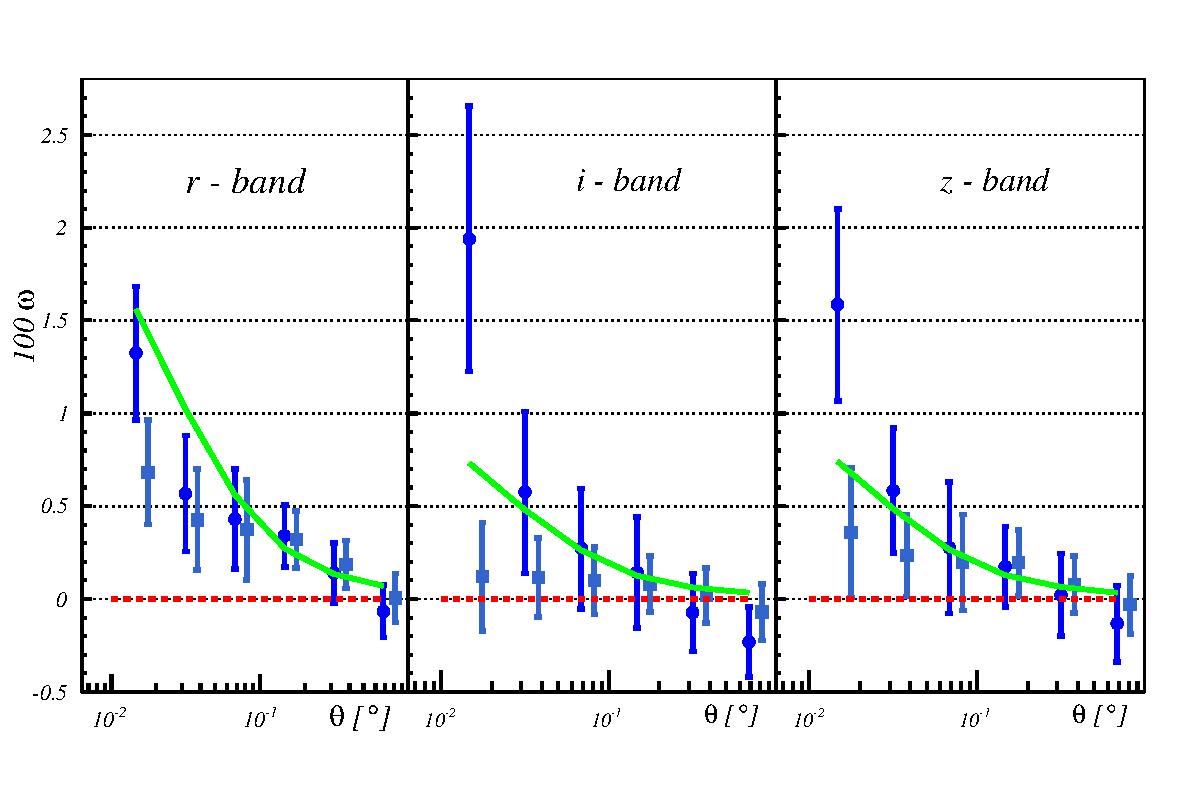
\includegraphics[width=0.85\textwidth]{./figures/weighted_w.pdf}
\caption{Measured two-point angular cross-correlation functions for the samples $r<23.0$, $i < 22.5$ and $z < 22.0$ left to right respectively. Dots use the optimal weighting \cite{0004-637X-633-2-589}, where each galaxy is weighted by its corresponding $\alpha_S(m)-1$ value, whereas squares are not weighted. Green line is the theoretical prediction. Red dashed line is an eye-guide for zero.}
\label{fig:reweight}
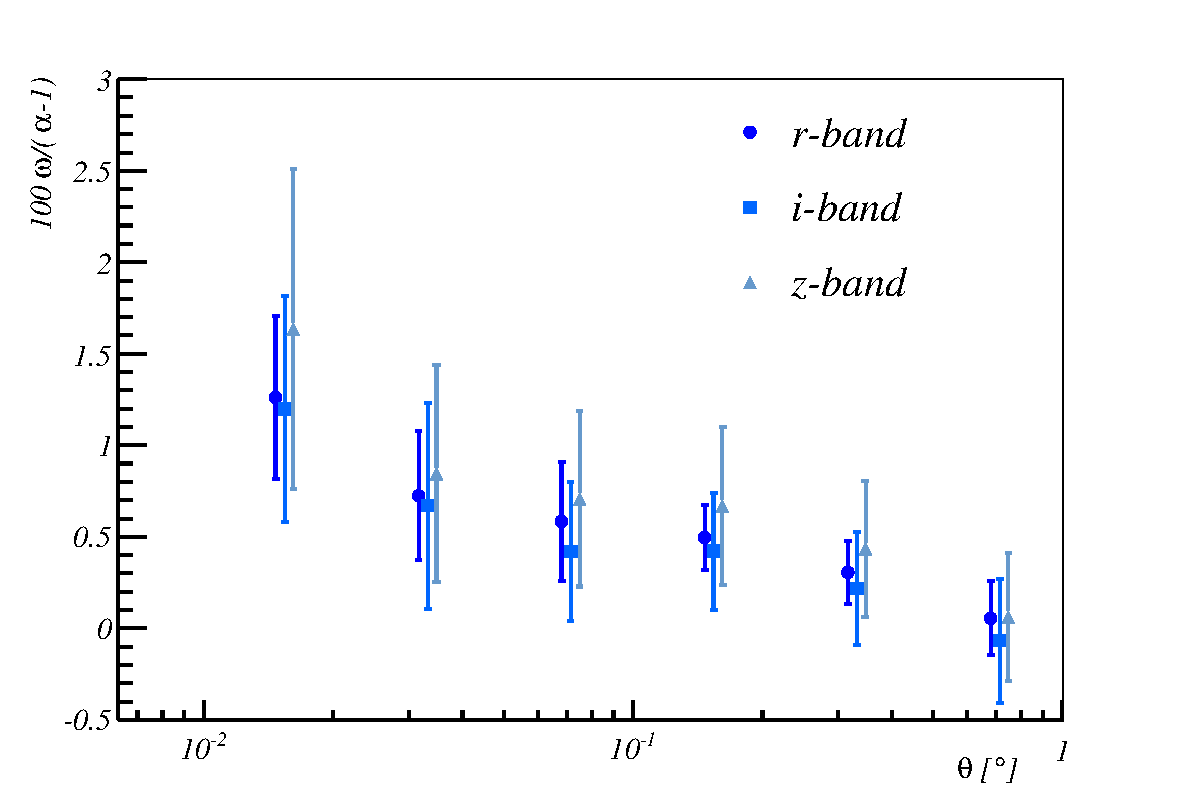
\includegraphics[width=0.85\textwidth]{./figures/acromatic_short.pdf}
\caption{Example of the achromaticity of the measured signal. Here are shown the measured two-point angular cross-correlation functions for $r<22.5$, $i<22.0$ and $z<21.5$ divided by their corresponding $\alpha-1$.}
\label{fig:achrom}
\end{center}
\end{figure}
\newline
 
 Finally, in order to test that the signal is achromatic, the measured two-point angular cross-correlation functions for each band, normalized by its $\alpha_S(m)-1$ are compared. All cross-correlation functions fluctuate within $1\sigma$ errors (see \autoref{fig:achrom} for an example) demonstrating that the measured convergence field does not depend on the considered band.

\subsection{Systematic error analysis}
\label{sec:sys}
Here, the impact of potential sources of systematic errors on the measured two-point angular cross-correlation function is investigated and how they are taken into account in the measurement is described.

\subsubsection{Number count slope $\alpha$}
    
\begin{figure}
\begin{center}
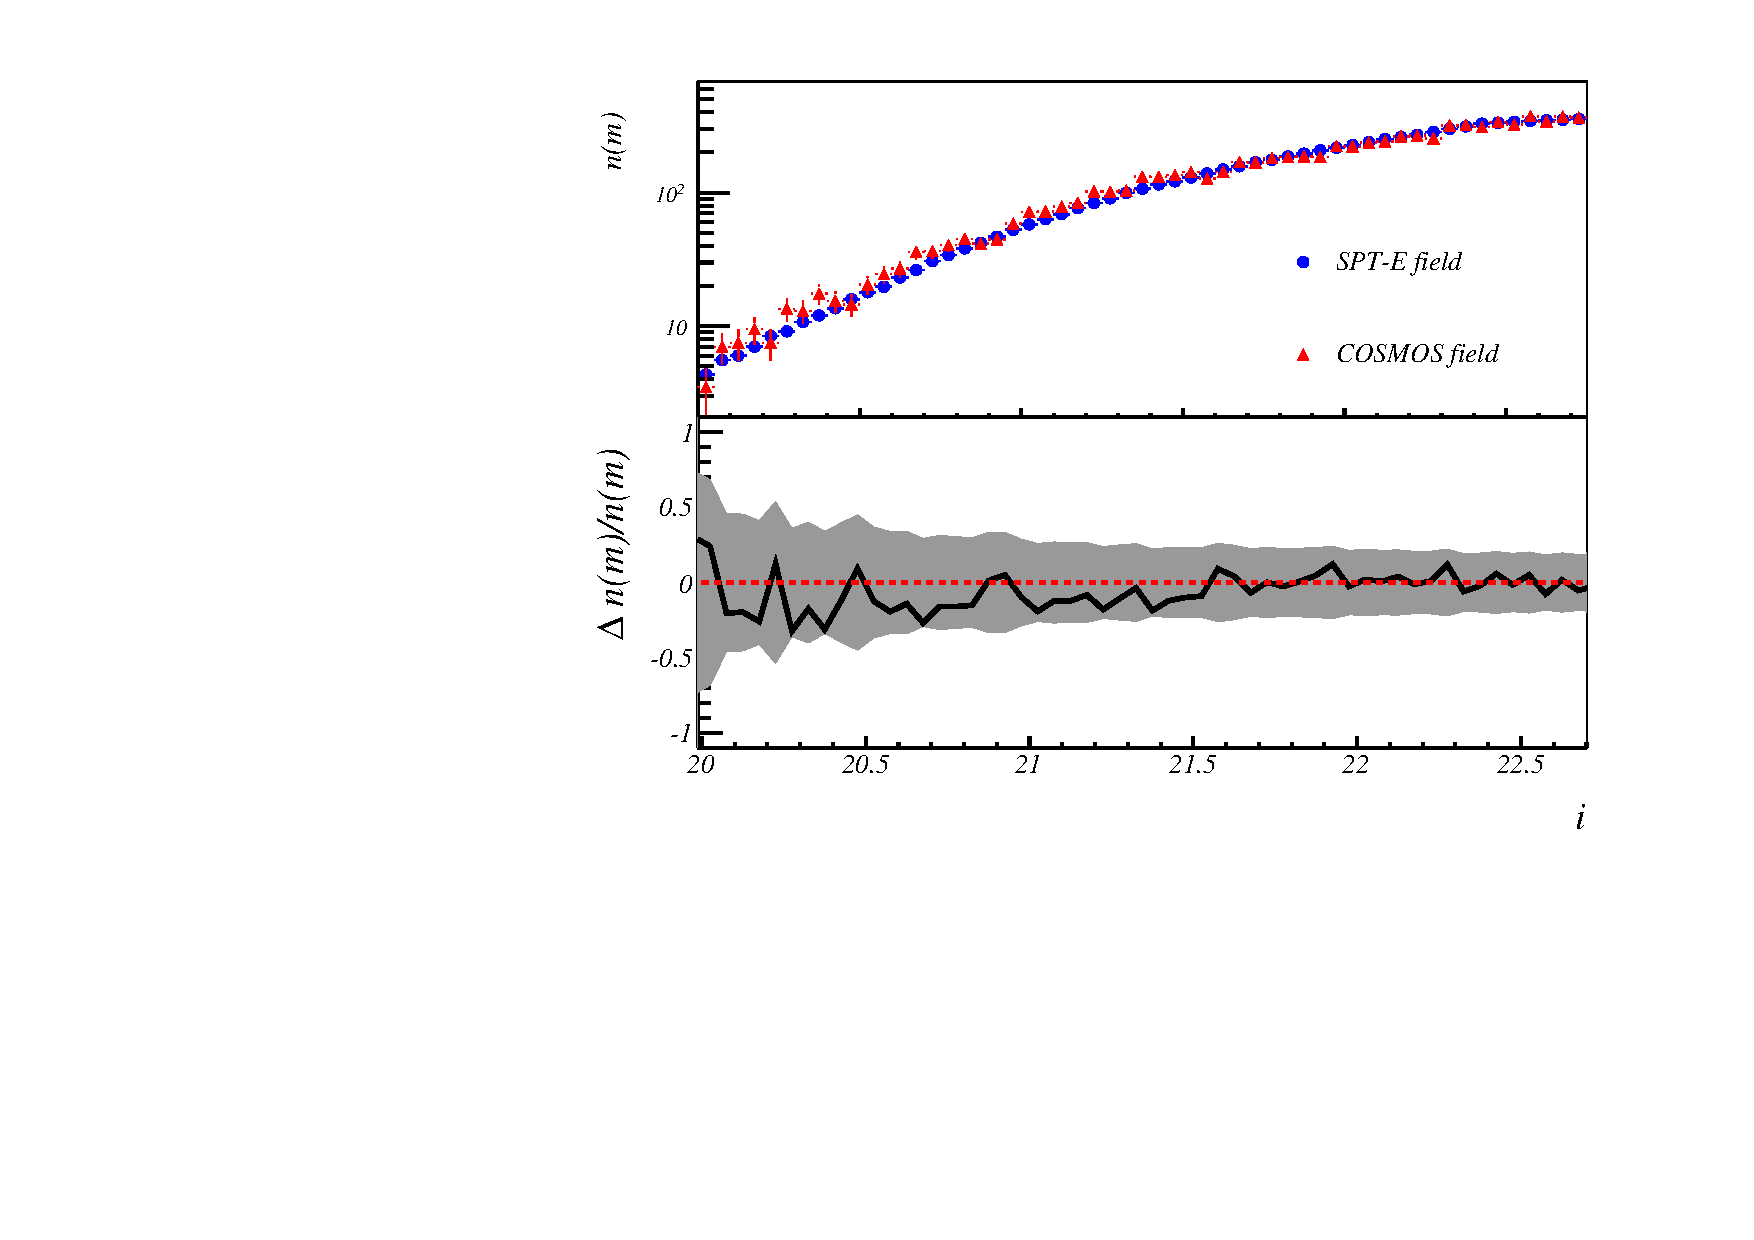
\includegraphics[width=0.85\textwidth]{./figures/SPTE_SNe.pdf}
\caption{Upper panel: Comparison of the magnitude distribution for the SPT-E and the COSMOS fields. Both histograms are normalized by their respective area. Lower panel: Relative difference between the magnitude distribution of the COSMOS and the SPT-E fields. The shaded region shows the $1\sigma$ confidence interval computed from shot-noise.}
\label{fig:ndmSN}
	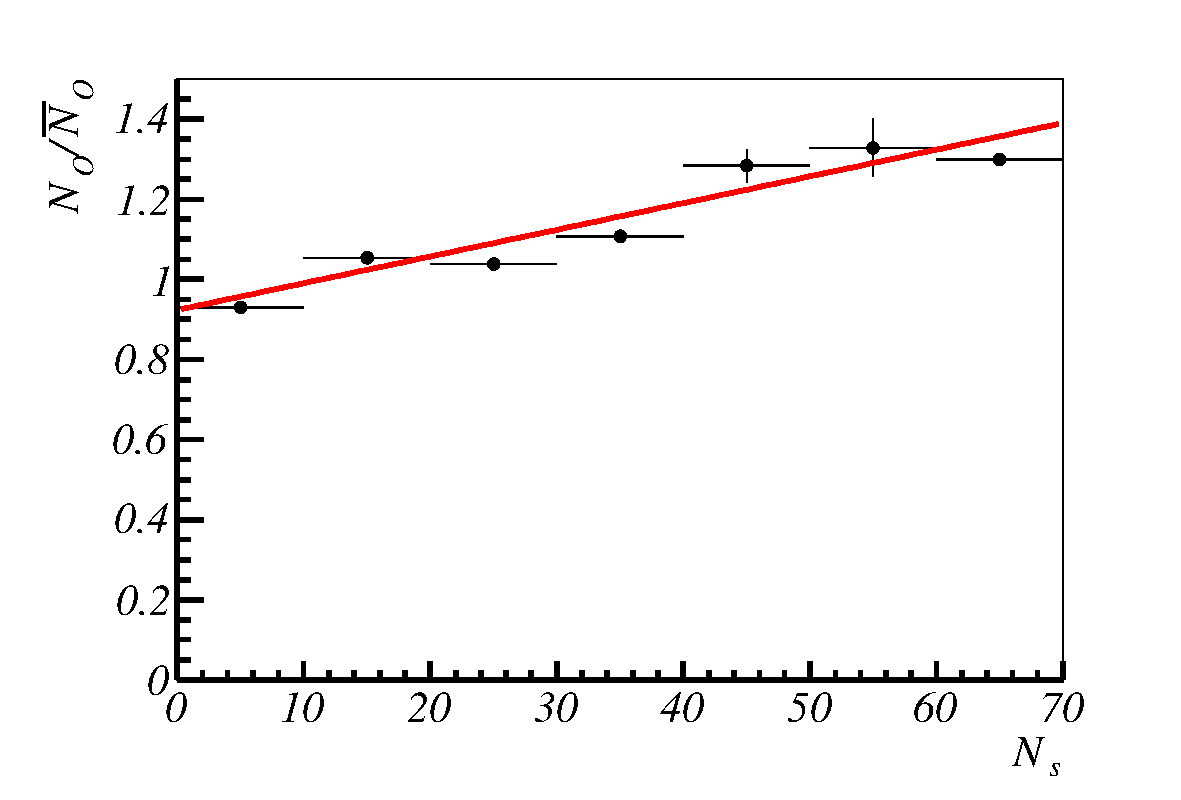
\includegraphics[width=0.85\textwidth]{./figures/purity_lens.pdf}
    \caption{Determination of the purity of the lens sample. For each $N_{\rm nside}=512$ {\scshape HEALPix}-pixel, the number of objects classified as galaxies divided by the average number of galaxies per pixel is plotted as a function of the  number of objects classified as stars. Black dots are the measured data. Red line is the linear fit to the data. The intercept of the line with the Y-axis is the estimated purity of the sample.}
    \label{fig:purity}
    \end{center}
\end{figure}
	When comparing the measured two point angular cross-correlation functions with the theoretical prediction via \autoref{eq:kappa_nc} for a given set of cosmological parameters, $\alpha(m)$ is determined by fitting the cumulative number count distribution to \autoref{eq:sch} and then using \autoref{eq:alpha}. To compute the possible impact of the uncertainty of this fit on the comparison with theory, a marginalisation over all the parameters of fit ($A,m_*,\beta$) is made.
\newline
	
Parameters are randomly sampled with a Gaussian distribution centerd on the value given by the fit to the cumulative number count and with a standard deviation equal to the $1\sigma$ errors of the fit. The value of $\alpha$ is recalculated with these randomly sampled parameters. The impact of the dispersion of the $\alpha$ values obtained is negligible compared to the size of the jackknife errors, so they are not taken into account.
\newline

In addition to the parameter determination, a possible non-completeness on the SPT-E field can modify the magnitude distribution altering the cumulative number count slope parameter \cite{2016MNRAS.455.3943H}. To estimate the possible impact of non-completeness, the measured magnitude distributions of the SPT-E field are compared with those of deeper fields measured by DES, such as the COSMOS field. Both distributions are found to be equal at the range of magnitudes considered on this analysis (see \autoref{fig:ndmSN} for an example in the $i$-band).

\subsubsection{Object obscuration}

Chang \cite{0004-637X-801-2-73} studied whether moderately bright objects in crowded environments produce a decrease in the detection probability of nearby fainter objects at scales $\theta\lesssim10\ $arcsec. However, such scales are well below those considered in this analysis ($\theta>36$ arcsec) and therefore this effect is ignored.

\subsubsection{Stellar contamination}
    
	For a given choice of star-galaxy classifier, there will be a number of stars misclassified as galaxies, so the observed two-point angular cross-correlation function $\omega_O(\theta)$ must be corrected by the presence of any fake signal induced by stars (see \cref{sec:starscorrection}):
	\begin{equation}
	\omega_{\rm LS_j} = \frac{\omega_{\rm O}(\theta)-\lambda_{\rm L}\omega_{\rm *S_j}(\theta)-\lambda_{\rm S_j}\omega_{\rm L*}(\theta)}{1-\lambda_{\rm L}-\lambda_{\rm S_j}},
	\label{eq:starcorrection}
	\end{equation}
	where $\omega_{\rm LS_j}$ is the corrected galaxy cross-correlation function, $\omega_{\rm L*}$ is the cross-correlation function of the true galaxy lenses with the stars misclassified as galaxies in the source sample, $\omega_{\rm *S_j}$ is the cross correlation of the stars misclassified as galaxies in the lenses with the true source galaxies and $\lambda_{\rm L},\lambda_{\rm S_j}$ are the fraction of stars in the lens and in the source samples respectively.
	Assuming that the misclassification of stars is spatially random and is a representative sample of the spatial distribution of the population classified as stars and that the fraction of misclassified stars is small, the functions $\omega_{\rm L*},\omega_{\rm *S_j}$ are estimated from the cross-correlation of the galaxy population and the stellar population in the corresponding redshift bin.
    \begin{sidewaysfigure}
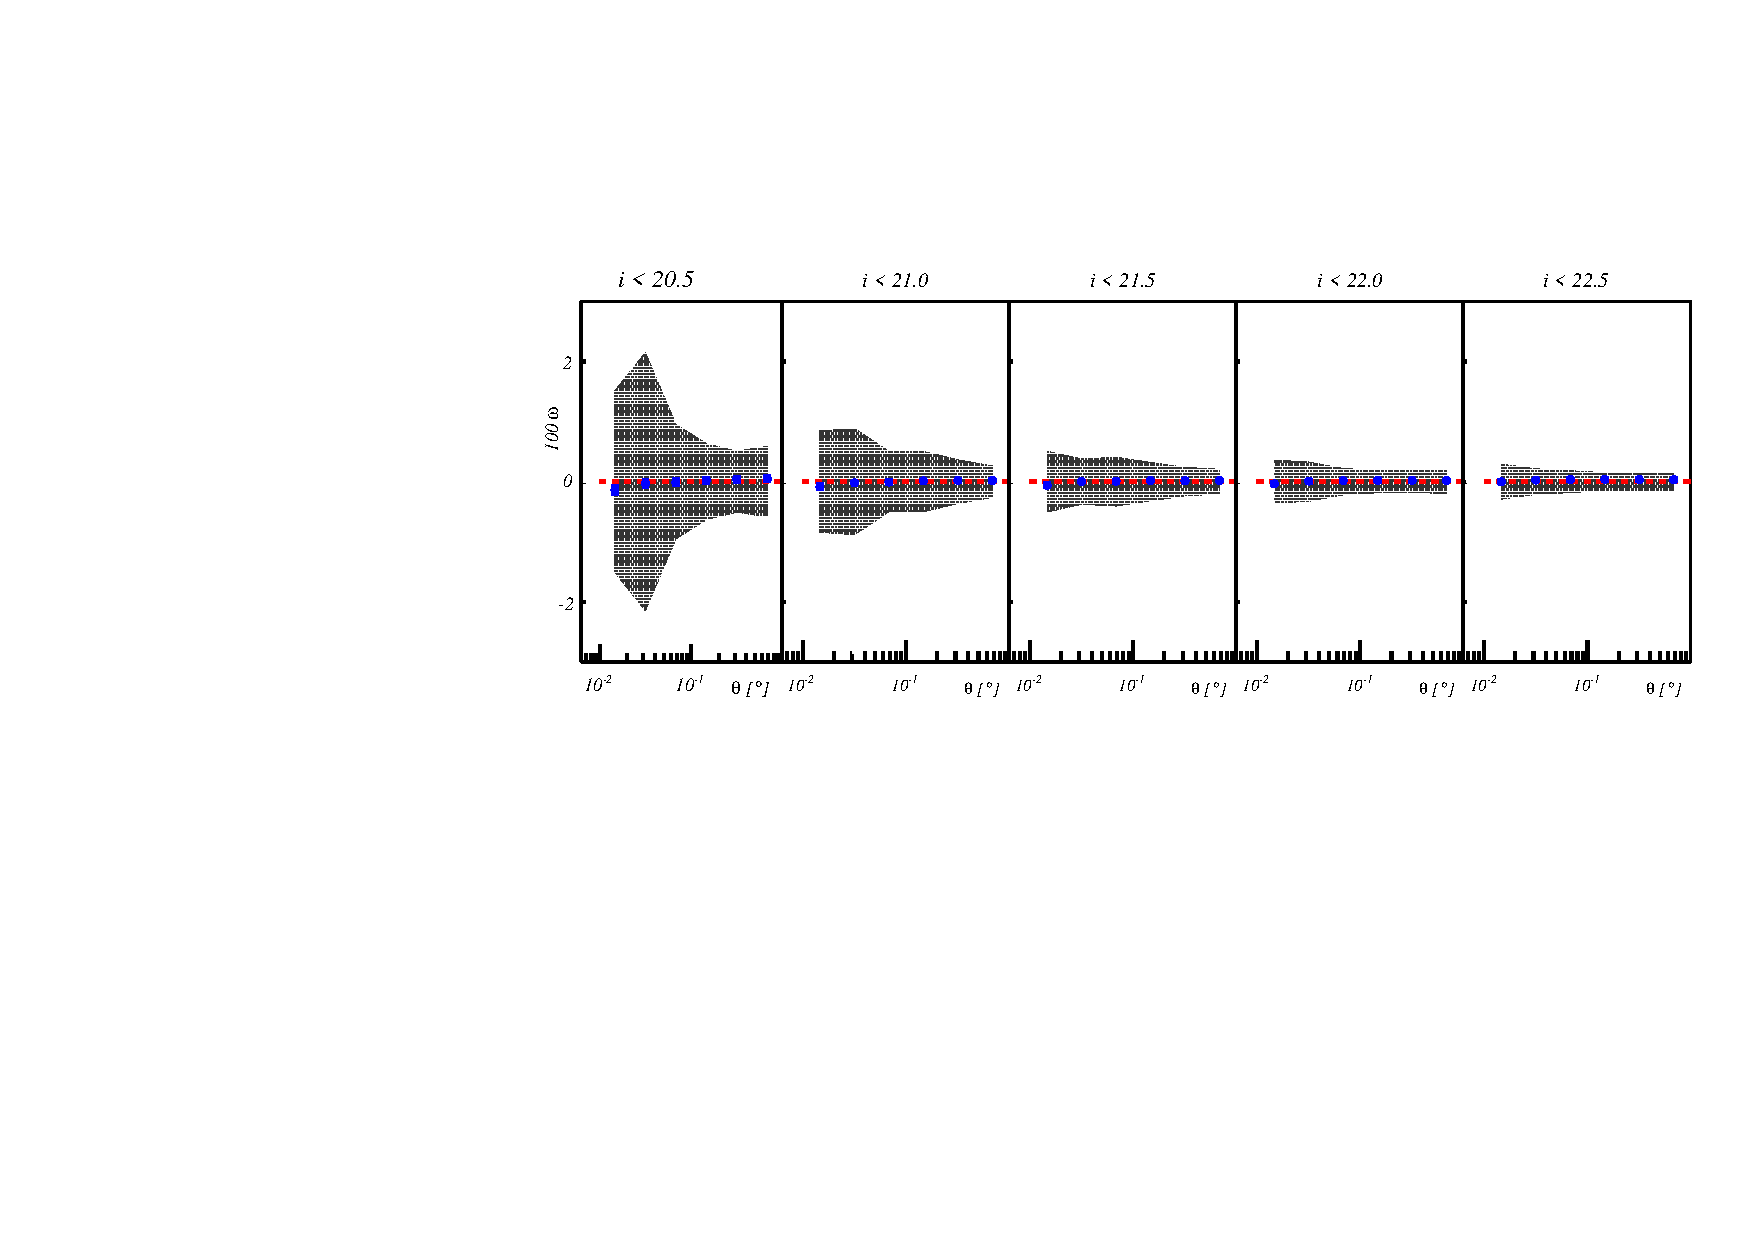
\includegraphics[width=\textwidth,trim={0 2.3cm 0 3.5cm},clip]{./figures/mag_istars.pdf}
\caption{Correction by stellar contamination on the $i<21.5$ sample. Blue dots are the correction and shaded area is the $1\sigma$ confidence interval of the measured cross-correlations of the magnification signal. Red dashed line is and eye-guide for zero.}
\label{fig:correction}
\end{sidewaysfigure}
\newline
 
	Following a similar approach to \cite{2012MNRAS.424..564R}, if the latter is true and the misclassified stars trace the global population of stars, for a given patch of the sky the number of objects classified as galaxies $N_{\rm O}$ must be the average number of true galaxies $\bar N_{\rm g}$ plus a quantity proportional to the number of stars on that given pixel,
	\begin{equation}
	N_{\rm O} = \bar N_{\rm g}+\tilde\gamma N_{\rm s}.
	\end{equation}
	Dividing by the average number of objects marked as galaxies $\bar N_{\rm O}$,
	\begin{equation}
	\frac{N_{\rm O}}{\bar N_{\rm O}} = p+\gamma N_{\rm s},
	\label{eq:purity}
	\end{equation}
	where $p=\bar N_{\rm g}/\bar N_{\rm O}$ is the purity of the sample, that is, $\lambda = 1-p$.
	\newline
	
	In order to estimate the purity of the galaxy sample with this method, an $N_{\rm side}=512$ {\scshape HEALPix} pixelation is made and for each pixel $N_{\rm O}/\bar N_{\rm O}$ and $N_{\rm s}$ is computed. Then, a fit to \autoref{eq:purity} is made determining a purity of 94 per cent for the lens sample and about 98 per cent for the source sample depending on the considered band (see \autoref{fig:purity} for an example). With this purity, the correction due to stellar contamination given by \autoref{eq:starcorrection} is found to be one order of magnitude smaller than the statistical errors (see \autoref{fig:correction} for the $i$-band correction), so stellar contamination is not taken into account in the analysis. Nevertheless, on future analysis with more galaxies and area this may be important. Note that the objects labeled as stars by our star-galaxy classifier would be a combination of stars and galaxies thus these calculations are an upper bound to stellar contamination.

	\subsubsection{Survey observing conditions}
    \label{sec:balrog}
    Observing conditions are not constant during the survey, leading to spatial dependencies across the DES-SV footprint \cite{2015arXiv150705647L} that may affect the observed cross-correlation function, such as seeing variations, air-mass, sky-brightness or exposure time \cite{2015MNRAS.454.3121M}. To trace these spatial variations, the catalog produced by the Monte Carlo sampling code {\scshape Balrog} has been used as random sample \cite{2016MNRAS.457..786S}. It is important to remark that {\scshape Balrog} catalogs are produced with the same pipeline as DES-SV data, allowing one to trace subtle effects such as patchiness on the zeropoints, deblending and possible magnitude errors due to a wrong sky subtraction close to bright objects.
    \newline
    
    The {\scshape Balrog} catalogs are DES-like catalogs, where
no intrinsic magnification signal has been included. The {\scshape Balrog} software generates images of fake objects, all with zero convergence $\kappa$, that are embedded into the DES-SV coadd images
(convolving the objects with the measured point spread function, and applying the measured photometric calibration). Then {\scshape SExtractor} was run on them, using the same DES Data Management configuration parameters used for the image processing. The positions for the simulated objects were generated randomly over the celestial sphere, meaning that these positions are intrinsically unclustered. Hence, the detected {\scshape Balrog} objects amount to a set of random points, which sample the survey detection probability. For a full description and an application to the same measurement as in \cite{2016MNRAS.455.4301C} see \cite{2016MNRAS.457..786S}. This is the first time that this extensive simulation is used to correct for systematics. The same cuts and masking of the data sample (\autoref{sec:data_sample_SV}) are also applied to the the {\scshape Balrog} sample. A re-weighting following a nearest-neighbours approach was applied to {\scshape Balrog} objects in order to follow the same magnitude distribution of the DES-SV data on both lens and sources.
    \newline
    
     The use of Monte Carlo sampling methods provides a new approach to mitigate systematic effects complementary to methods that cross-correlate the galaxy-positions with the maps of the survey observing conditions \cite{2012MNRAS.424..564R,2012ApJ...761...14H,2015MNRAS.454.3121M} or involve masking the regions of the sky with worst values of the observing conditions \cite{2016MNRAS.455.4301C}. The amount of sky to be masked in order to mitigate the systematic effects on the correlation functions, is freely decided based on the impact on the correlation function, which may lead to a biassed measurement. On the other hand, the approach involving cross-correlations may lead to an overcorrection effect since the different maps of the observing conditions are, in general, correlated in a complicated manner \cite{2016MNRAS.456.2095E}. This new Monte Carlo technique to sample the selection function of the survey given by {\scshape Balrog}, has the advantage that takes into account the correlation of the different observing conditions maps as well as provides an objective criteria to mitigate systematic errors on the correlation function for a given sample, avoiding biassed measurements. In addition, the use of {\scshape Balrog} has the potential to allow us in the future to exploit the full depth of the survey \cite{2016MNRAS.457..786S}.
\newline

{\scshape Balrog} allows to explore how the {\it real} properties of the galaxies are mapped into the observed ones. One might think that it may be translated from observed to real quantities. This is not possible since that although the $real\rightarrow observed$ map is one-to-one, meanwhile the $observed\rightarrow real$ is not.
\newline

Although the use of {\scshape Balrog} is a ground-breaking technique on the mitigation of systematic errors, its limitation must be taken into account. The simulated catalogs are as good as the input catalogs are an accurate representation of the reality. Thus, if an specific population of galaxies is not on the input, it will not be taken into account. DES-SV {\scshape Balrog} catalogs are based on the {\scshape COSMOS} survey\footnote{cosmos.astro.caltech.edu}, that is based on images from the Hubble Telescope that are deeper than the DES survey. Thus, the overall quality of the input catalog is better than DES. Thus this should not be a limitation on this analysis.

\subsubsection{Dust extinction}
\label{sec:dustext}

\begin{sidewaysfigure}
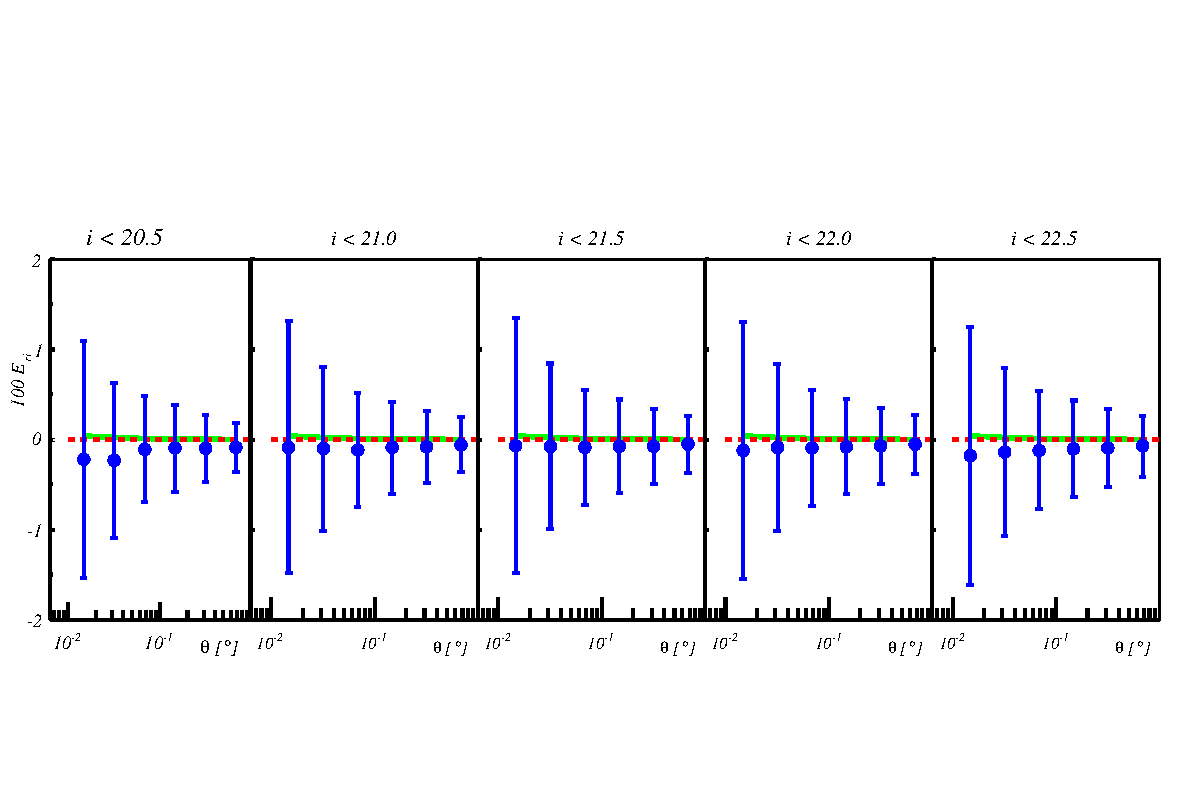
\includegraphics[width=\textwidth,trim={0 2.3cm 0 3.5cm},clip]{./figures/mag_i_ri.pdf}
\caption{Blue dots: color-density cross-correlation functions measured on SV data for the {\it r} and {\it i} bands (sample $i<21.5$). Green solid line is the expected value from \autoref{eq:colorexcess}. Red dashed line is an eye-guide for zero.}
\label{fig:colorexcess}
\end{sidewaysfigure}

\begin{sidewaysfigure}
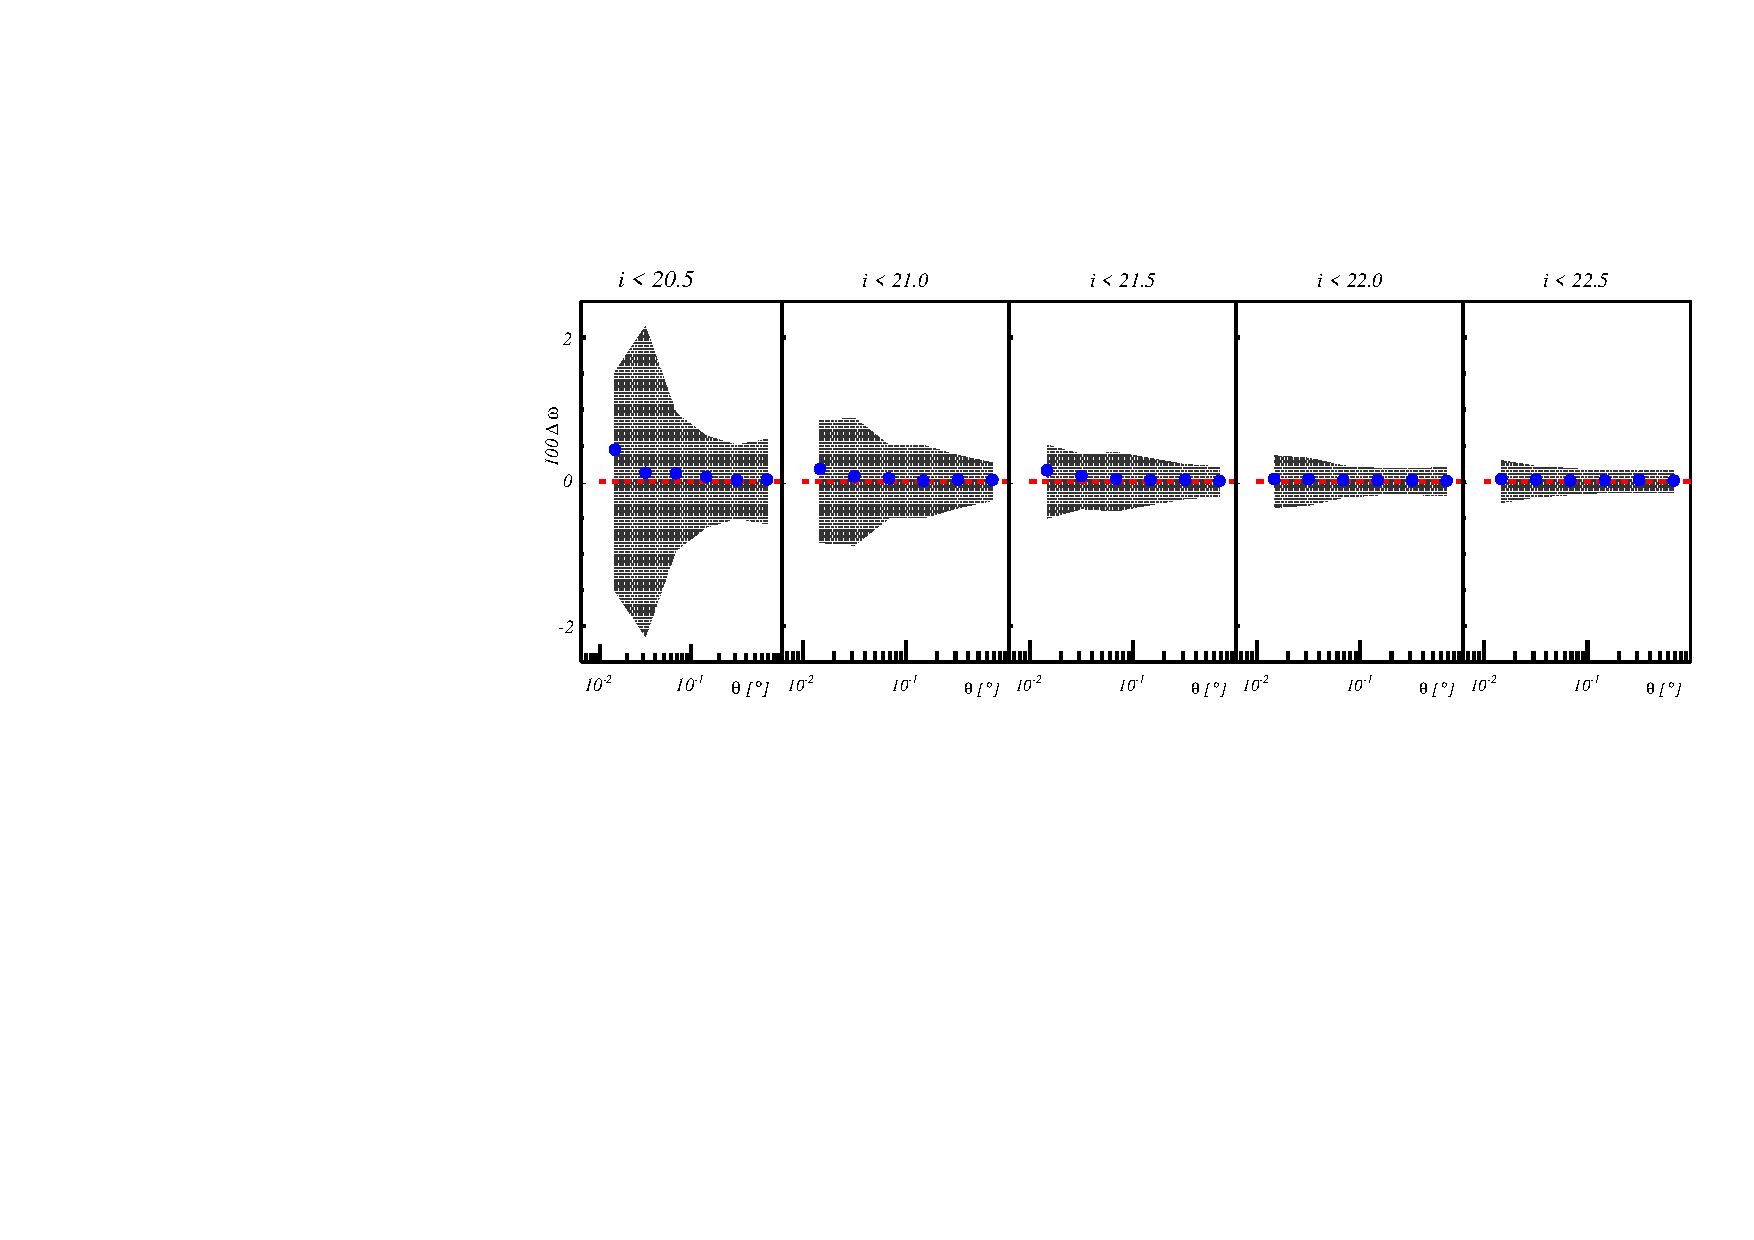
\includegraphics[width=\textwidth,trim={0 2.3cm 0 3.5cm},clip]{./figures/mag_idust.pdf}
\caption{Impact of dust on the number count from MICE (sample $I$). Shade is the $1\sigma$ confidence interval. Blue dots are the number count differences between the case with and the case without the simulated dust profile. Red dashed line is an eye-guide for zero.}
\label{fig:micedust}
\end{sidewaysfigure}
The possible presence of dust in the lenses may modify the observed magnitude in addition to the magnitude shift due to magnification \cite{2010MNRAS.405.1025M}. The change in magnitude ($\delta m$) on the $p$-band may be written as
\begin{equation}
\delta m_p = -2.5\log\mu+\frac{2.5}{\ln10}\tau_p,
\end{equation}
where  $\mu\simeq1+2\kappa$ is the change in magnitude due to magnification and $\tau_k$ is the optical depth due to dust extinction. Whereas magnification is achromatic, dust extinction induces a band-dependent magnitude change. Taking this into account, the color-excess for bands $p,q$\footnote{In this section $p,q$ stand for a generic index label while $V$ stands for the $V$ band of the $UBV$ system.} is defined as
\begin{equation}
E_{pq} = \delta m_p-\delta m_q=1.08[\tau_p-\tau_q].
\end{equation}
Define the color-density cross-correlation as \cite{2010MNRAS.405.1025M}
\begin{equation}
\langle \delta_{\rm g}E_{pq}\rangle(\theta) = 1.09[\tau_p(\theta)-\tau_q(\theta)],
\end{equation}
where $\delta_{\rm g}$ is the density contrast of the lenses and $E_{pq}$ is the color-excess of the sources; from the measurements by \cite{2010MNRAS.405.1025M} it can be parametrized as
\begin{equation}
\langle\delta_{\rm g}E_{pq}\rangle(\theta) = 1.09\tau_V\left[\frac{\lambda_V}{\lambda_p}-\frac{\lambda_V}{\lambda_q}\right]\left(\frac{\theta}{1'}\right)^{-0.8},
\label{eq:colorexcess}
\end{equation}
with $\tau_V=2.3\times10^{-3}$ the optical depth at the {\it V}-band  and $\lambda_V,\lambda_p,\lambda_q$ the average wavelengths of the $V$, $p$ and $q$ bands respectively. With this parametrization, the impact of dust extinction is negligible at the scales considered on this analysis. As it can be seen in \autoref{fig:colorexcess}, color-density cross-correlation functions are compatible with \autoref{eq:colorexcess} as well as with zero.
\newline

In addition, the impact of a dust profile has been simulated as described in \autoref{eq:colorexcess} with the MICE simulation (\autoref{sec:mice}). To do so, for each galaxy belonging to the source sample a magnitude shift is induced
\begin{equation}
m_d = m_\mu +1.09\tau_V\frac{\lambda_V}{\lambda}\sum\limits_{l}\left(\frac{\theta_l}{1'}\right)^{-0.8}.
\end{equation}
Here $\theta_l$ is the angular separation of the source-galaxy and the $l$-th lens galaxy and the summation is over all the galaxies of the lens sample. In \autoref{fig:micedust} the difference between the two-point angular cross-correlation with and without the dust can be seen to be less than the statistical errors. It can be deduced that dust has no impact on the angular scales considered on this work.
\newline

Since the parametrization used here only applies to a sample similar to the one used at \cite{2010MNRAS.405.1025M}, statements about dust constrains are limited. Nevertheless this does not change the fact that no chromatic effects are detected.

\subsubsection{Photometric redshifts}

\begin{figure}
%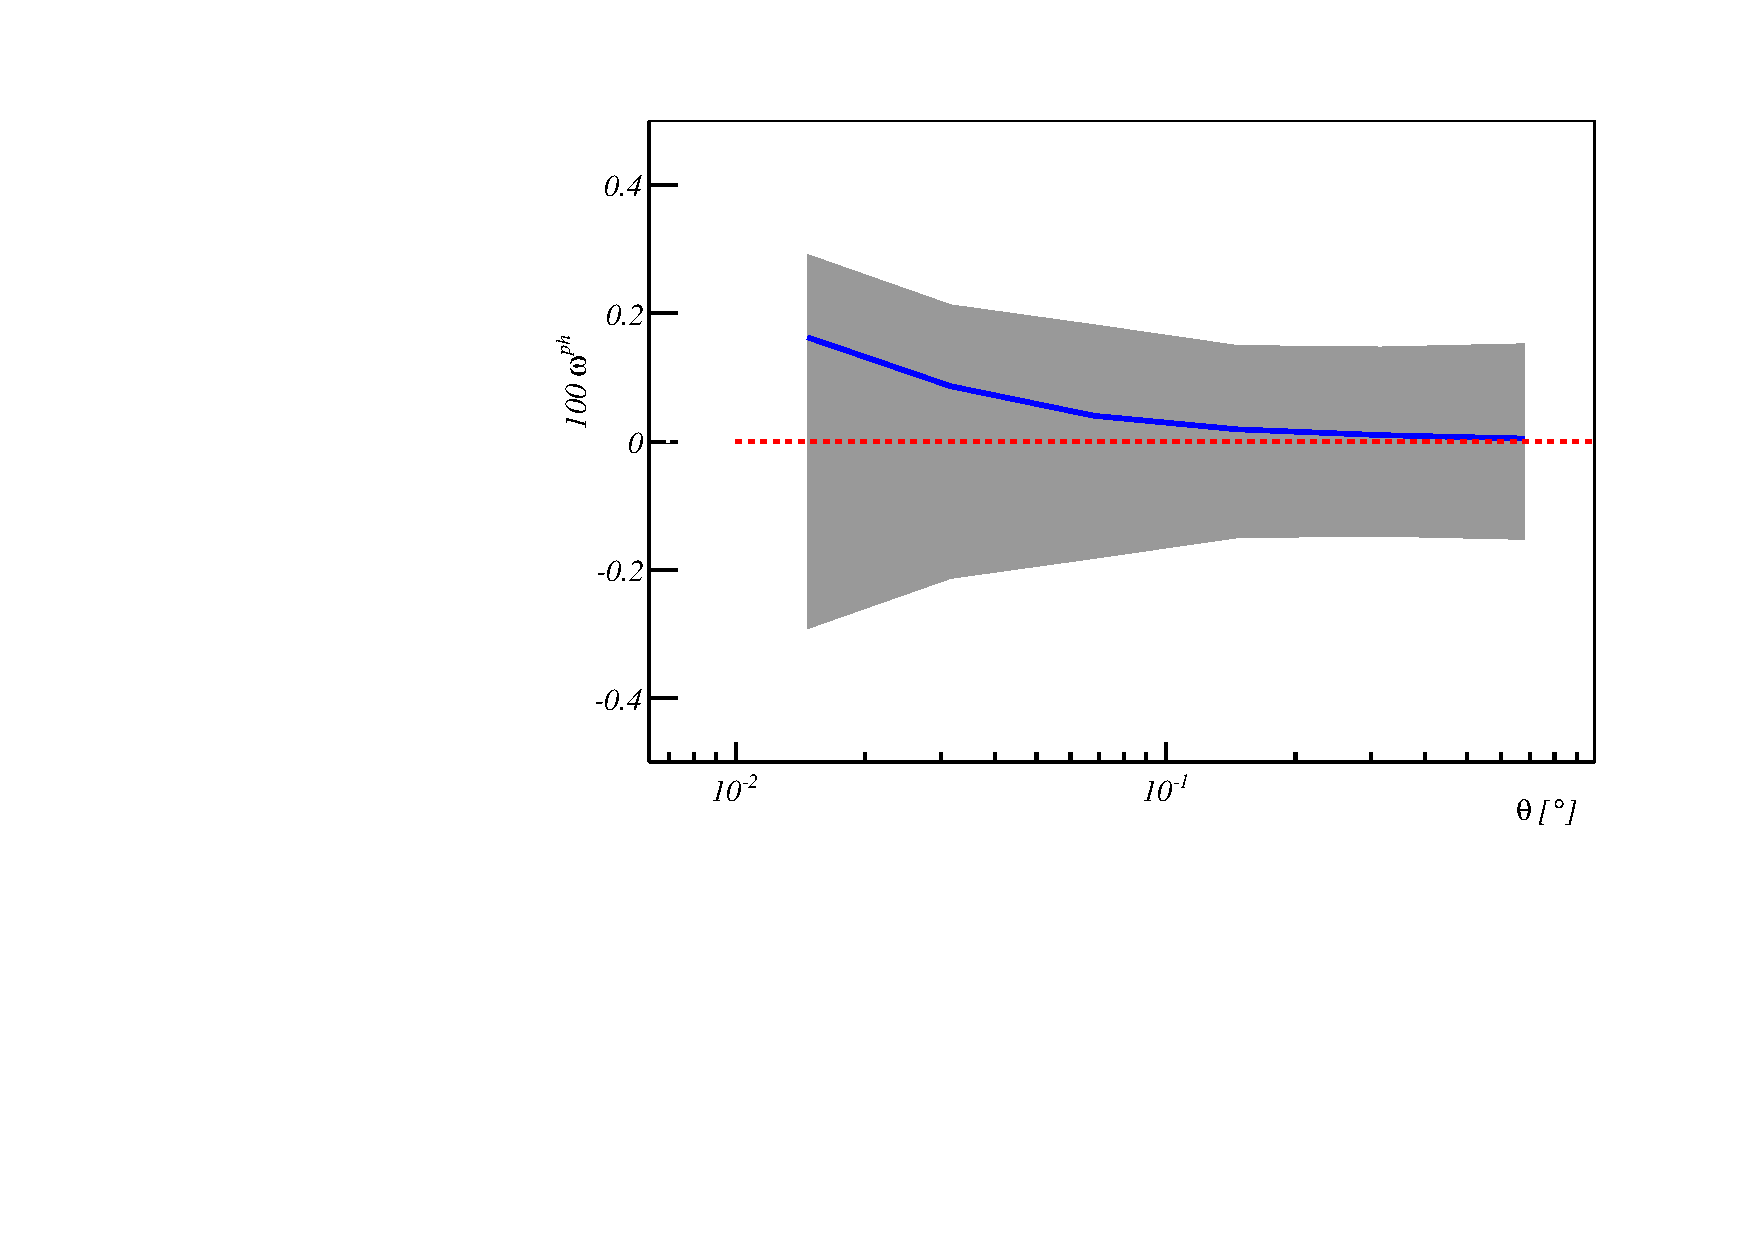
\includegraphics[width=0.5\textwidth]{./figures/mag_itheo_photoz_short.pdf}
\caption{Comparison of $1\sigma$ jackknife errors of the measured correlation function (grey shade) with the expected signal induced by the photo-z migration between the lens and the source sample (sample $I$) computed theoretically with the stacking of the pdfs for the $i$-band (blue line).}
\label{fig:theophotoz}
\end{figure}

A general study of photo-z performance in DES-SV can be found in \cite{2014MNRAS.445.1482S}. A comprehensive study of the photo-z performance and its implications for weak lensing for this data can be found in \cite{PhysRevD.94.042005}. Both studies are followed in this analysis.
\newline
	Conservative photo-z cuts are made in order to minimize migration between lens and source samples. Nevertheless, catastrophic outliers in the photo-z determination can bias the measurement of  $\kappa$ \cite{2010MNRAS.401.1399B}. Thus, the tails of the probability density functions (pdfs) of the photo-z code are a crucial systematic to test.
	\newline
	As mentioned in \autoref{ch:theory}, in addition to the magnification signal, galaxy migration due to a wrong photo-z assignment between lens and source samples may induce a non-zero cross-correlation signal due to the physical signal coming from the clustering of objects in the same redshift bin. As a first approach, estimation of the expected signal induced by photo-z migration ($\omega^{ph}$) is computed with \autoref{eq:4t}:
\begin{equation}
\omega_{\rm LS_j}^{\rm ph}(\theta) = \int\limits_0^\infty dz\int\limits_0^\infty dz' \phi_{\rm L}(z)\phi_{\rm S_j}(z')\xi(\theta;z,z'),
\label{eq:phth}
\end{equation}
where $\xi(\theta;z,z')$ is the 3D correlation-function and $\phi_{\rm L},\phi_{\rm S_j}$ are the redshift distribution of the lens (L) sample and the source sample ($\rm S_j$) estimated from the stacking of the pdfs given by TPZ. \autoref{fig:theophotoz} compares the measured two-point angular cross-correlation and the expected signal induced by photo-z can be seen for the \textit{I} sample. The signal induced by photo-z is found to be smaller than the statistical errors. Note that this method relies on an assumed cosmology and bias model, and therefore should be considered only an approximation. A more accurate calculation can be made with the help of N-body simulations.
\newline

From the overlap of the redshift distribution of both lens and source samples, it is found that the total photo-z migration between lens and source sample is $o\sim 0.6\%$ depending on the magnitude cut of the source sample. The procedure to compute this overlap is to integrate the product of the pdfs of the lens and source sample:
\begin{equation}
o = \int\limits_0^\infty dz\phi_L(z)\phi_S(z),
\end{equation}
where $\phi_L,\phi_S$ are the stacked pdfs of the lens and source sample respectively. Since TPZ provides an individual pdf for each galaxy, the stacked pdf of a given sample is computed by adding all the individual pdfs of the galaxies that belong to that sample (see \cite{2016MNRAS.459.1293A} for a study of clustering with stacked pdfs).
\newline

To estimate the maximum photo-z migration allowed between the lens and the source sample, the MICE simulation (\autoref{sec:mice}) with the un-lensed coordinates and magnitudes is used. Galaxies are randomly sampled on the lens redshift bin and then placed on the source redshift bin. Conversely, galaxies on the source redshift bin are randomly sampled and placed on the lens redshift bin. For a given lens or source sample, the number of galaxies introduced from the other redshift bin is chosen to be 0.1, 0.3, 0.5, 0.7, 0.9 and 2 per cent of the galaxies. Then, the two-point angular cross-correlation is computed for each case. The difference of the correlation functions measured at the simulation with induced migration between lens and source sample and the original used in \autoref{sec:mice} is the signal induced by photo-z migration. The signal induced by photo-z for the cases with 0.9 and 2 per cent computed with this method can be seen at \autoref{fig:photozcontamination}. It is found that  at 0.9 per cent of contamination, the induced signal due to photo-z migration is comparable to the error in the correlation functions. This upper limit is greater than the estimated photo-z migration, demonstrating that the effect of photo-z migration is negligible. Photo-z migration has a larger impact on the brightest samples. Nevertheless, since the errors of the correlation functions of these samples are shot-noise dominated, the tightest constrains on photo-z migration are imposed by the faintest samples. With a larger data sample this statement will no longer be true.
\begin{sidewaysfigure}
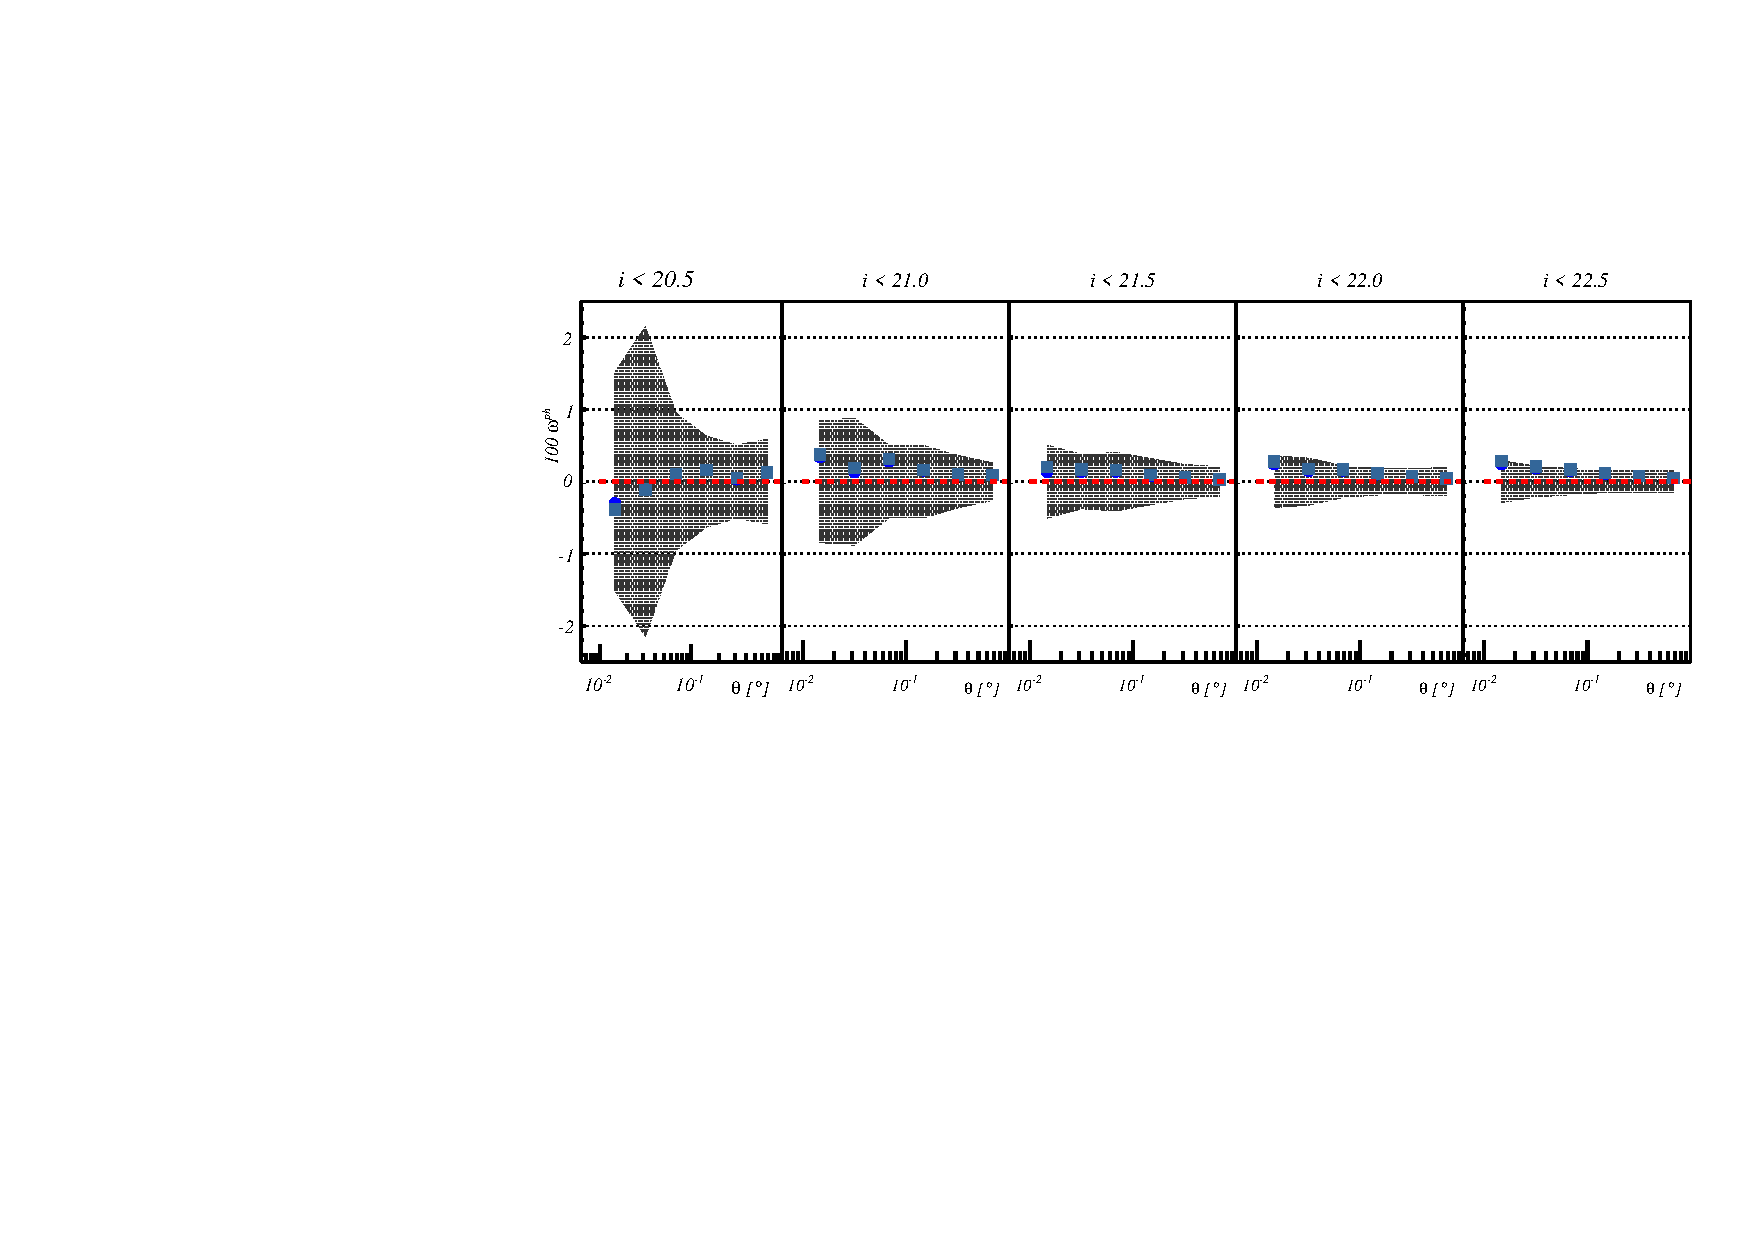
\includegraphics[width=\textwidth,trim={0 2.3cm 0 3.5cm},clip]{./figures/mag_i_mix.pdf}
\caption{Estimation of the signal induced by migration of selected fractions of MICE un-lensed galaxies between the lens and the source sample (sample $I$). Shaded area is the $1\sigma$ confidence interval for the measured number count cross-correlations. Dark blue dots correspond to a contamination fraction of 0.9 per cent. Violet squares correspond to a 2 per cent. Squares are displaced at the X axis for clarity. Red dashed line is an eye-guide for zero.}
\label{fig:photozcontamination}
\end{sidewaysfigure}
\newline

Photo-z induced correlation functions that mimic magnification may affect the measured significance. Thus, Bayes factor is recomputed with two new hypothesis, the measured signal is a combination of magnification and photo-z ($M+Ph$) or the measured signal is only photo-z ($Ph$):
\begin{equation}
\mathcal{B} = \frac{P(M+Ph|\Theta)}{P(Ph|\Theta)} = \frac{P(\Theta|M+Ph)}{P(\Theta|Ph)},
\end{equation}
where
\begin{equation}
P(\Theta|M+Ph) = e^{-\chi^2_{\rm Planck+Ph}/2}
\end{equation}
and
\begin{equation}
P(\Theta|Ph) = e^{-\chi^2_{\rm Ph}/2}.
\end{equation}
To compute $\chi^2_{\rm Planck+Ph}$ and $\chi^2_{\rm Ph}$ it has been assumed that the expected theory is given by $\omega_{\rm LS_j}(\theta)+\omega_{\rm LS_j}^{\rm ph}(\theta)$ and $\omega_{\rm LS_j}^{\rm ph}$ respectively, where $\omega_{\rm LS_j}^{\rm ph}$ is the expected signal induced by photo-z computed using \autoref{eq:phth}. The significances recomputed using these two new hypothesis for the {\it r}, {\it i} and {\it z} bands are $\log_{10}\mathcal{B}=2.5, 4.0, 3.5$ respectively. Thus, it can be concluded that photo-z migration has a limited impact on the measured significances.
\newline

All previous calculations were based on the assumption that the pdfs are a reliable description of the true redshift distribution. This statement can be partially validated comparing the pdfs with the spectroscopic redshift distribution for the same sample (see \autoref{fig:specphotoz} for an example).  Redshift distributions predicted by TPZ are found to be representative of those given by the spectroscopic sample. Nevertheless, this statement has limitations --but is good enough for SV data-- and a more accurate description of the real redshift distribution of the full sample will be measured with methodologies involving clustering-based estimators \cite{2008ApJ...684...88N,2010ApJ...721..456M,2013arXiv1303.4722M,2016MNRAS.462.1683S} when the size of the data sample grows. This type of estimators involve the use of two-point angular cross-correlations between different redshift bins, whose measurement may be biassed by number count magnification itself. Nevertheless, as it has been stated in \autoref{ch:theory}, depending on the value of the number count slope, the amplitude induced by magnification on the correlation-function may be zero. Thus, when employing this kind of estimators, samples should be carefully chosen so that $\alpha_S-1=0$. This can be done by measuring the number count slope at the cumulative magnitude distribution with methods such that used in this work.
\begin{figure}
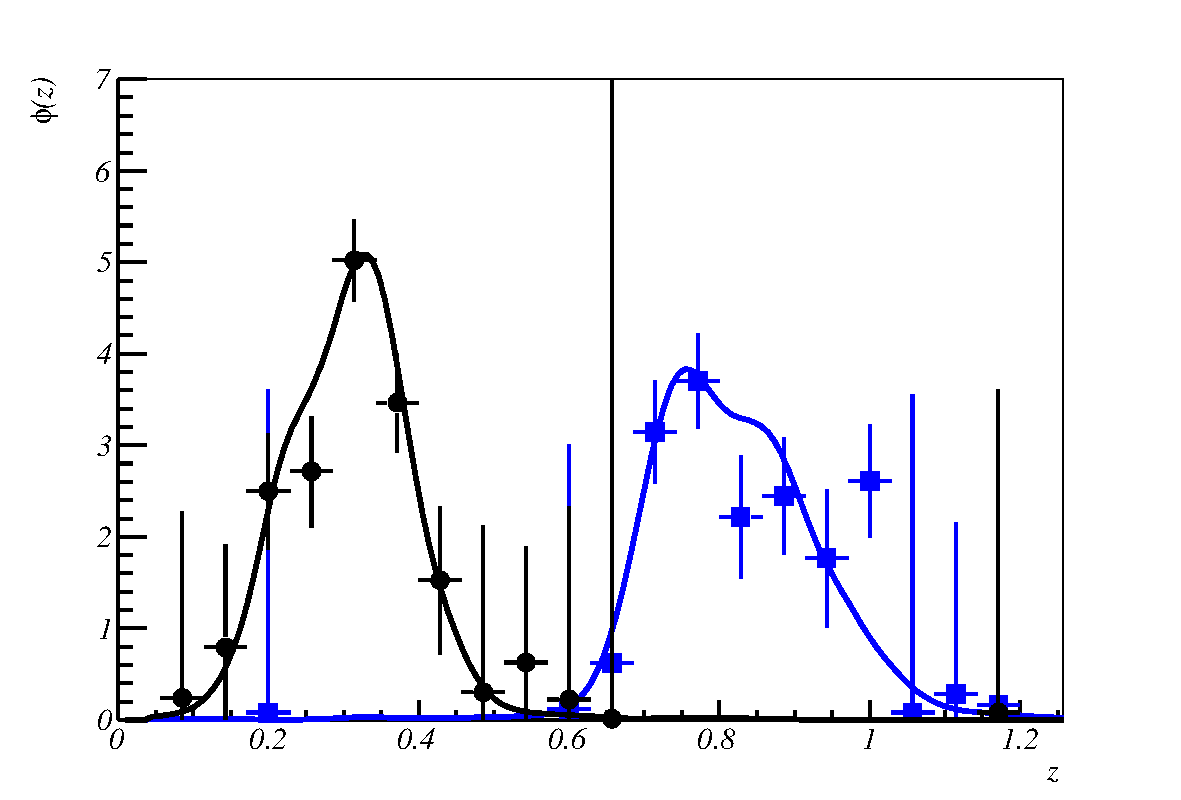
\includegraphics[width=\textwidth]{./figures/spec_photoz_cmp.pdf}
\caption{Comparison of the redshift distribution computed by the stacking of the pdfs given by TPZ ( solid lines) with the ones computed with the spectroscopic sample of the lens (black dots) and the source sample $i<22.5$ (blue squares).}
\label{fig:specphotoz}
\end{figure}
\newline

    Finally, to demonstrate that the measured signal is independent of the photo-z technique employed to estimate the redshift, the two-point angular cross-correlation functions used on this analysis are re-computed with redshift estimated with other two different approaches that have shown to have similar performance as TPZ \cite{2014MNRAS.445.1482S} a neural network, Skynet  \cite{2014MNRAS.441.1741G}, and a template based approach, Bayesian Photo-Z (BPZ) \cite{2000ApJ...536..571B}. \autoref{fig:bpzskynet} compares the cross-correlations computed with the three codes for the $i$-band, showing them to be within $1\sigma$ errors.
\begin{sidewaysfigure}
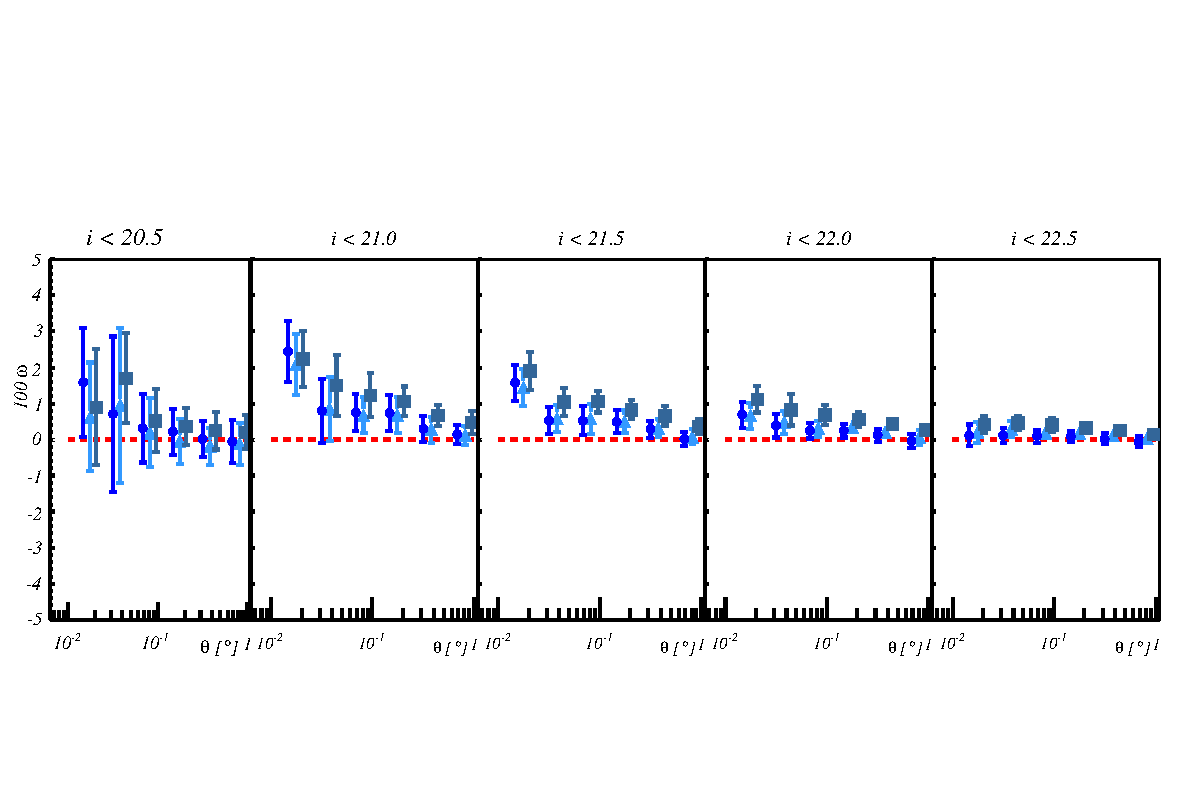
\includegraphics[width=\textwidth,trim={0 2.3cm 0 3.5cm},clip]{./figures/mag_i_photoz_comparison.pdf}
\caption{Comparison of the measured two-point angular cross-correlation functions corresponding to the sample $i<21.5$ measured with the Landy-Szalay estimator using TPZ, Skynet and BPZ. Triangles and squares are displaced at the horizontal axis for clarity.}
\label{fig:bpzskynet}
\end{sidewaysfigure}

\subsection{Discussion}
\label{sec:discussion_sv}

On this analysis, the weak-lensing magnification signal has been detected on the DES-SV data using the general population of galaxies. In addition, a thorough and detailed study of the possible systematic effects is made. The systematic error estimation has been made, for the first time, with the help of two simulations: MICE --a N-body-- and {\scshape Balrog} --an image simulation--.
\newline

From all of the systematic error estimation, two of them have shown to be critical for magnification on photometric surveys: the observing conditions and the photo-z migration between the lens and the source sample.
\newline

This analysis demonstrates that reliable weak-lensing magnification can be measured accurately for a galaxy survey such as DES, opening a whole new window to new physic analysis within the experiment.


\section{Magnification in DES Year 1 data}
\label{sec:y1data}
As the new data-release was available --the DES Year 1 (DES-Y1)-- on May 2016, with more area but less depth, the analysis started after this date were performed here. This new data-sample is much more numerous than DES-SV, allowing to do analyses that were impossible before with the Dark Energy Survey.
\newline

The goal of this analysis is to use the methodology to measure weak-lensing magnification signal developed at \autoref{sec:analysis_sv} to determine the convergence profile of voids and troughs with the DES-Y1 data. Data sample is described at \autoref{sec:data_sample_y1}. Then, the analysis is described and the results discussed at \autoref{sec:analysis_y1}. Finally a discussion on the analysis can be found at \autoref{sec:discussion_y1}.

\subsection{Data sample}
\label{sec:data_sample_y1}


\subsubsection{Lens sample}
Two lens samples

\subsubsection{Source sample}
The DES Y1-Gold main galaxy catalog, amounts 1600 deg$^2$ divided between several fields that include the supernovae fields, the stripe-82 (S82) and the SPT field (see \autoref{fig:des_y1_coverage}). From these fields, the largest contiguous area is selected, the SPT.
\newline

Regions with declination $ < -60^{\circ}$ are removed in order to avoid the Large Magellanic Cloud and severe stellar contamination from the Milky Way. {\scshape Modest\_class} is employed as star-galaxy classifier in combination with the additional morphological cut:
\begin{equation}
\mbox{spread\_model\_i} + \frac{5}{3}\mbox{spreader\_model\_i} > 0.007.
\end{equation}
\newline

The following color cuts are made in order to remove outliers in color space:
\begin{itemize}
	\item $-1 < g-r < 3$,
	\item $-1 < r-i < 2$,
	\item $-1 < i-z < 2$;
\end{itemize}
where {\it g}, {\it r}, {\it i}, {\it z} stand for the corresponding {\scshape mag\_auto} magnitude measured by {\scshape SExtractor}. Bad regions, and haloes around bright stars are also removed following the same criterias as in \autoref{sec:data_sample_SV}.
\newline

Depth cuts are also imposed on the {\it riz}-bands in order to have uniform depth when combined with the magnitude cuts. These depth cuts are reached by including only the regions that meet the following conditions:
\begin{itemize}
	\item $r_{\rm lim} > 22.5$,
	\item $i_{\rm lim} > 22.0$,
	\item $z_{\rm lim} > 21.0$;
\end{itemize}
where $r_{\rm lim}, i_{\rm lim},z_{\rm lim}$ stand for the magnitude limit in the corresponding band. The resulting footprint, as shown in \autoref{fig:footprint_y1}, after all the masking cuts amounts to $XXXX \mbox{ deg}^2$.
\newline

Photometric redshifts (photo-z) have been estimated using different techniques. In particular, the fiducial code used in this work employs a machine-learning algorithm (random forests) as implemented by TPZ \cite{2013MNRAS.432.1483C}, which was shown to perform well on SV data \cite{2014MNRAS.445.1482S}. The redshifts of the galaxies are defined according to the mean of the probability density functions given by TPZ ($z_{\rm ph}$). Other methods are also employed to demonstrate that the measured two-point angular cross-correlation are not a feature induced by TPZ.
\newline

Three source samples are defined, one per band:
\begin{itemize}
	\item R: $0.7 < z_{\rm ph} < 1.0$ and $r<22.5$;
	\item I: $0.7 < z_{\rm ph} < 1.0$ and $i<22.0$;
	\item Z: $0.7 < z_{\rm ph} < 1.0$ and $z<21.5$.
\end{itemize}

Following the same approach as in the \autoref{sec:svdata}, the {\scshape mag\_auto} cut along with the previously defined depth cuts also guarantee uniformity on the corresponding band. Within each R, I, Z source sample four sub-samples that map the magnitude evolution are defined,
\begin{itemize}
	\item $\rm R_1$: $r<21.0$; $\rm R_2$: $r<21.5$; $\rm R_3$: $r<22.0$; $\rm R_4$: $r<22.5$.
	\item $\rm I_1$: $i<20.5$; $\rm I_2$: $i<21.0$; $\rm I_3$: $i<21.5$; $\rm I_4$: $i<22.0$.
	\item $\rm Z_1$: $z<20.0$; $\rm Z_2$: $z<20.5$; $\rm Z_3$: $z<21.0$; $\rm Z_4$: $z<21.5$.
\end{itemize}
Here $\rm S_j$ with $\rm j=1,2,3,4$ are the sub-samples of sample S with $\rm S\in \{R,I,Z\}$. In \autoref{fig:stacking}, the redshift distributions of the lens and source sample are shown. Note that the sub-samples $\rm R_4, I_4, Z_4$ are equal to $\rm R, I , Z$ respectively.

\subsection{Determination of matter profile: voids \& troughs}
\label{sec:analysis_y1}

\subsection{Discussion}
\label{sec:discussion_y1}

\chapterimage{head2.png} % Chapter heading image
\chapter{Conclusions}
\label{ch:conclusions}
In this Thesis, the weak-lensing magnification has been measured using two data-sets for the Dark Energy Survey: the Science Verification (DES-SV) and the Year 1 (DES-Y1) with different goals each. The DES-SV analysis developed a methodology to measure and mitigate the impact of systematic errors on number count magnification with wide-field photometric surveys. On the other hand, the DES-Y1 analysis used the techniques employed at DES-SV to measure the convergence profile of voids and trough. This Thesis is a result of the active participation on The DES Collaboration and produced two publications: a paper \cite{2016arXiv161110326G} and a conference proceeding \cite{2017hsa9.conf..163G}.
\newline

The accelerated expansion of the Universe constitutes one of the biggest puzzles of Modern Cosmology. Unravel the nature of dark energy requires the combination of different probes to break degeneracies on the cosmological parameters. One of those probes is the weak gravitational lensing.
\newline

The wea

%----------------------------------------------------------------------------------------
%	APPENDICES
%----------------------------------------------------------------------------------------
\begin{appendices}
\noappendicestocpagenum
%\addappheadtotoc
\chapter{Stellar contamination equation}
\label{sec:starscorrection}
The observed density contrast of objects is given by
\begin{equation}
\delta_{\rm O}(\boldsymbol{\hat n},z_i) = \frac{N_{\rm g}(z_i)+N_*(z_i)}{\bar N_{\rm g}(z_i)+\bar N_*(z_i)}-1,
\end{equation}
where $N_{\rm g}, N_*$ are the number of galaxies on direction $\boldsymbol{\hat n}$ and redshift $z_i$ and stars respectively and $\bar N_{\rm g}, \bar N_*$ the average number of galaxies and stars over the footprint. The previous equation can be expressed as
\begin{equation}
\delta_{\rm O}(\boldsymbol{\hat n},z_i) = \frac{N_{\rm g}(z_i)+N_*(z_i)}{\bar N_{\rm g}(z_i)\left[1+\frac{\bar N_*(z_i)}{\bar N_{\rm g}(z_i)}\right]}-1.
\end{equation}
Taylor expanding the brackets one has,
\begin{equation}
\delta_{\rm O}(\boldsymbol{\hat n},z_i) = \frac{N_{\rm g}(z_i)+N_*(z_i)}{\bar N_{\rm g}(z_i)}\left[1-\frac{\bar N_*(z_i)}{\bar N_{\rm g}(z_i)}\right]-1
\end{equation}
and taking common factor $\bar N_*(z_i)/\bar N_{\rm g}(z_i)$,
\begin{eqnarray}
 &\delta_{\rm O}(z_i) = \left[\frac{N_{\rm g}(z_i)}{\bar N_{\rm g}(z_i)}-1\right]+\\
 &\frac{\bar N_*(z_i)}{\bar N_{\rm g}(z_i)}\left[\frac{N_*(z_i)}{\bar N_*(z_i)}-\frac{N_{\rm g}(z_i)}{\bar N_{\rm g}(z_i)}\right]-\frac{N_*(z_i)}{\bar N_{\rm g}(z_i)}.\nonumber
\end{eqnarray}
Assuming that $\bar N_* \ll \bar N_g$, the last term can be neglected and defining $\lambda_i = \bar N_*(z_i)/\bar N_{\rm g}(z_i)$ as the fraction of stars on the $i$-th sample,
\begin{equation}
\delta_{\rm O}(\boldsymbol{\hat n},z_i) = \delta_{\rm g}(\boldsymbol{\hat n},z_i)+\lambda_i[\delta_*(\boldsymbol{\hat n},z_i)-\delta_{\rm g}(\boldsymbol{\hat n},z_i)].
\end{equation}
Calculating the two point angular cross-correlation results finally in
\begin{equation}
\omega_{\rm O} = (1-\lambda_i-\lambda_j)\omega_{\rm gg}+\lambda_j\omega_{\rm g*}+\lambda_i\omega_{\rm *g}+\lambda_i\lambda_j\omega_{**}.
\end{equation}
\chapter{Additional SV plots}
\label{sec:figures}
\end{appendices}

\printbibliography[heading=bibintoc,title=References]

\newpage
~\vfill
\thispagestyle{empty}

\newpage
~\vfill
\thispagestyle{empty}

\newpage
~\vfill
\thispagestyle{empty}

\newpage
~\vfill
\thispagestyle{empty}

\newpage
~\vfill
\thispagestyle{empty}
\AddToShipoutPicture*{\put(0,0){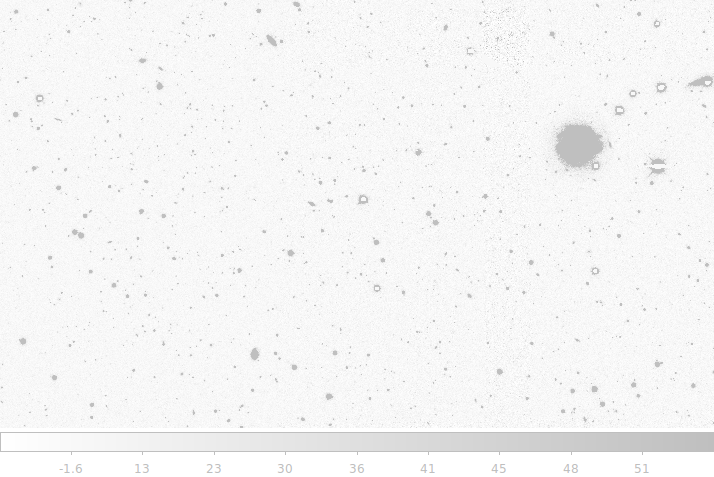
\includegraphics[height=23cm,angle=90,trim=4cm 2cm 0 0,clip]{./Pictures/ds9_transparent.png}}} % Image background

\end{document}
